\documentclass[12pt,a4paper]{article}
%packages
\usepackage[utf8]{inputenc}
\usepackage{amsmath}
\usepackage{amsfonts}
\usepackage{amssymb}
\usepackage{amsthm}
\usepackage{physics}
\usepackage{tikz-cd}
\usepackage{mathtools} % for text over and under iff etc, underset, underbrace etc

\usepackage{chngcntr}
\counterwithout{subsection}{section}
\setcounter{subsection}{-1}

\title{MT543 Topics in Algebra}
\author{Notes taken by Stephen Nulty and John Brennan}
\renewcommand{\abstractname}{Note:} 

%new commands
\newcommand{\nN}{\ensuremath{\mathbb{N}\,}}
\newcommand{\zZ}{\ensuremath{\mathbb{Z}\,}}
\newcommand{\rR}{\ensuremath{\mathbb{R}\,}}
\newcommand{\cC}{\ensuremath{\mathbb{C}\,}}
\newcommand{\hH}{\ensuremath{\mathbb{H}\,}}
\newcommand{\fF}{\ensuremath{\mathbb{F}\,}}
\newcommand{\qQ}{\ensuremath{a+bi+cj+dk\,}}
\newcommand{\nn}{\ensuremath{n \times n\,}}
\newcommand{\xonen}{\ensuremath{(x_1,x_2,\ldots, x_n)\,}}
\newcommand{\xonem}{\ensuremath{(x_1,x_2,\ldots, x_m)\,}}

\newcommand{\cinf}{\ensuremath{C^{\infty}\,}}
\newcommand{\cinfm}{\ensuremath{C^{\infty}(M)\,}}
\newcommand{\cinfn}[1]{\ensuremath{C^{\infty}(#1)\,}}
\newcommand{\tpm}{\ensuremath{T_p M}}
\newcommand{\teg}{\ensuremath{T_e G}} % tangent space of group at identity will probably be common
\newcommand{\tm}{\ensuremath{T M}}
\newcommand{\tn}[1]{\ensuremath{T {#1}}}
\newcommand{\tqn}[2]{\ensuremath{T_{#1} {#2}}}
\newcommand{\dfp}{\ensuremath{df_p \,}}
\newcommand{\dfq}[1]{\ensuremath{df_{#1}\,}}
\newcommand{\df}{\ensuremath{df}}
\newcommand{\dgq}[2]{\ensuremath{d {#1}_{#2}}}
\newcommand{\dg}[1]{\ensuremath{d {#1}}}

\newcommand{\mnr}{\ensuremath{M_n(\rR)\,}}
\newcommand{\mnc}{\ensuremath{M_n(\cC)\,}}
\newcommand{\mnh}{\ensuremath{M_n(\hH)\,}}
\newcommand{\mnf}{\ensuremath{M_n(\fF)\,}}
\newcommand{\mr}[1]{\ensuremath{M_{#1}(\rR)\,}}
\newcommand{\mc}[1]{\ensuremath{M_{#1}(\cC)\,}}
\newcommand{\mh}[1]{\ensuremath{M_{#1}(\hH)\,}}
\newcommand{\glnr}{\ensuremath{GL_n(\rR)\,}}
\newcommand{\glnc}{\ensuremath{GL_n(\cC)\,}}
\newcommand{\glnh}{\ensuremath{GL_n(\hH)\,}}
\newcommand{\glnff}{\ensuremath{GL_n(\fF)\,}}
\newcommand{\glnf}{\ensuremath{GL_n(\fF^n)\,}}
\newcommand{\glr}[1]{\ensuremath{GL_{#1}(\rR)\,}}
\newcommand{\glc}[1]{\ensuremath{GL_{#1}(\cC)\,}}
\newcommand{\glh}[1]{\ensuremath{GL_{#1}(\hH)\,}}

\newcommand{\gon}{\ensuremath{O(n)\,}}
\newcommand{\gun}{\ensuremath{U(n)\,}}
\newcommand{\gspn}{\ensuremath{Sp(n)\,}}
\newcommand{\gok}[1]{\ensuremath{O(#1)\,}}
\newcommand{\guk}[1]{\ensuremath{U(#1)\,}}
\newcommand{\gspk}[1]{\ensuremath{Sp(#1)\,}}

\newcommand{\gson}{\ensuremath{SO(n)\,}}
\newcommand{\gsun}{\ensuremath{SU(n)\,}}
\newcommand{\gsln}{\ensuremath{SL(n)\,}}
\newcommand{\gsok}[1]{\ensuremath{SO(#1)\,}}
\newcommand{\gsuk}[1]{\ensuremath{SU(#1)\,}}
\newcommand{\gslk}[1]{\ensuremath{SL(#1)\,}}
\newcommand{\zg}{\ensuremath{Z(G)\,}}
\newcommand{\zh}[1]{\ensuremath{Z\qty(#1)\,}}
\newcommand{\zlg}{\ensuremath{z(\lalg)\,}}
\newcommand{\zlh}[1]{\ensuremath{z\qty(\mathfrak{#1})\,}}

%lie algebras
\newcommand{\lglnr}{\ensuremath{\mathfrak{gl}_n(\rR)}}
\newcommand{\lglnf}{\ensuremath{\mathfrak{gl}_n(\fF)}}
\newcommand{\lgslnr}{\ensuremath{\mathfrak{sl}_n(\rR)}}
\newcommand{\lgslnf}{\ensuremath{\mathfrak{sl}_n(\fF)}}
\newcommand{\lgon}{\ensuremath{\mathfrak{o}_n}}
\newcommand{\lgson}{\ensuremath{\mathfrak{so}_n}}
\newcommand{\lgun}{\ensuremath{\mathfrak{u}_n}}
\newcommand{\lgsun}{\ensuremath{\mathfrak{su}_n}}
\newcommand{\lgspn}{\ensuremath{\mathfrak{sp}_n}}
\newcommand{\lalg}{\ensuremath{\mathfrak{g}}}
\newcommand{\lall}[1]{\ensuremath{\mathfrak{#1}}}

\newcommand{\sph}[1]{\ensuremath{S^{#1}}\,}
\newcommand{\tor}[1]{\ensuremath{T^{#1}}\,}
\newcommand{\rpk}[1]{\ensuremath{\mathbb{R}\mathrm{P}^{#1}}\,}

\newcommand{\ra}{\ensuremath{\Rightarrow}}
\newcommand{\la}{\ensuremath{\Leftarrow}}
\newcommand{\cin}{\ensuremath{\mathcal{I}_n\,}}
\newcommand{\ci}[1]{\ensuremath{\mathcal{I}_{#1}\,}}
\newcommand{\im}{\ensuremath{\operatorname{im}}}
\newcommand{\ol}[1]{\overline{#1}}
\newcommand{\ipm}[2]{\ensuremath{\left\langle #1, \, #2 \right\rangle}}
\newcommand{\ul}[1]{\underline{#1}}

\newcommand{\quot}[2]{\ensuremath{\;^{#1} / _{#2}\;}}
\newcommand{\ecomm}{\ensuremath{\comm{\cdot}{\cdot}}}
\newcommand{\commg}[2]{\ensuremath{\comm{#1}{#2}}_{\mathfrak{g}}}
\newcommand{\comml}[3]{\ensuremath{\comm{#1}{#2}}_{\mathfrak{#3}}}
\newcommand{\commp}[3]{\ensuremath{\comm{#1}{#2}}_{#3}}

\newcommand{\bij}[1]{\ensuremath{\operatorname{Bij}(#1)}}
\newcommand{\homeo}[1]{\ensuremath{\operatorname{Homeo}(#1)}}
\newcommand{\diffeo}[1]{\ensuremath{\operatorname{Diffeo}(#1)}}
\newcommand{\isom}[1]{\ensuremath{\operatorname{Isom}(#1)}}
\newcommand{\jac}[1]{\ensuremath{\operatorname{Jac}{#1}}}
\newcommand{\Ad}{\ensuremath{\operatorname{Ad}}}
\newcommand{\Adg}{\ensuremath{\operatorname{Ad}_g}}
\newcommand{\Adh}[1]{\ensuremath{\operatorname{Ad}_{#1}}}
\newcommand{\ad}{\ensuremath{\operatorname{ad}}}
\newcommand{\adx}{\ensuremath{\operatorname{ad}_X}}
\newcommand{\ady}[1]{\ensuremath{\operatorname{ad}_{#1}}}

\newcommand{\genericA}{\ensuremath{\pmqty{a_{11} & \ldots & a_{1n} \\ \vdots & \vdots & \vdots \\ a_{n1} & \ldots & a_{nn}}}}

% vertical and horizontal bars for matrix columns and rows.
\newcommand*{\vertbar}{\rule[-1ex]{0.5pt}{2.5ex}}
\newcommand*{\horzbar}{\rule[.5ex]{2.5ex}{0.5pt}}

%proofs etc
\newtheorem{thm}{Theorem}[subsubsection]
\newtheorem{defn}[thm]{Definition}
\newtheorem{lemma}[thm]{Lemma}
\newtheorem{prop}[thm]{Proposition}
\newtheorem{obs}[thm]{Observation}
\newtheorem{cor}[thm]{Corollary}

%block matrices
\newcommand{\rvline}{\hspace*{-\arraycolsep}\vline\hspace*{-\arraycolsep}}
\newcommand{\bigzero}{\mbox{\normalfont\Large\bfseries 0}}
\newcommand{\bigld}{\mbox{\normalfont\Large\bfseries \ldots}}
\newcommand{\bigvd}{\mbox{\normalfont\Large\bfseries \vdots}}

\renewcommand{\thesubsection}{§\arabic{subsection}}
\makeatletter
\def\@seccntformat#1{\@ifundefined{#1@cntformat}%
   {\csname the#1\endcsname\quad}%    default
   {\csname #1@cntformat\endcsname}}% enable individual control
\newcommand\section@cntformat{}     % section level 
\newcommand\subsection@cntformat{\thesubsection.\space} % subsection level
\newcommand\subsubsection@cntformat{\thesubsubsection.\space} % subsubsection level
\makeatother

\renewcommand{\thethm}{\arabic{subsection}.\arabic{subsubsection}.\arabic{thm}}

%begin
\begin{document}
\maketitle
\begin{abstract}
    Any transcription mistakes and typos are my own.
\end{abstract}
Lectures by David Wraith. Lie Groups and Lie Algebras.
\section{Lecture 1 25/09/23}
missed this lecture - some intro to do with spheres, transformations and symmetries and other motivational stuff. Definition of an algebra (bilinear product) over a field.

\subsection{Introduction}

Lie groups have a dual nature: they are groups but also very special topological spaces. The algebraic and topological (spatial) properties are closely aligned. Lie groups and Lie algebras lie at the intersection of algebra, topology, geometry, analysis and more.

\begin{defn}
An algebra is a vector space $V$ equipped with a bilinear map $m:V\times V \to V$.
\end{defn}

Note, the ``multiplication" map $m$ does not have to be commutative or associative. In general, Lie algebras are neither commutative nor associative. Recall,
\begin{align*}
&\mbox{Commutativity: } m(u, v) = m(v, u), \\
&\mbox{Associativity: } m(m(u, v), w) = m(u, m(v, w)).
\end{align*}
Every Lie group has an associated Lie algebra which encodes many properties of the group. Often this allows problems about Lie groups to be reduced to problems in (fancy!) linear algebra.

\subsection*{Example of a Lie group}

The set of rotations of a ball centred on $O$ in $\rR^3$ is a Lie group. It is a group under composition of rotations. To ``see" the topology here, notice that it makes sense to talk about two rotations being ``close", so there is a sense of space. It makes sense to consider a continuous family of rotations. Continuity implies the existence of topology. We can identify this group with the matrix group $SO(3)$. The map $\rR^3 \to \rR^3$ given by $x \mapsto Ax$ for $A \in SO(3)$ is a rotation and every rotation occurs in this way. $SO(3)$ is a subset (but not a subgroup) of the set/group of all $(3\times 3)$-real matrices $M_3(\rR)$. By listing the elements of any $3\times 3$ matrix we get a bijection $M_3(\rR) \to \rR^9$. As $\rR^9$ has a natural topology (metric), this gives a natural topology on $M_3(\rR)$ and by restriction on $SO(3)$.


\section{Lecture 2 27/09/23}
Sorting out tutorial times. Lectures: Monday 2pm MS2, Wednesday 2pm LGH, Thursday 12pm MS2.

Lie Groups, dual nature, Groups but also a topological geometrical character. Can prove things with a mix of both methods - intersection of various areas.

\subsection{Groups of matrices}
\subsubsection{General Linear Groups}

Quaternions will have a central role.

Consider groups of $N\times N$ matrices over the fields \rR and \cC and also over the quaternions.

\begin{defn}
The quaternions \hH is a 4-dim real vector space with standard basis elements $1,i,j,k$, equipped with an associative linear multiplication operation defined by

\[i^2=j^2=k^2=-1, \quad ij=k, jk=i, ki=j\]
\end{defn}

So a generic quaternion takes the form $a+bi+cj+dk$, $a,b,c,d \in \rR$.

Observe, $ji=j(jk)=(jj)k$ (by associativity) $=j^2k=-k$. Similarly $kj=-i$ and $ik=-j$.

e.g. $(2+i-3k)(5+2i-j+k)=10+4i-2j+2k+5i-2-k-j-15k-6j-61+3$ etc.

Quaternions is not commutative, so is not a field. However it is a skew field (division algebra).

Terminology - In $a+bi+cj+dk$, $a$ is called the real or scalar part, and the rest $bi+cj+dk$ imaginary or vector part.

In analogy with complex numbers,

\begin{defn} 
1. The conjugate of  \qQ , is $\overline{\qQ}=a-bi-cj-dk$
2. The norm of \qQ is  $|\qQ |=\sqrt{a^2+b^2+c^2+d^2}$
\end{defn}

Thus \hH is a normed vector space. Next observe that for each $q\in\hH$ $q\bar{q}=\bar{q}q = |q|^2$.

therefore (symbol) $q^{-1}=\bar{q}/|q|^2$. So $qq^{-1}=q\bar{q}/|q|^2=|q|^2=1$, similarly for $q^{-1}q=1$.

This allows division $q_1\cdot q_2^{-1}=q_1 \bar{q_2}/|q_2|^2$. Writing $q_1/q_2$ is ambiguous however. $q_1 q_2^{-1}\neq q_2^{-1} q_1$ generically.

Clearly $\rR \subset \cC \subset \hH$. A classic theorem of Frobenius asserts that \rR, \cC, \hH are the only real associative division algebras. These objects similarly play a distinguished role in Lie group theory.

Convention: Suppose V is a vector space over the quaternions \hH. We will adopt the convention that whenever we scale a vector $v\in V$ by a scalar $\lambda \in \hH$, we multiply on the left, i.e. $\lambda v$

Let $M_n(\rR),  M_n(\cC),  M_n(\hH)$ denote the sets (vector spaces!) of all $n\times n$ matrices over $\rR, \cC,  \hH$.

\begin{defn} 
The General Linear Groups $GL_n(\rR)$, resp. $GL_n(\cC)$ is the group of  $n\times n$ invertible matrices with \rR resp \cC coefficients. (Group under multiplication). Equivalently $GL_n(\rR)=\{A\in M_n(\rR)| \det(A)\neq0\}$. Similarly $GL_n(\cC)=\{A\in M_n(\cC)| \det(A)\neq0\}$.
\end{defn}

(return to the idea of determinants of quaternions later).

Recall that for any matrix $A\in\mnr$ we have two associated linear maps $L_A:\rR^n\to \rR^n, L_a(\vec{x})=A\vec{x},$  $R_A:\rR^n\to \rR^n, R_a(\vec{x})=\vec{x}A.$ 

It is well know that $A$ is invertible (RC cases) $\iff$ $\det(A)\neq0$ $\iff$ $L_A, R_A$ are isomorphisms.

\section{Lecture 3 02/10/23}
Thursday lecture moved to Friday at 10am in MS2.

Reminder: 
\begin{itemize}
\item Quaternions \hH, multiplication is associative not commutative. If $V$ is a \hH - vector space, we scale from the left only, i.e. $\lambda v$ for $\lambda \in \hH, v\in V$. 
\item General linear groups \glnr, \glnc groups under $*$ of all invertible \rR resp. \cC \nn - matrices.
\item $A\in \mnr, \mnc$ is invertible iff $\det A \neq 0$ iff $L_A, R_A$ are both invertible where $L_a(\vec{x})=A\vec{x}$, $R_a(\vec{x})=\vec{x}A.$ 
\end{itemize}

We now consider \mnh.

\begin{defn}
A function $f:\hH ^n \to \hH^n$ is \hH - linear if  $f ( \lambda _1 v_1+\lambda _2 v_2)=\lambda _1 f(v_1)+\lambda _2 f(v_2),\; \forall \lambda _1 \lambda _2 \in \hH , v_1,v_2 \in \hH ^n$.
\end{defn}

\begin{lemma}
For $A \in \mnh$, $R_A:\hH^n\to \hH^n$ given by $R_a(\vec{x})=\vec{x}A$  for $v\in \hH^n$ a row vector, is \hH - linear, however $L_A$ is in general not \hH - linear.
Proof: exercise
\end{lemma}

idea is that associativity makes $\lambda v A$ ok, but not with left multiplication which is interfered by commutativity.

\begin{lemma}
For $A \in \mnh$, $R_A:\hH^n\to \hH^n$, is an \hH - linear isomorphism iff $A$ is invertible, i.e. $\exists B\in \mnh$ such that $AB=BA=I_n$.
\end{lemma}

\begin{proof}
($\ra$) If $R_A$ is an iso. then there is a \hH -linear inverse $(R_A)^{-1}: \hH ^n \to \hH ^n $. There is a corresponding matrix $B\in \mnh$. Since $R_A \circ (R_A)^{-1}=R_A \circ (R_A)^{-1}=I_n$. we deduce $BA=AB=I_n$ (NB order of matrices here!). Therefore $B=A^{-1}$.

($\la$) Similar.
\end{proof}

\begin{defn}
The quaternionic general linear group $\glnh = \{A\in \mnh | A \text{ is invertible}\} = \{A\in \mnh| R_a \text{ is an iso.}\}$
\end{defn}

NB: There is a problem with the notion of \hH - determinant due to non-commutativity we'll return to this later (possible to define determinant and \glnh as ones with non-zero determinant, but defining it requires some thought.)

It turns out that we can view \cC and \hH- matrices/linear maps in terms of \rR- matrices. 

\begin{prop}
There is a real linear map $\rho_n: \mnc \to \mr{2n}$ such that the following diagram commutes. 
\begin{center}
\begin{tikzcd}
  \cC^n \arrow{d}{R_A} \arrow{r}{\theta_n}
    & \rR^{2n} \arrow{d}{R_{\rho_n(A)}} \\
  \cC^n \arrow{r}{\theta_n}
&\rR^{2n} \end{tikzcd}
\end{center}
where $\theta _n : \cC ^n \to \rR ^{2n}$ is given by $\theta _n (a_1+ib_1, \ldots , a_n+ib_n )=(a_1,b_1,\ldots, a_n,b_n)$.
\end{prop}

(compactly every complex matrix can be viewed as a real matrix of twice the size)

Remark: $\theta _n $ is  a real linear isomorphism. This forces $R_{\rho _n (A)}=\theta _n \circ R_A \circ \theta _n^{-1}$.

This is linear and therefore there is a corresponding matrix $\in \mr{2n}$.

\begin{proof}
Given that $\theta _n$ is a real-linear isomorphism, consider the map $\theta_n \circ R_A \circ \theta_n^{-1} : \rR^{2n} \to \rR^{2n}$. This is clearly real-linear, and hence corresponds to some $(2n\times 2n)$-real matrix which depends on $A$. Call this matrix $\rho_n(A)$. Thus we obtain a map $\rho_n (A) : \mnc \to \mr{2n}$, and the requirement that $\theta_n \circ R_A = R_{\rho_n (A)} \circ \theta_n$ is automatrically satisfied by construction. 

It remains to show that $\rho_n$ is a real-linear map. To this end we compute for $A_1, A_2 \in \mnc$ and $\lambda, \mu \in \rR$:

\begin{align*}
R_{\rho_n (\lambda A_1 + \mu A_2)} 
&= \theta_n \circ R_{\lambda A_1 + \mu A_2} \circ \theta_n^{-1} \\
&= \theta_n \circ (\lambda R_{A_1} + \mu R_{A_2}) \circ \theta_n^{-1} \\
&= \lambda \theta_n \circ R_{A_1} \circ \theta_n^{-1} + 
   \mu     \theta_n \circ R_{A_2} \circ \theta_n^{-1} \\
&= \lambda R_{\rho_n(A_1)} + \mu R_{\rho_n(A_2)} \\
&= R_{\lambda \rho_n(A_1) + \mu \rho_n(A_2)}.\\
\end{align*}
As for any $X, Y \in \mr{2n}$ we have $R_X = R_Y$ if and only if $X = Y$, we deduce that $\rho_n (\lambda A_1 + \mu A_2) = \lambda \rho_n(A_1) + \mu \rho_n(A_2)$ as required.
\end{proof}

\begin{obs}
$\rho_n$ is injective. Proof: exercise.
\end{obs}

\begin{lemma}
$\rho _n$ satisfies $\rho_n(AB)= \rho_n(A)\rho_n(B)$.
\end{lemma}

Remark: When we take 1.1.10 together with 1.1.9 and 1.1.8, we see that $\rho_n$ is an injective real-algebra homomorphism.

\begin{proof}
We compose commutative squares from 1.1.8 to get

\begin{center}
\begin{tikzcd}
  \cC^n \arrow{d}{R_A} \arrow{r}{\theta_n}
    & \rR^{2n} \arrow{d}{R_{\rho_n(A)}} \\
  \cC^n \arrow{r}{\theta_n}  \arrow{d}{R_B}
&\rR^{2n} \arrow{d}{R_{\rho_n(B)}} \\
  \cC^n \arrow{r}{\theta_n}
&\rR^{2n} 

\end{tikzcd}
\end{center}

On L.H.S. we have $R_B \circ R_A = R_{AB}$. (note order)

On R.H.S we have $R_{\rho_n(B)} \circ R_{\rho_n(A)} =R_{\rho_n(A)\rho_n(B)}$.

But since LHS is $R_{AB}$ this means $R_{\rho_n(AB)}= \text{composition on RHS}=R_{\rho_n(A)\rho_n(B)}$.
\end{proof}

It's not surjective however. Q: What exactly is $\rho_n(A)$? Consider $(a+ib)\in \mc{1}$. 

\[R_{(a+ib)}(x+iy)=(x+iy)(a+ib)=(ax-by)+i(ay+bx)\]

Now $\theta_1(x+iy)=(x,y) \in \rR^2$ etc.

So $\theta_1((ax-by)+i(ay+bx))=(ax-by,ay+bx)$

The corresponding map from $\rR ^2\to \rR^2$ is $(x,y)\mapsto (ax-by,ay+bx)$. Observe that 

\[\begin{pmatrix} x & y\end{pmatrix}\begin{pmatrix} a & b \\ -b & a \end{pmatrix}=(ax-by,ay+bx)\]

So $\begin{pmatrix} a & b \\ -b & a \end{pmatrix}\in \mr{2}$ corresponds under $\rho_1$ to $(a+ib)\in \mc{1}$.

More generally 

\[\begin{pmatrix}
  a_{11}+ib_{11} & \ldots &   a_{1n}+ib_{1n}\\
  \vdots & \vdots & \vdots \\
   a_{n1}+ib_{n1} & \ldots &   a_{nn}+ib_{nn}\\
\end{pmatrix} \in \mnc\]

corresponds to

\[
\begin{pmatrix}
  \begin{matrix}
  a_{11} & b_{11}  \\
  -b_{11} &   a_{11}
  \end{matrix}
  & \rvline & \bigld  & \rvline &
  \begin{matrix}
  a_{1n} & b_{1n}  \\
  -b_{1n} &   a_{1n}
  \end{matrix}  
  \\
\hline

  \bigvd
  & \rvline & \bigvd  & \rvline &
  \bigvd
  \\
\hline
    \begin{matrix}
  a_{n1} & b_{n1}  \\
  -b_{n1} &   a_{n1}
  \end{matrix}
  & \rvline & \bigld  & \rvline &
  \begin{matrix}
  a_{nn} & b_{nn}  \\
  -b_{nn} &   a_{nn}
  \end{matrix}  
\end{pmatrix} \in \mr{2n}
\]

 is obtained by replacing each \cC entry by its corresponding $2\times 2$ real block.

\section{Lecture 4 04/10/23}
Last time:

\begin{itemize}
\item $A\in \mnh$ then $R_A:\hH^n\to\hH^n$ given by $R_a(\vec{x})=\vec{x}A.$  is \hH - linear (assuming coefficients in \hH multiply on vectors from the left, x row vector). Left multiplication is not in general \hH linear.
\item Under the real linear isomorphism $\theta_n: \cC^n \to \rR^{2n},$ $\theta _n (a_1+ib_1, \ldots , a_n+ib_n )=(a_1,b_1,\ldots, a_n,b_n)$. Any complex-linear map $\cC^n\to \cC^n$ corresponds to a real-linear map $\rR^{2n}\to \rR^{2n}$ and in terms of matrices (an right multiplication) $A\in \mnc$ corresponds to some matrix $\rho_n(A)\in \mr{2n}$.
\item \[\text{If } A=\begin{pmatrix}
  a_{11}+ib_{11} & \ldots &   a_{1n}+ib_{1n}\\
  \vdots & \vdots & \vdots \\
   a_{n1}+ib_{n1} & \ldots &   a_{nn}+ib_{nn}\\
\end{pmatrix}\]
then 
\[
\rho_n(A)=\begin{pmatrix}
  \begin{matrix}
  a_{11} & b_{11}  \\
  -b_{11} &   a_{11}
  \end{matrix}
  & \rvline & \bigld  & \rvline &
  \begin{matrix}
  a_{1n} & b_{1n}  \\
  -b_{1n} &   a_{1n}
  \end{matrix}  
  \\
\hline

  \bigvd
  & \rvline & \bigvd  & \rvline &
  \bigvd
  \\
\hline
    \begin{matrix}
  a_{n1} & b_{n1}  \\
  -b_{n1} &   a_{n1}
  \end{matrix}
  & \rvline & \bigld  & \rvline &
  \begin{matrix}
  a_{nn} & b_{nn}  \\
  -b_{nn} &   a_{nn}
  \end{matrix}  
\end{pmatrix}
\]
\end{itemize}

Consider the \cC linear map $\cC^n\to \cC^n$ given by $z\to zi$. This is $R_A$ where 

\[A= \begin{pmatrix}
  i & \ldots &   0\\
  \vdots & \ddots & \vdots \\
   0 & \ldots &   i\\
\end{pmatrix} =iI\]

For this matrix we have 
\[\rho_n(A)=\begin{pmatrix}
  \begin{matrix}
  0 & 1  \\
  -1 &   0
  \end{matrix}
  & \rvline & \bigld  & \rvline &
  \bigzero
  \\
\hline

  \bigvd
  & \rvline & \bigvd  & \rvline &
  \bigvd
  \\
\hline
    \bigzero
  & \rvline & \bigld  & \rvline &
  \begin{matrix}
  0 & 1  \\
  -1 &   0
  \end{matrix}  
\end{pmatrix}=\cin
\]

A map $f:\cC^n\to \cC^n$ is \cC linear if it is real linear and $f(zi)=f(z)i$.

Let $bar{f}:\rR^{2n}\to \rR^{2n}$ be the corresponding \rR linear map and suppose this has matrix $B\in \mr{2n}$. Then the complex linearity requirement is $R_B\circ R_{\cin}=R_{\cin}R_{B}$. 

Since $R_X=R_Y \iff X=Y$ we see this is equivalent to asking $B\cin=\cin B$. i.e. $B\in \mr{2n}$ corresponds under $\theta_n$ to a complex linear map $\iff$  $B\cin=\cin B$.

We'd proved

\begin{cor}
The image of $\rho_n:\mnc \to \mr{2n}$ is the set of all of all matrices in \mr{2n} which commute with \cin .
\end{cor}

Remark: This shows that $\rho_n$ is not surjective.

\begin{lemma}
There is an injective group homomorphism $\rho_n : \glnc \to \glr{2n}$, given by restricting $\rho_n : \mnc \to \mr{2n}$.
\end{lemma}

\begin{proof}
We just have to check that if $A\in \glnc$, then $\rho_n(A)$ is invertible. Clearly $\rho_n(AA^{-1})=\rho_n(A^{-1}A)=\rho_n(I_n)$ so by 1.1.10. $\rho_n(A)\rho_n(A^{-1})=\rho_n(A^{-1})\rho_n(A)=\rho_n(I_n)=I_{2n}$. 

$\therefore \rho_n(A^{-1})=\rho_n(A)^{-1}$, hence $\rho_n(A)\in\glr{2n}$. So $\rho_n:\glnc\to\glr{2n}$, and by 1.1.10 this is a (multiplicative) group homomorphism 
\end{proof}

Now for quaternion matrices. 

First observe that there is a \cC linear isomorphism $\phi_n: \hH^n \to \cC^{2n}$ given by $\phi_n(z_1+w_1 j, \ldots, z_n+w_n j)=(z_1,w_1,\ldots,z_n, w_n).$

(exercise to figure out $a+bi+cj+dk$ as  $z+wj$, with $\rR\subset \cC \subset \hH$.)

\begin{prop}
There is an injective \cC linear map $\psi_n:\mnh \to \mc{2n}$ s.t. the following square commutes:

\begin{center}
\begin{tikzcd}
  \hH^n \arrow{d}{R_A} \arrow{r}{\phi_n}
    & \cC^{2n} \arrow{d}{R_{\psi_n(A)}} \\
  \hH^n \arrow{r}{\phi_n}
&\cC^{2n} \end{tikzcd}
\end{center}

i.e. $\phi_n\circ R_A = R_{\psi_n(A)}\circ \phi_n$. Moreover, $\psi_n$ satisfies $\psi_n(AB)=\psi_n(A)\psi_n(B)$.
\end{prop}

\begin{proof}
Analogous to that of prop 1.1.8 and lemma 1.1.10. Exercise! 
\end{proof}

Remark: It is easily checked (exercise!) that $\psi_1(z+wj) = \begin{pmatrix} z &w \\ -\bar{w}& \bar{z}\end{pmatrix}$

More generally, image of $\psi_n$ consists of block matrices with blocks of this form (analogous to $\rho_n$).

By restricting to invertible matrices we obtain:

\begin{cor}
There is an injective group homomorphism $\psi_n:\glnh \to \glc{2n}$.
\end{cor}
\begin{proof}
Analogous to 1.1.12 - exercise.
\end{proof}

( you can compose the maps then to get a real $4n$ matrix from a quaternionic one)

Composing $\rho_{2n}$ and $\psi_n$ gives

 \begin{cor}
There is an injective \rR linear map resp. group homomorphism given by $\rho_{2n}\circ \psi_n:\mnh \to \mr{4n}$ resp. $\rho_{2n}\circ \psi_n:\glnh \to \glr{4n}$.
\end{cor}

Slogan: all groups of \hH or \cC matrices can be viewed as groups of real matrices!

\begin{defn}
(1.1.16) For $A\in \mnh$, $\det(A):=\det \psi_n(A)$.
\end{defn}

\section{Lecture 5 06/10/23}

(Talking about matrices and linear maps, and in \rR , \cC and \hH, there's a standard basis given to go between linear maps and matrices.

\begin{center}
\begin{tikzcd}
  \cC^n \arrow{d} \arrow{r}
    & \cC^{n} \arrow{d} \\
  \rR^{2n} \arrow{r} 
&\rR^{2n} 
\end{tikzcd}
\end{center}
and you can go between \rR and \cC with a canonical map, where you forget the complex structure going to \rR from \cC or by pairing up the pairs of reals going to \cC .)

Last time:

\begin{itemize}
\item There is a canonical \cC linear isomorphism $\phi_n:\hH^n\to \cC^{2n}$ given by $\phi_n(z_1+w_1 j, \ldots, z_n+w_n j)=(z_1,w_1,\ldots,z_n, w_n).$
\item There is an injective homomorphism of complex algebras $\psi_n: \mnh \to \mc{2n}$ such that the following diagram commutes
\begin{center}
\begin{tikzcd}
  \hH^n \arrow{d}{R_A} \arrow{r}{\phi_n}
    & \cC^{2n} \arrow{d}{R_{\psi_n(A)}} \\
  \hH^n \arrow{r}{\phi_n}
&\cC^{2n} 
\end{tikzcd}
\end{center}
\item If $A\in \mnh$ then $\det(A):=\det \psi_n(A)$.
\end{itemize}

\begin{prop}
(1.1.17 - need to fix the numbering) For $A\in \mnh$, $A$ is invertible $\iff \det A \neq 0$, i.e. $\glnh=\{A\in \mnh | \det A \neq 0\}$.
\end{prop}

\begin{proof}
We claim that $A$ is invertible $\iff$ $\psi_n(A)$ is invertible.

(\ra) This is immediate from the multiplicative properties of $\psi_n$ in 1.1.13.

(\la) In 1.1.14 we noted that the restricted map $\psi_n:\glnh\to\glc{2n}$ is a group homomorphism. $\therefore$ if $\psi_n(A)\in\glc{2n}$ (i.e. is invertible) for $A\in \mnh$, then since $\im \psi_n$ is a subgroup of $\glc{2n}$, $\exists B\in \glnh$ s.t.  $\psi_n(B)=[\psi_n(A)]^{-1}$. (Want to show now that $B$ is the inverse of $A$.)

We have $\psi_n(AB)=\psi_n(A)\psi_n(B)=\psi_n(A)[\psi_n(A)]^{-1}=I_{2n}$. But $\psi_n$ is injective, so we must have $AB=I_n$. Similarly $BA=I$. $\therefore B=A^{-1}$ i.e. $A$ is invertible.

So the claim is true. 
\begin{gather*}
\therefore A \text{ is invertible } \underset{\text{claim}}{\iff} \psi_n \text{ is invertible } \\ 
\underset{\text{elementary linear algebra}}{\iff} \det \psi_n(A)\neq 0 \underset{\text{defn 1.1.16}}{\iff} \det A \neq 0 
\end{gather*}
\end{proof}

\subsubsection{Orthogonal Groups}

From now on we will only consider (skew) fields \rR, \cC, \hH (=\fF). 

Recall that an inner product on a vector space $V$ over \fF is a map $\ipm{\,\,}{}:V\times V \to\fF$ which is bilinear (i.e. linear in each entry) and is positive definite, i.e. $\ipm{v}{v} \geq 0\; \forall v\in V$. If $v\neq 0, \ipm{v}{v}>0$. e.g. dot product in $\rR^n$.

\begin{defn}
\phantom{x}\\
\begin{itemize}
\item[a] The \underline{standard inner product} in $\fF^n$ is given by $\ipm{(x_1,\ldots,x_n)}{(y_1,\ldots,y_n)}$ $= x_1\bar{y_1}+\ldots + x_n\bar{y_n}$, where $\bar{y_i}$ is the conjugate of $y_i$. (If $y_i\in\rR$ then $\bar{y_i}=y_i$). This is the dot product if $\fF=\rR$, and is called a \underline{Hermitian} inner product if $\fF=\cC$ or \hH.
\item[b] The standard basis for $\fF^n$ is $(1,0,\ldots,0)$, $(0,1,\ldots,0)$, $\ldots $, $(0,0,\ldots,1)$.
\end{itemize}
\end{defn}

Remarks: As $x\bar{x}=\abs{x}^2$ for all $x\in \fF^n$ we see that $\ipm{x}{x}\geq 0  \forall x \in \fF^n$ for the standard inner products.

For $\lambda \in \fF$,

\begin{itemize}
\item $\ipm{\lambda x}{ y}=\lambda \ipm{x}{y}$
\item $\ipm{ x}{ \lambda y}=\ipm{x}{y}\bar{\lambda}$ (NB for $q_1,q_2\in \hH$ $\ol{q_1q_2}=\bar{q_2}\bar{q_1}$.)
\item $\ol{\ipm{ x}{y}}=\ipm{ y}{x}$.
\end{itemize}

In the real case, vectors $x,y$ are orthogonal if $\ipm{ x}{y}=0$. A basis $\{v_1,\ldots,v_n\}$ for $\rR^n$ is orthonormal if $\abs{v_i}=1 \forall i$ and $\ipm{ v_i}{v_j}=0$ for $i\neq j$.

Exactly the same language is used if $\fF = \cC, \hH$.

\begin{lemma}
$\{v_1,\ldots,v_n\} \in \cC^n$ is a (Hermitian) orthonormal basis $\iff \{\theta_n(v_1), \theta_n(iv_1), \ldots , \theta_n(v_n), \theta_n(iv_n)\}$ is an orthonormal basis for $\rR^n$. 

($\theta_n:\cC^n \cong \rR^{2n}$).
\end{lemma}

\begin{proof}
An easy computation sows that 

\[\underbrace{\ipm{x}{y}_\cC}_{\text{Hermitian I.P. on } \cC^n} = \underbrace{\ipm{\theta_n(x)}{\theta_n(y)}_\rR}_{\text{dot product on } \rR^n}+i\ipm{\theta_n(x)}{\theta_n(iy)}_\rR\].

Thus $\ipm{x}{y}=0 \iff  \ipm{\theta_n(x)}{\theta_n(y)}_\rR $ and $\ipm{\theta_n(x)}{\theta_n(iy)}_\rR $. The result now follows easily. (Exercise: complete the argument)
\end{proof}

\section{Lecture 6 09/10/23}
$v\cdot v =\abs{v}^2$
%
$v\cdot w = \abs{v}\abs{w}\cos\theta$
%
Dot product tells you about lengths and angles.
%
Last time:

\begin{itemize}
\item standard inner product in $\rR^n, \cC^n, \hH^n$ is given by $\ipm{x}{y}=\sum\limits_{i=1}^n x_i\bar{y}_i$.
($\bar{y}_i=y_i$ if $y_i\in \rR$)
\item $\ipm{x}{y}_{\cC^n}= \ipm{\theta_n(x)}{\theta_n(y)}_{\rR^{2n}}+i\ipm{\theta_n(x)}{\theta_n(iy)}_{\rR^{2n}}$
\item (1.2.2) If $\{z_1,\ldots, z_n\}$ is an orthonormal basis for $\cC^n$, then 
\[\{\theta_n(z_1), \theta_n(iz_1), \ldots , \theta_n(z_n), \theta_n(iz_n)\}\]
is orthonormal for $\rR^n$
\end{itemize}

\begin{lemma}
$\{q_1, \ldots , q_n)\}$ is an orthonormal basis for $\hH^n \iff$
\begin{gather*}
\{\theta_{2n}\circ\phi_{n}(q_1), \theta_{2n}\circ\phi_{n}(iq_1), \theta_{2n}\circ\phi_{n}(jq_1), \theta_{2n}\circ\phi_{n}(k q_1), \ldots, 
\\ \theta_{2n}\circ\phi_{n}(q_n), \theta_{2n}\circ\phi_{n}(iq_n), \theta_{2n}\circ\phi_{n}(jq_n), \theta_{2n}\circ\phi_{n}(k q_n)\}
\end{gather*}
is orthonormal for $\rR^{4n}$.

($\phi_n: \hH^n \to \cC^{2n},$  $\theta_{2n}: \cC^{2n} \to \rR^{4n}$) 
\end{lemma}
\begin{proof}
This follows in the manner of 1.2.2 from the easily established formula

\begin{gather*}
\ipm{x}{y}_{\hH^n}= 
\ipm{\theta_{2n}\circ\phi_{n}(x)}{\theta_{2n}\circ\phi_{n}(y)}_{\rR^{4n}}
+i\ipm{\theta_{2n}\circ\phi_{n}(x)}{\theta_{2n}\circ\phi_{n}(iy)}_{\rR^{4n}}\\
+j\ipm{\theta_{2n}\circ\phi_{n}(x)}{\theta_{2n}\circ\phi_{n}(jy)}_{\rR^{4n}}
+k\ipm{\theta_{2n}\circ\phi_{n}(x)}{\theta_{2n}\circ\phi_{n}(ky)}_{\rR^{4n}}
\end{gather*}
\end{proof}

\begin{defn}
\begin{itemize}
\item[1)] The \ul{orthogonal group} $O(n)$ is 

\[O(n)=\{A\in \glnr | \ipm{xA}{yA}_{\rR^{n}}=\ipm{x}{y}_{\rR^{n}}, \forall x,y \in \rR^n\}\]

\item[2)] The \ul{unitary group} $U(n)$ is 

\[U(n)=\{A\in \glnc | \ipm{xA}{yA}_{\cC^{n}}=\ipm{x}{y}_{\cC^{n}}, \forall x,y \in \cC^n\}\]

\item[3)] The \ul{symplectic group} $Sp(n)$ is 

\[Sp(n)=\{A\in \glnh | \ipm{xA}{yA}_{\hH^{n}}=\ipm{x}{y}_{\hH^{n}}, \forall x,y \in \hH^n\}\]
\end{itemize}
\end{defn}

\ul{Exercise}: Show $\gon , \gun ,\gspn$ are groups under multiplication.

\ul{Remark}: We could also define 

\[O(n)=\{A\in \glnr | \ipm{Ax}{Ay}_{\rR^{n}}=\ipm{x}{y}_{\rR^{n}}, \forall x,y \in \rR^n\}\]
\[U(n)=\{A\in \glnc | \ipm{Ax}{Ay}_{\cC^{n}}=\ipm{x}{y}_{\cC^{n}}, \forall x,y \in \cC^n\}\]

Exercise: show this agrees with 1.2.4

\begin{lemma}
For $\fF=\rR, \cC,\hH$ and $A\in \glnf$. The following are equivalent (tfae),

\begin{itemize}
\item[a)] $A \in \gon, \gun, \gspn$ (as appropriate),
\item[b)] $R_A$ maps $\fF^n$- orthonormal bases to $\fF^n$-orthonormal bases,
\item[c)] The rows of $A$ from an orthonormal for $\fF^n$,
\item[d)] $AA^*=I_n$ where $A^*=\bar{A}^T$.
\end{itemize}
\end{lemma}

\begin{proof}
(a)$\ra$(b) This is clear since by definition, multiplication by $A$ preserves the inner product and in particular preserves orthogonality and lengths.

(b)$\ra$(c) The standard basis for $\fF^n$ is orthonormal with respect to the standard inner product $\ipm{\,\,}{}_{\fF^n}$. By part (b) $R_A$ maps this orthonormal basis to another orthonormal basis. But $R_A(e_i)=i^{\text{th}}$ row of $A$. Hence rows of $A$ form an o.n. basis. (o.n. stands for orthonormal).

(c)$\iff$(d) Observe that $(AA^*)_{ij}=\sum\limits_k a_{ik}a^*_{kj}=\sum\limits_k a_{ik}\bar{a}_{jk}$. The rows of $A$ being o.n. means 

\[\ipm{i^{\text{th}}\text{ row of } A }{j^{\text{th}}\text{ row of } A }=\delta_{ij}\]

($\delta_{ii}=1$, $\delta_{ij}=0$ if $i\neq j$)

i.e. $\sum\limits_k^n a_{ik}\bar{a}_{jk}=\delta_{ij}$ (maybe color this to show it matches previous?)

i.e. $(AA^*)_{ij}=\delta_{ij} \iff AA^*=I_n$

(c)$\ra$(a) The rows of $A$ are o.n., i.e. $\sum\limits_k^n a_{ik}\bar{a}_{jk}=\delta_{ij}$.

\begin{align*}
\ipm{xA}{yA}_{\fF^n}&=\ipm{\left(\sum_l x_l a_{l1},\ldots, \sum_l x_l a_{ln}\right) }{\left(\sum_m y_m a_{m1},\ldots,\sum_m y_m a_{mn}\right)}\\
&=\sum_{k,l,m} x_l a_{lk} \overline{y_m a_{mk}}\\
&=\sum_{k,l,m} x_l a_{lk} \overline{a_{mk}}\overline{y_m }\\
&=\sum_{l,m} x_l\delta_{lm}\overline{y_m }\\
&= \sum_l x_l \bar{y}_l\\
&= \ipm{x}{y}_{\fF^n}
\end{align*}

\end{proof}

\section{Lecture 7 11/10/23}

\ul{Previously}:

\[O(n)=\{A\in \mnr | \ipm{xA}{yA}_{\rR^{n}}=\ipm{x}{y}_{\rR^{n}}, \forall x,y \in \rR^n\}\]
\[U(n)=\{A\in \mnc | \ipm{xA}{yA}_{\cC^{n}}=\ipm{x}{y}_{\cC^{n}}, \forall x,y \in \cC^n\}\]
\[Sp(n)=\{A\in \mnh | \ipm{xA}{yA}_{\hH^{n}}=\ipm{x}{y}_{\hH^{n}}, \forall x,y \in \hH^n\}\]

Note: other people might use $Sp$ and symplectic group for something related but not exactly the same (something like $Sp(n,\fF)$).

1.2.5 For $A \in \glnf$ t.f.a.e.

\begin{itemize}
\item[a)] $A\in \gon, \gun, \gspn$
\item[b)] $R_A$ maps \fF orthonormal bases to \fF orthonormal bases.
\item[c)] Rows of $A$ are an o.n. basis for $\fF^n$.
\item[d)] $AA^*=I$ where $A^*=\bar{A}^T$.
\end{itemize}

\ul{Remark}: It follows from this that

\begin{align*}
A\in \gon \iff A^{-1}&=A^T\\
A\in \gun \iff A^{-1}&=\bar{A}^T\\
A\in \gspn \iff A^{-1}&=\bar{A}^T\\
\end{align*}

i.e. we could define $\gon =\{A\in \mnr | A^{-1}=A^T\}$. 

(This follows from 1.2.5 (d), provided we can also show $A^*A=I$. The latter follows from the fact that if $AB=1$, $(A,B\in \mnf)$ then \ra $BA=I$. Why is this?)

By definition a matrix $\in \gon$ if the corresponding linear map preserves the dot product, i.e. preserves lengths and angles. What about $\gun$ and $\gspn$?

\begin{prop}
\phantom{a}\\
\begin{itemize}
\item[1)] $\rho_n(\gun)=\gok{2n}\cap \rho_n(\glnc)$.
\item[2)] $\psi_n(\gspn)=\guk{2n}\cap \psi_n(\glnh)$.
\item[3)] $\rho_{2n}\circ \psi_n(\gspn)=\gok{4n}\cap \rho_{2n}\circ\psi_n(\glnh)$.
\end{itemize}
\end{prop}

\begin{proof}
See Moodle
\end{proof}

This says that the real matrices corresponding to matrices in $\gun$ and $\gspn$ are precisely the dot-product (i.e. length and angle) preserving transformation which have the form of the real version a complex/quaterionic matrix.

We now give an alternative description of \gon , \gun , \gspn .

\ul{Starting point}: In $\rR^n$, the norm and dot product determine each other via a ``polarization'' formula.

\[\ipm{x+y}{x+y}=\ipm{x}{x}+2\ipm{x}{y}+\ipm{y}{y}\]

i.e. $\norm{x+y}^2=\norm{x}^2+\norm{y}^2+2\ipm{x}{y}$.

$\therefore \ipm{x}{y}=\frac{1}{2}\left(\norm{x+y}^2 -\norm{x}^2-\norm{y}^2 \right) $.

This shows that we could define orthogonal transformation to be those preserving all norms.

For $\gun, \gspn$, we have the following fact:

\begin{lemma}
$\norm{x}_{\cC^n}=\ipm{x}{x}_{\cC^n}$ is equal to $\norm{\theta_n(x)}_{\rR^{2n}}$. Similarly $\norm{x}_{\hH^n}=\norm{\theta_{2n}\circ \phi_n(x)}_{\rR^{4n}}$.
\end{lemma}

\begin{proof}
Exercise. (Hint: $\ipm{x}{y}_{\cC^n}=\ipm{\theta_n(x)}{\theta_n(y)}_{\rR^{2n}}+i\ipm{\theta_n(x)}{\theta_n(iy)}_{\rR^{2n}}$ etc.)
\end{proof}

\begin{prop}
\phantom{a}\\
\begin{itemize}
\item[1)] $\gon=\{A\in\glnr | \norm{xA}_{\rR^{n}}=\norm{x}_{\rR^{n}}, \forall x\in\rR^n\}$.
\item[2)] $\gun=\{A\in\glnc | \norm{xA}_{\cC^{n}}=\norm{x}_{\cC^{n}}, \forall x\in\cC^n\}$.
\item[3)] $\gspn=\{A\in\glnh | \norm{xA}_{\hH^{n}}=\norm{x}_{\hH^{n}}, \forall x\in\hH^n\}$.
\end{itemize}
\end{prop}

\begin{proof}
(1) is established by the polarization formula.

(2) We need to show that $A\in \glnc$ preserves all norms then $A\in \gun$. (if it preserves inner products it automatically preserves norms). But if $\norm{xA}_{\cC^{n}}=\norm{x}_{\cC^{n}} \forall x\in \cC^n$ we have

\begin{align*}
&\norm{\theta_n(xA)}_{\rR^{2n}}=\norm{\theta_n(x)}_{\rR^{2n}}\\
&\implies \norm{\theta_n(x)\rho_n(A)}_{\rR^{2n}}=\norm{\theta_n(x)}_{\rR^{2n}}\\
\end{align*}

$\therefore \rho_n (A)\in \gok{2n}$ by (1). By 1.2.6(1), $\rho_n(\gun)=\gok{2n}\cap \rho_n(\glnc)$ and since $\rho_n$ is injective, we conclude that $A\in \gun$ as required. 

\end{proof}

\section{Lecture 8 13/10/23}

coming up: semi-direct products of groups, group actions (on sets), basic topology.

%$\rtimes$ and $\ltimes$ for semi direct product, and $\lhd$ for normal subgroup for some reason.

\begin{prop}
For $A\in \gon, \gun, \gspn$ we have $\abs{\det A}=1$.
\end{prop}

\begin{proof}
For $A\in \gon$, $AA^T=I$ by 1.2.5(d). So $\det(AA^T)=\det(A)\det(A^T)=\det(A)^2=\det I =1$.

For $A\in \gun$, $A\bar{A}^T=I$ by 1.2.5(d). So $\det(A\bar{A}^T)=\det(A)\det(\bar{A}^T)=\det(A)\det(\bar{A})$. But $\det(\bar{A})=\ol{\det(A)}$. To see this, note that $\det(A)$ is a sum of products of entries of $A$, and for complex conjugation, $\ol{a+b}=\bar{a}+\bar{b}$ and $\ol{ab}=\bar{a}\bar{b}$. So then  $\det(A\bar{A}^T)\det(A)\ol{\det(A)}=\abs{\det(A)}^2=\det I =1$. As $\abs{z}\geq 0$, we see $\abs{\det(A)}=1$ implies $\abs{\det(A)}=1$.

For $A\in \gspn$, $\det A:=\det_{\cC} \psi_n(A)$. By 1.2.6(2) we know that $\psi_{n}(A)\in \guk{2n}$. $\therefore \det \psi_n(A)\ol{\det \psi_n(A)}=\det (\psi_n(A)\ol{ \psi_n(A^T)})=\det I=1$. $\therefore \abs{\det(\psi_n(A))}^2=1$, so $\abs{\det(\psi_n(A))}=1$ and $\therefore \abs{\det(A)}=1$
\end{proof}

\ul{Remark} For $A\in \gon$, $\det A =\pm 1$. 

For $A\in \gun$, $\det A \in \{e^{i\theta}\mid \theta \in [0,2\pi]\}.$ (circle in complex plane).

For $A\in \gspn$, it turns out that $\det A=1$. This is not obvious!

\begin{defn}
``Special Groups".\\

\begin{itemize}
\item[1)] The special orthogonal group $\gson = \{A\in \gon\mid \det A=1\}$,
\item[2)] The special unitary group $\gsun = \{A\in \gun\mid \det A=1\}$,
\item[3)] The special linear group $\gson = \{A\in \mnr (\text{ or } \glnr)\mid \det A=1\}$
\end{itemize}
\end{defn}

\ul{Remark}
\begin{itemize}
\item[1.] \gsln could be also written $SL(n,\rR)$ or $SL_n(\rR)$. Also have complex version $SL(n,\cC)$ with the obvious definition.
\item[2.] The significance of $\gsln$ is that this is the group of corresponding linear maps are precisely the volume preserving linear transformations. This follows from:
\item[3.] FACT: $A\in \mnr$. Then the volume of the parallelepiped determined by the vectors $R_A(e_1),\ldots,R_A(e_n)$ is $\abs{\det A}$. Exercise: prove this fact! ($\mathrm{vol}=\abs{\det A}$.

(insert vector picture).
\item[4.] \gspn is already special!
\end{itemize}

\ul{Question} What is the relationship between \gson and \gon, \gsun and \gun ?

\begin{thm}
$\gun = \gsun \rtimes \guk{1}$.
\end{thm}

$\rtimes$ is a semidirect product. Quick definition: $G$ is a semidirect product of subgroups $N,H$ if 
\begin{itemize}
\item[1)] $N\lhd G$,
\item[2)] $G=NH$ i.e. $G=\{nh\mid n\in N, h\in H\}$,
\item[1)] $N\cap H =\{e\}$.
\end{itemize}

\ul{Remark} $\guk{1}=\{(e^{i\theta})\mid \theta \in [0,2\pi]\}$ which we identify with $\{e^{i\theta} \mid \theta \in [0,2\pi] \}$. For the purposes of the theorem, we will identify $\guk{1}$ with $\pmqty{\dmat{e^{i\theta},1,\ddots,1}}$.

\begin{proof}
We observe that $\gsun \lhd \gun$ since $\gsun$ is the kernel of $\det : \gun \to \{e^{i\theta} \mid \theta \in [0,2\pi] \}$. ($\det$ is a homomorphism and kernel of any homomorphism is normal.)

Next observe that any $A=\pmqty{a_{11} & \ldots & a_{1n} \\ \vdots & \vdots & \vdots \\ a_{n1} & \ldots & a_{nn}} \in \gun$ can be expressed as a product

\[A=\pmqty{ \frac{1}{\det A} a_{11} & a_{12} & \ldots & a_{1n} \\ \frac{1}{\det A} a_{21} & a_{22} & \ldots & a_{2n} \\ \vdots & \vdots & \ldots & \vdots \\ \frac{1}{\det A} a_{n1} & a_{n2} & \ldots & a_{nn}}\pmqty{\dmat{\det A, 1, \ddots, 1}}\]

As $A$ and $\pmqty{\dmat{\det A, 1, \ddots, 1}}$ are both $\in \gun$, so is left hand matrix above.

Moreover, $\det$ of L.H. matrix is $\frac{1}{\det A}$ is $\frac{1}{\det A}\det A = 1$. $\therefore $ L.H. matrix $\in \gsun$. It remains to show $\gsun \cap \guk{1}=\{e\}$.
\end{proof}

This is clear since any matrix of the form $\pmqty{\dmat{e^{i\theta},1,\ddots,1}}$ with $\det =1$ must be $I_n$. Analogous arguments show 

\begin{thm}
$\gon =\gson \rtimes \zZ_2$.
\end{thm}

\begin{proof}
exercise.
\end{proof}

\section{Bonus Lecture 1: Semidirect products of groups}

Direct product: $G,H$ can form $G\times H=\{(g,h)\mid g\in G, h\in H\}$ with multiplication given by $(g,h)\cdot (g',h')=(gg',hh')$. (External direct product).

Now suppose that $G$ has subgroups $H,K$ such that $G=HK$, i.e. $G=\{hk \mid h\in H, k\in K\}$. What about multiplication in $G$?

$(hk)(h'k')=$? In the nicest case we might have $kh'=h'k$, so $(hk)(h'k')=hh'kk' \in HK$. This will work precisely when $H$ and $K$ commute with each other. In that case $G$ is an (internal) direct product of $H$ and $K$.

\ul{Definition} If $H,K\subset G$, then G is a direct product of $H$ and $K$ if
\begin{itemize}
\item[1)] $G=HK$
\item[2)] $H\cap K =\{e\}$ ( this means any expression $g=hk$ is unique)
\item[3)] $H,K$ commute with each other, i.e. $hk=kh$, $\forall h\in H, k\in K$,

(3) is often replaced by
\item[3')] $H \lhd G$, $K\lhd G$. (not equivalent by itself with 1 and 2 it is)
\end{itemize}

\ul{Definition} $G$ is a semidirect product of $K\subset G$ and $N\lhd G$ if (1) and (2) hold.

What's going on?

(Aside) $N\lhd G$ means $N$ is "normal" in $G$ i.e. $N\subset G$ with the following property $gNg^{-1}\subset N \forall g\in G$.

$\therefore$ for any $n\in N$ and any $g\in G$, $gng^{-1}=n'$ for some $n'\in N$, i.e. $gn=n'g$ (*).

If $G=NH$ then consider the product 
\begin{align*}
& (n_1h_1)(n_2h_2)\\
=& n_1(h_1n_2)h_2 \quad \text{associativity}\\
\underset{(*)}{=}& n_1n_2' h_1 h_2 \quad \in NH.
\end{align*}

\ul{Remark}
\begin{itemize}
\item[(1)] As a \ul{set} $N\rtimes H$ is just $N\times H$. But as a group it is in general a "twisted" product.
\item[(2)] Example dihedral groups $D_n$, where $D_n$ is the group of symmetries of a regular $n$-gon. $\abs{D_n}=2n$. There are two types of symmetries here:
\begin{itemize}
\item[i)] rotations about centre: subgroup isomorphic to $\cong \zZ_n$
\item[ii)] flips : subgroup $\cong \zZ_2$.
\end{itemize}
$D_n\cong Z_n \rtimes Z_2$ not a product since rotations and flips do not commute.
\item[(3)] There are several different looking ways to define a semidirect product. (e.g. short exact sequences, group extensions)
\end{itemize}

\section{Bonus Lecture 1: Group Actions}
Let $X$ be a set, and let $\bij{X}$ be the set of bijections $X\to X$. This a group under composition.

\ul{Definition} An action of a group G on the set $X$ is a homomorphism $\alpha:G\to \bij{X}$.

If X has some extra structure e.g. $X$ is a topological space, then we often replace \bij{X} with a group of bijections which preserve the extra structure.

For a topological space $X$ we consider $\alpha:G\to \underbrace{\homeo{X}}_{\text{group of "homeomorphisms"}}$.

\ul{Examples} 
\begin{itemize}
\item[i)]\glnr acts on $\rR^n$ by right or left multiplication. $\underbrace{R}_{\text{right multiplication}}:\glnr \to \underbrace{\operatorname{Isom}(\rR^n)}_{\text{group of linear isomorphisms of } \rR^n}$
\item[ii)] $\underbrace{\zZ_2}_{=\{\pm 1\}}$ acts on $\rR$ by flips about $0$. (picture of real line arrows indicating flips)
\item[iii)] \gsok{2} acts on the circle $S^1$, $\alpha:\gsok{2}\to \homeo{S^1}$. If $S^1=\{\pmqty{x \\ y} \in \rR^2\mid x^2+y^2=1\}$ then action is by matrix multiplication
\[\underbrace{\pmqty{\cos \theta & \sin \theta \\ -\sin \theta & \cos \theta}}_{\text{generic element of }\gsok{2}}\pmqty{x \\ y} = \underbrace{\pmqty{\cdot \\ \cdot}}_{\text{again element of }S^1}\]
\item[iv)] $\guk{1}=\{e^{i\theta}\}=$(circle) acts on $2$-sphere $S^2$ by rotation (picture of sphere rotation through line connection poles say).
\end{itemize}

\section{Bonus Lecture 1: Topology}
Everything topological in module can be interpreted in terms of metric spaces (but doing so might be needlessly cumbersome).

Recall a metric space consists of a set $X$ and a "metric" $d:X\times X\to [0,\infty)$ such that
\begin{itemize}
\item $d(x,y)=d(y,x)$
\item $d(x,y)=0 \iff x=y$
\item $d(x,z)\leq d(x,y)+d(y,z)$ (triangle).
\end{itemize}
$d$ is a \ul{distance function}.

An open ball in $(X,d)$: $B(p,r)=\{x\in X\mid d(p,x)<r\}$, $p\in X$, $r>0$.

Unions of open balls are called open sets. Metric allows us to define continuity and convergence.

It turns out that these notions can be describe using only open sets, e.g. $f:(X,d)\to (Y,d')$ is continuous $\iff$ for every open set $U\subset Y$, preimage $f^{-1}(U)$ is open in $X$. (*)

Open sets satisfy the following properties.
\begin{enumerate}
\item $X,\emptyset$ are open
\item unions of open sets are open
\item intersections of finitely many open sets are open.
\end{enumerate}

\ul{Definition} A topological space $(X,T)$ is a set $X$ together with a collection of subsets $T$ ("topology") satisfying (1), (2), (3).

\ul{Remark} Every metric space is a topological space. Many different metrics on $X$ will generate the same topology (collection of open sets). Not every topology $T$ will arise from a metric (more general in a sense).

\ul{Definition} A homeomorphism $f:(X,T)\to (Y,T')$ such that
\begin{enumerate}
\item $f$ is a bijection \&
\item $f,f^{-1}$ are both continuous as in (*) 
\end{enumerate}

\ul{Other terms}
\begin{enumerate}
\item A subset $C$ of $(X,T)$ is \ul{closed} if $X\setminus C \in T$, i.e. $X\setminus C$ is open.
\item A subset $S\subset (X,T)$ is \ul{compact} if every collection of $S$ by open sets in $X$ has a finite subcovering (i.e. still covering $S$). \ul{idea} Compact is small and neat (highly non technical)
\item A topological space is path-connected if you can join any two points by a continuous path ($p:\underset{\text{standard metric topology}}{[0,1]}\to (X,T)$)
\item A space is simply connected if any continuous loop in space can be contracted through the space to a point. Write this as $\pi_1(\underset{X}{\text{space}})=0$.

For any space $\pi_1(X)$ is the "fundamental group" of  $X$ and measures the failure of loops to be contractible. (e.g. Circle has fundamental group isomorphic to \zZ).
\end{enumerate}

\section{Lecture 9 16/10/23}
\ul{Last time}
\begin{itemize}
\item $\gun \cong \gsun \rtimes \guk{1}$, here \guk{1} is identified with $\{\pmqty{\dmat{e^{i\theta},1,\vdots,1}}\}\cong \guk{1}$.
\item $\gon \cong \gson \rtimes \zZ_2$, where $\zZ_2 = \{I,\pmqty{\dmat{-1,1,\vdots,1}} \}$
\end{itemize}

\begin{defn}
Metric spaces $(X,d)$ and $(Y,d')$ are \ul{isometric} if $\exists$ bijection $f:X\to Y$ s.t. $d'(f(x_1),f(x_2))=d(x_1,x_2), \, x_1, x_2 \in X$. $f$ is an \ul{isometry}. (distance preserving maps) 
\end{defn}

In $\rR^n$ we have a standard distance $d_{st}$ and a norm related by $d_{st}=\norm{x_1-x_2}(=\ipm{x_1-x_2}{x_1-x_2}^{1/2})$.

By 1.2.8 ($\gon=\{A\in \mnr \mid \underset{=\norm{R_A(x)}}{\norm{xA}}=\norm{x}, \forall x \in \rR^n\}$), we see that if $A\in \gon$ then $R_A:\rR^n\to\rR^n$ is an isometry.

Sort of conversely:

\begin{prop}
Suppose $f:\rR^n\to \rR^n$ is an isometry (for $d_{st}$) which fixes $0\in \rR^n$, (i.e. $f(0)=0$) then $f=R_A$ for some $A\in \gon$. In particular $f$ is linear.
\end{prop}

\begin{proof}
see moodle. (reasonably straightforward but takes time to write out).
\end{proof}

\ul{Remark} The above establishes the fact that \gon is precisely the group of origin fixing isometries of $\rR^n$. (\gon is a group of matrices, but every matrix corresponds to a linear transformation in the standard basis)

What about isometries of $\rR^n$ that do not fix the origin?

Observe that for any $v\in \rR^n$, the translation map $T_v:\rR^n\to\rR^n$, $x\mapsto x+v$ is an isometry.

\begin{thm}
$\isom{\rR^n}$, the group of isometries of $\rR^n$ (under composition) is $\isom{\rR^n}\cong \rR^n \rtimes \gon$, where $\rR^n \cong \{T_v \mid v\in \rR^n\}$. In particular, any isometry is a composition of an orthogonal transformation and a translation.
\end{thm}

\begin{proof}
Exercise. (think about what happens to the origin - say to a point $v$, translate by $-v$ and then a origin fixing transformation is orthogonal.)
\end{proof}

\subsubsection{Basic topology of groups of matrices}
All groups of matrices seen so far are sub\ul{sets} of \mnf for $\fF=\rR,\cC,\hH$, and $\therefore$ bijective with subsets of $\mnr, \mr{2n}, \mr{4n}$ respectively.

Observe that there is a bijection $b:\mnr \to \rR^{n^2}$, given by 

\[b\left(\genericA \right)=(a_{11},a_{12},\ldots,a_{1n},a_{21},\ldots,a_{nn}).\]

The standard topology on $\rR^{n^2}$ can be "pulled-back" to give a natural topology on $\mnr$ which makes $b$ a homeomorphism (continuous bijection with continuous inverse). 

$\therefore$ all matrix groups seen so far inherit a (subspace) topology from some $\mnr \cong \rR^{n^2}$.

\begin{obs}
With respect to these natural topologies, the functions $\det$ and $\tr$ (trace) are continuous.
\end{obs}

\begin{defn}
\phantom{a}
\begin{itemize}
\item[1)] A \ul{matrix group} (as opposed to a group of matrices!) is a subgroup of $\glnff$ which is closed.
\item[2)] A \ul{topological group} is a group $G$ which is equipped with a topology with respect to which the operations of multiplication and inverse are continuous.
\end{itemize}
\end{defn}

\ul{Remark} The point of the closed condition in (1) is that it keeps the topology `nice'.

\begin{prop}
All groups seen so far are matrix groups
\end{prop}
\begin{proof}
View $\det$ as a map $\det:\glnr \to \rR$. This is continuous. $\gsln := \underset{\text{(pre-image)}}{\det ^{-1}\{1\}}$. As $\{1\}\subset \rR$ is closed, so is its pre-image $\therefore \gsln$ is a matrix group. Ditto $\gslk{n,\cC}$ etc.

($\rR \setminus \{1\}=(-\infty,1)\cup(1,\infty)$ is open).

For $\gon, \gun, \gspn$ consider the map $f:\glnff\to\glnff$ given by $f(A)=AA^*$. $f^{-1}(I)=\gon, \gun, \gspn$ depending on $\fF$. As $f$ is continuous and $\{I\}$ is closed in $\glnff$, we see $\gon, \gun, \gspn$ are closed in $\glnff$.

Finally $\gsun=\gun \cap \gslk{n,\cC}$. $\gson=\gon \cap \gsln$, and intersection of closed sets is closed. Hence these are matrix groups. 
\end{proof}

\section{Lecture 10 18/10/23}
\ul{Previously} 
\begin{itemize}
\item $\rR^n $ has a standard (metric) topology. 

Bijection $b:\mnr \to \rR^{n^2}$. 

"Pull-back" metric/topology to \mnr.

\mnf bijective to a subset of \mnr, \mr{2n}, \mr{4n} 

$\to$ \mnf has a natural topology. By restriction, so do all groups seen.

\item Matrix group $:=$ closed subgroup of \glnff
\end{itemize}

(Aside: compactness $[0,1]$ is compact, but $(0,1)$ isn't as $(0,1)\cong \rR$, $\sim$ compact is like small but has to make sense topologically, small caveat to intuitiveness)

\begin{prop}
\gon, \gson, \gun, \gsun, \gspn are compact
\end{prop}

\begin{proof}
We prove \gon is compact. Arguments for other groups analogous.

Consider a map $f:\mnr\to\mnr$ given by $f(A)=AA^T$. $\gon=f^{-1}(\{I\})$. As $\{I\}$ is a closed subset of \mnr and $f$ is continuous, we see \gon is a closed subset of \mnr.

We have a homeomorphism $b:\mnr \to \rR^{n^2}$. $\therefore b(\gon)$ is closed in $\rR^{n^2}$.

Recall the Heine-Borel Thm: a subset of Euclidean space is compact $\iff$ it is closed and bounded.

It remains to show that $b(\gon)$ is bounded. (so then $b(\gon)$ is compact in $\rR^{n^2}$, and since $b$ is a homeomorphism preserving topologies, so \gon is compact in \mnr.)

Recall 1.2.5 the rows of any $A\in \gon$ form an orthonormal set. So each row is a unit vector in $\rR^n$. 
\[\norm{b(A)}=(\underbrace{a_{11}^2+a_{12}^2+\ldots +a_{1n}^2}_{=1}+\underbrace{a_{21}^2+\ldots +a_{2n}^2}_{=1}+\ldots+\underbrace{a_{n1}^2+\ldots+a_{nn}^2}_{=1})^{1/2}\]

$\therefore \norm{b(A)}=\sqrt{n}$.

$\therefore b(\gon)\subset$ sphere in $\rR^{n^2}$ of radius $\sqrt{n}$.

$\therefore b(\gon)$ is bounded as required.

\end{proof}

\begin{prop}
\glnff, \gspk{n,\fF} are non-compact.
\end{prop}

\begin{proof}
exercise
\end{proof}

\underline{Low dimensional examples}

$\gok{1}=\{(1),(-1)\}\cong \zZ_2$, $\gsok{1}=\{(1)\}$ trivial.

$\gsok{2}=\{\pmqty{\cos\theta & \sin\theta \\ -\sin\theta & \cos\theta} \mid \theta \in [0,2\pi )\}\underset{\text{isomorphic \& homeomorphic}}{\cong} \{e^{i\theta}\mid \theta \in [0,2\pi )\}\underset{\text{homeo}}{\cong} S^1$.

$\guk{1}=\{(e^{i\theta})\mid \theta \in [0,2\pi )\}$, $\therefore \gsok{2}\underset{\text{ homeo \& isomorphic }}{\cong}\guk{1}$.

$\gsuk{1}$ is trivial.

$\gsuk{2}=\{\pmqty{z & w \\ -\bar{w} & \bar{z}} \mid z,w \in \cC, \, \abs{z}^2+\abs{w}^2=1\}$. Now $\{(z,w) \in \cC^2 \mid \abs{z}^2+\abs{w}^2=1\}\underset{\text{homeo}}{\cong}  \{(x_1,x_2,x_3,x_4) \in \rR^4 \mid \sum\limits_{i=1}^4\abs{x_i}^2=1\}=S^3$, 3-sphere $\subset \rR^4$.

$\therefore$ as a topological space $\gsuk{2}\cong S^3$.

$\gspk{1}=\{(q)\mid q\bar{q}=1\}$, group of unit length quaternions.

As $\hH\cong \cC^2\cong \rR^4$ topologically/as real vector spaces, we see that $\gspk{1}\cong S^3$.

In fact \gspk{1} and \gsuk{2} are isomorphic as groups, with isomorphism given by $\psi_1$.

\ul{Observe} that all the above groups except \gok{1} are path-connected.

Recall that an action of a group $G$ on a set $X$ is a map $\alpha:X\times G\to X$ (this is a right action!) such that $\alpha(x,1)=x, \forall x\in X$ and $\alpha(\alpha(x,g),h)=\alpha(x,gh)$. 

For fixed $g\in G$ we obtain a map $\alpha_g :X\to X$ given by $\alpha(\cdot,g)$. This is a bijection with inverse $\alpha_{g^{-1}}$. 

$\therefore$ an action can be viewed as a homomorphism $\alpha: G\to \bij{X}$.  

e.g. a group can act on itself from left or right. i.e. $R_g:G\to G$, $R_g(g')=g'g$ etc.

If $X$ is a topological space then we replace $\bij{X}$ by $\homeo{X}$, so actions respect topology. 

Moreover, if $G$ has a topology we will assume action depends continuously on $g\in G$.

An action of $G$ on $X$ is transitive if for any points $x,y\in X$ $\exists g\in G$ s.t. $\alpha_g(x)=y$.

\begin{thm}
\label{transitive_action_on_sphere}
\hfill
\begin{enumerate}
\item \gson acts transitively by right (or left) multiplication on $\sph{n-1}\subset \rR^n$. \item Given any point $x\in \sph{n-1}$ there is a continuous path $p:[0,1]\to\gson$ s.t. $p(0)=I_n$ and $R_{p(1)}(e_1)=x$ ($n\geq 2$).
\end{enumerate}
\end{thm}

\ul{Remarks} $\gson$ acts by right/left mult. on $\rR^n$. As this action preserves distances it restricts to given an action on any sphere (say unit radius sphere) about $0$, $\sph{n-1}$, i.e. $R:\sph{n-1}\times \gson \to \sph{n-1}$.

\section{Lecture 11 20/10/23}

\begin{proof}
The first statement follows from the second (by composing paths as in Fig \ref{compose_paths}).

\begin{figure}
\center
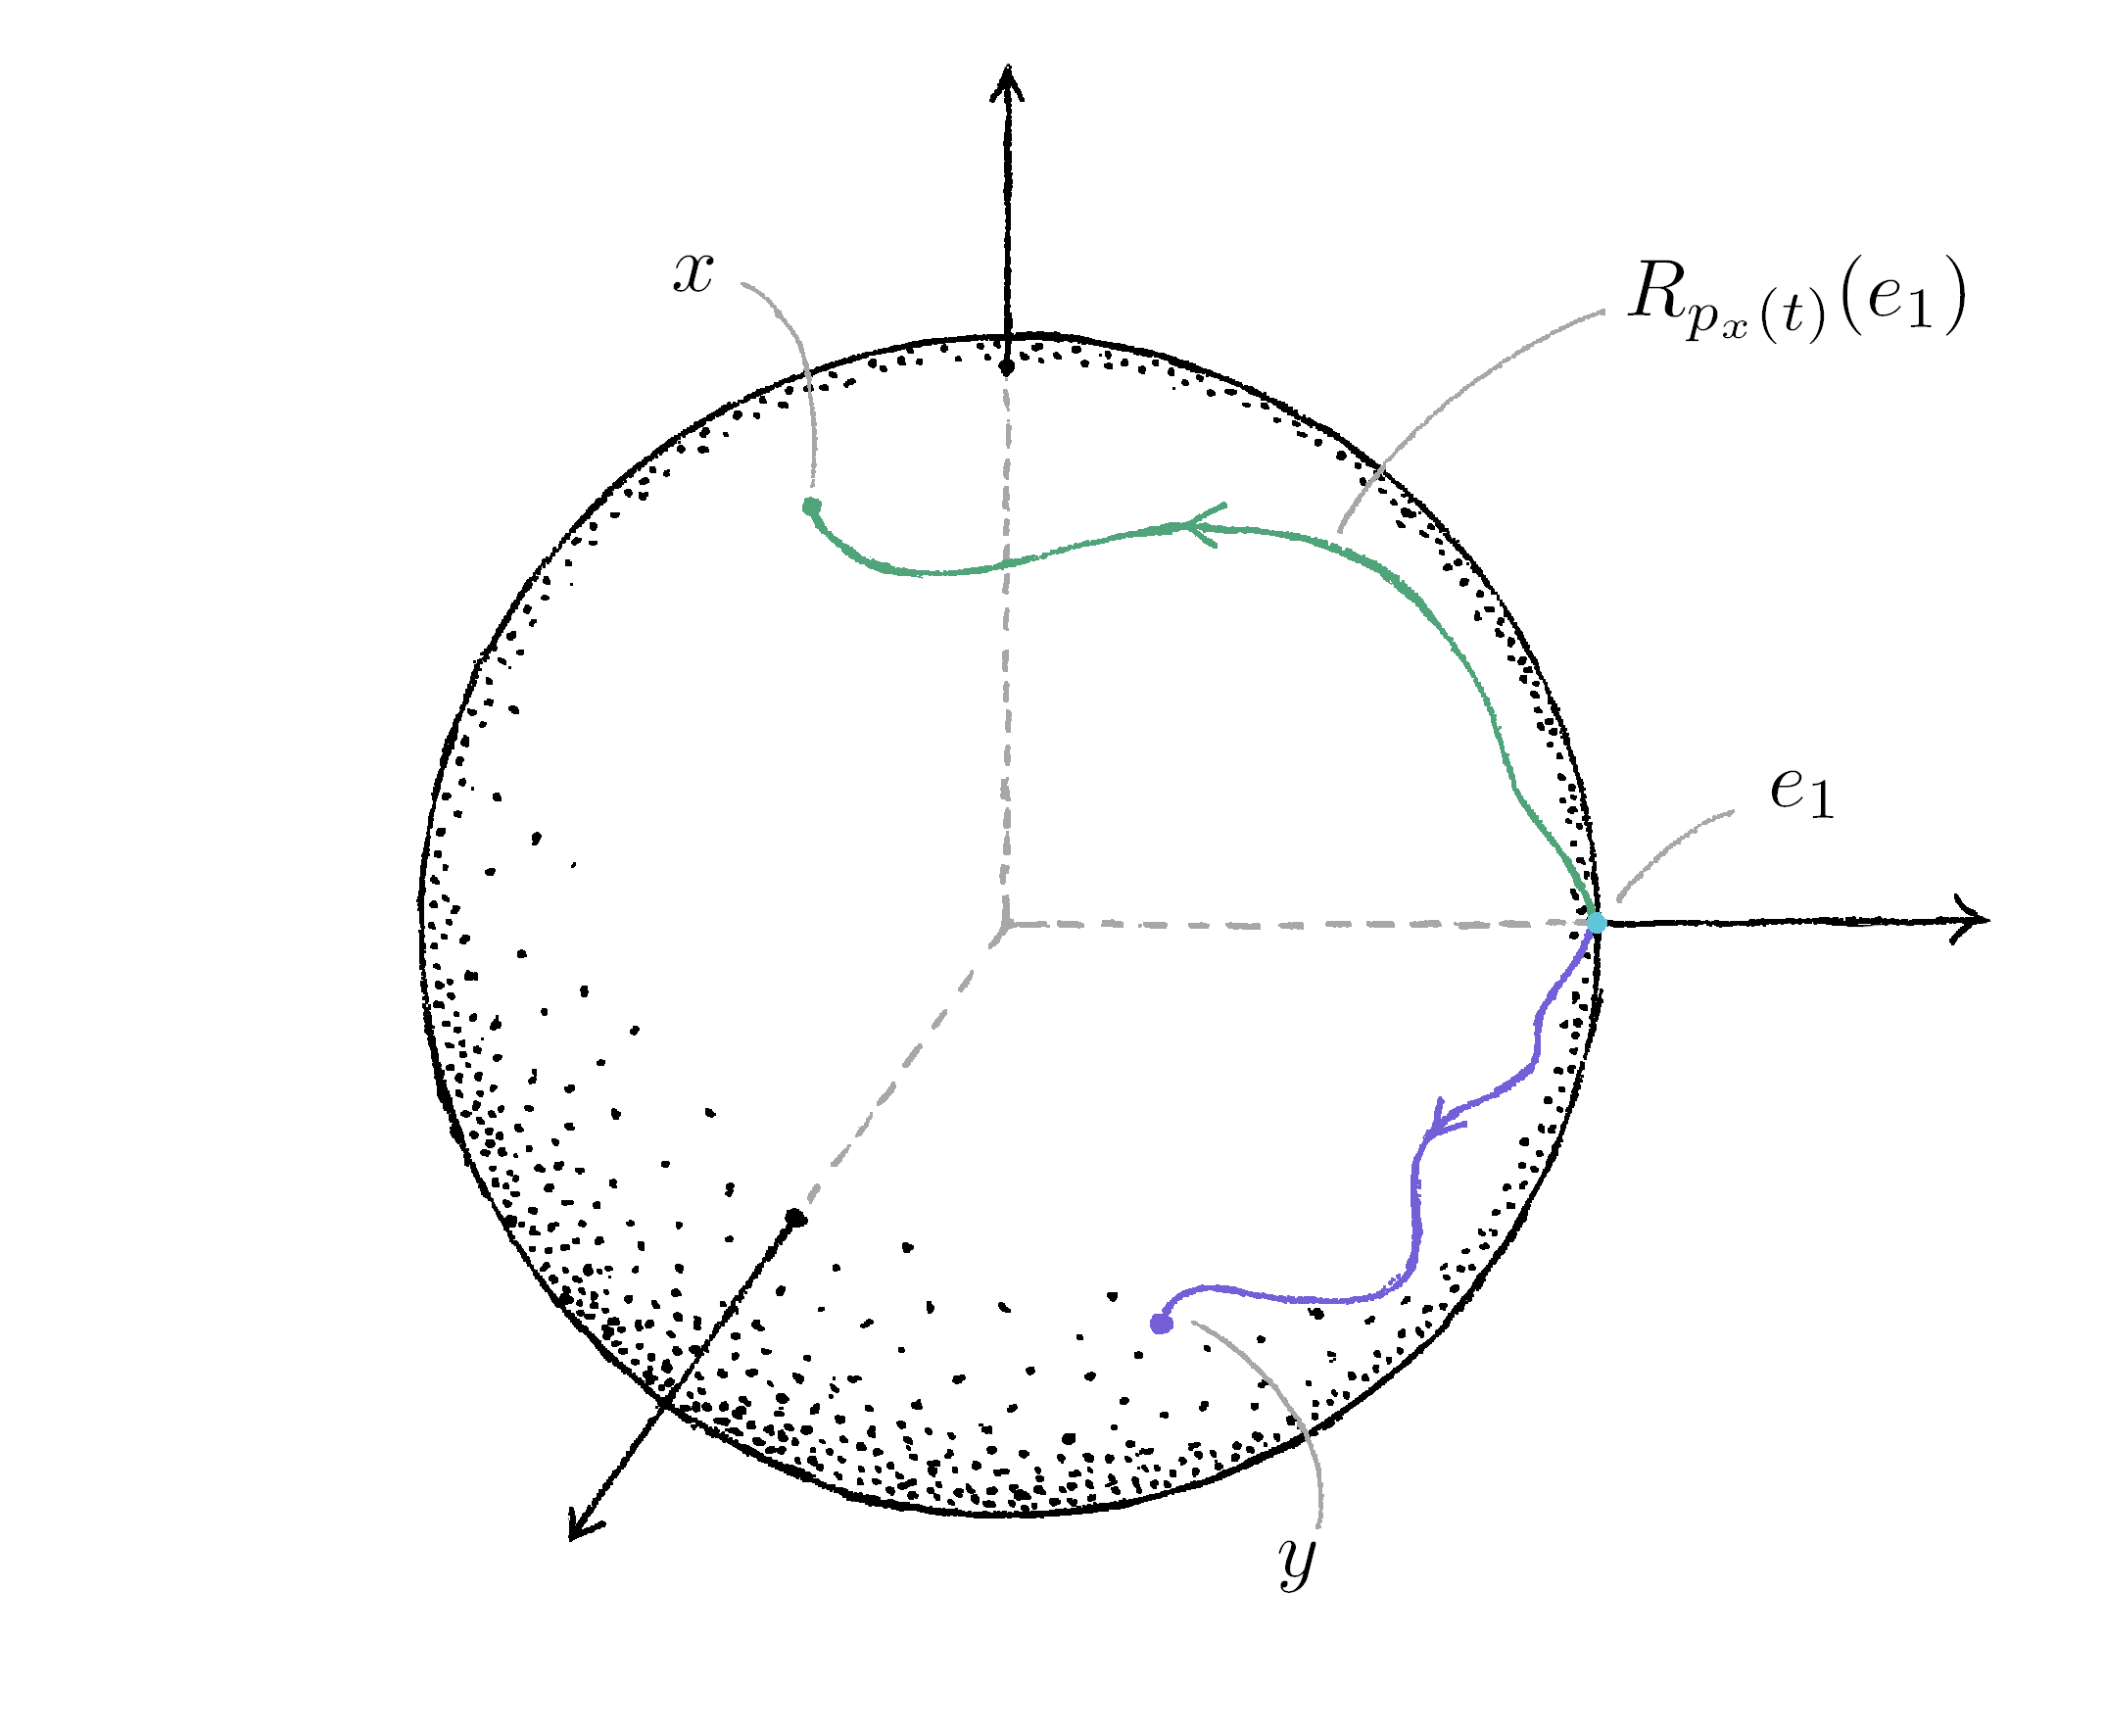
\includegraphics[scale=0.45]{figs/composing_paths/sphere_colour.png}
\caption{Here we depict the trajectories of $e_1$ in \sph{2} as it is evolved under paths in \gsok{3}, as decribed in \ref{transitive_action_on_sphere}, corresponding to points $x, y \in S^2$. Clearly, we can map $x$ to $y$ via $R_{p_x(1)}^{-1}\circ R_{p_y(1)}$.}
\label{compose_paths}
\end{figure}


For the second statement we proceed by induction. For $n = 2$ this is easy since
\[
\gsok{2} = \{\pmqty{\cos \theta & \sin \theta \\ -\sin \theta & \cos \theta}\mid \theta \in [0, 2\pi )\}.
\]
Clearly, for $x = (\cos\theta, \sin\theta) \in S^1$ we have a path
\[
p(t) = \pmqty{\cos (t\theta) & \sin (t\theta) \\ -\sin (t\theta) & \cos (t\theta)},
\]
such that $(1\ 0)p(t) = (\cos(t\theta)\ \sin(t\theta)$ which starts at $(1\ 0)$ and ends at $x$.
(insert figure of circle here)

Now assume the result is true for $n=k$ and consider \gsok{k+1} acting on $\rR^{k+1}$. We can write any $x \in S^k \subset \rR^{k+1}$ as $x = \cos\theta e_1 + \sin\theta y$ where $y \in \mbox{Span}\{e_2, \hdots, e_{k+1}\}$ is a unit vector. Choose a path $p_1(t)$ in \gsok{n} taking the form

\[
\begin{pmatrix}
  \begin{matrix}
  \cos(t\theta) & \sin(t\theta)  \\
  -\sin(t\theta) &   \cos(t\theta)
  \end{matrix}
  & \rvline & \bigzero
  \\
\hline

  \bigzero & \rvline &
  \ci{k-1}
\end{pmatrix}
\]
Observe that $R_{p_1(1)}(e_1) = \cos\theta e_1 + \sin\theta e_2$. Now, identify $\rR^k$ with $\mbox{Span}\{e_2, \hdots, e_{k+1}\}$. We know there exists a path $\bar{p}_2 : [0, 1] \to \gsok{k}$ such that $\bar{p}_2(0) = \mathcal{I}_k$ and $R_{\bar{p}_2(1)}(e_2) = y$ by the inductive hypothesis. By linearity $R_{\bar{p}_2(1)}(\sin(\theta) y) = \sin(\theta) y$. Now, we can define $p_2:[0, 1] \to \gsok{k+1}$ by
\[
p_2(t) =
\begin{pmatrix}
  1 & \rvline & 0
  \\
\hline

  0 & \rvline & \bar{p}_2(t)
\end{pmatrix}.
\]
Finally, define $p:[0, 1] \to \gsok{k+1}$ by
\[
p(t) =
\begin{cases}
p_1(2t)   & t \in  [0, \frac{1}{2}) \\
p_2(2t-1) & t \in  [\frac{1}{2}, 1].
\end{cases}
\]
By construction, $p(0) = \ci{k+1}$ and $R_{p(1)}(e_1) = \cos(\theta)e_1 + \sin(\theta)y = x$.
\end{proof}

\ul{Remark} Similar arguments apply to \gsuk{n} and \gspk{n} with very little change.

\begin{cor}
\gsok{n} is path-connected.
\end{cor}

\begin{proof}
For any $A \in \gsok{n}$ we construct a path from $A$ to \cin. By Lemma 1.2.5 the rows of $A$ form an orthonormal basis for $\rR^n$. Call these $r_1, \hdots , r_n$. By theorem 1.3.6 there exisits a path $p$ in \gsok{n} starting with \cin and ending with $p(1)$ which satisfies $R_{p_1(1)}(r_1) = e_1$. As matrices in \gsok{n} preserve orthonormality (by lemma 1.2.5) we see that $R_{p_1(1)}(r_i) \in \mbox{Span}\{e_2, \hdots , e_n\}$ for $i \geq 2$

Now let $s_2 = R_{p_1(1)}(r_2)$. By theorem 1.3.6, there exists a path $\bar{p}_2$ in \gsok{n-1} such that the corresponding path,
\[
p_2(t) =
\begin{pmatrix}
  1 & \rvline & 0
  \\
\hline

  0 & \rvline & \bar{p}_2(t)
\end{pmatrix},
\]
moves $s_2$ to $e_2$, ie $R_{p_2(1)}(s_2) = e_2$ (and $p_2(0) = \cin$). We can continue in this way to construct paths $p_i$ moving $r_i$ to $e_i$ but fixing $e_1, \hdots , e_{i-1}$. We can also compose these paths to obtain a path $p(t)$ such that $p(0) = \cin$ and $R_{p(1)}(r_i) = e_i$ for all $i$.

Finally, consider the $n\times n$ matrix obtained by stacking the images of $r_1, \hdots , r_n$ under $R_{p(t)}$:
\[
\begin{pmatrix}
  \horzbar & R_{p(t)}(r_1) & \horzbar \\
  \horzbar & R_{p(t)}(r_2) & \horzbar \\
  & \vdots &        \\
  \horzbar & R_{p(t)}(r_n) & \horzbar
\end{pmatrix}
\]
Notice that, for eact $t$, the rows are orthonormal, so this matrix is an element of \gsok{n} for all $t \in [0, 1]$. Moreover, at $t=0$ this matrix is
\[
\begin{pmatrix}
  \horzbar & r_1 & \horzbar \\
  \horzbar & r_2 & \horzbar \\
  & \vdots &        \\
  \horzbar & r_n & \horzbar
\end{pmatrix}
= A
\]
and at $t=1$
\[
\begin{pmatrix}
  \horzbar & e_1 & \horzbar \\
  \horzbar & e_2 & \horzbar \\
  & \vdots & \\
  \horzbar & e_n & \horzbar \\
\end{pmatrix}
= \cin
\]
Hence, we have constructe a path in \gsok{n} from $A$ to \cin.
\end{proof}

\section{Lecture 12 23/10/23}

Previously: 
\begin{itemize}
\item 1.3.6 \gson acts transitively on \sph{n-1}
\item 1.3.7 \gson is path-connected. 
\end{itemize}

\ul{Remark} Essentially the same arguments used in 1.3.6 \& 1.3.7 show

\begin{itemize}
\item \gsun, \gspn act transitively on \sph{2n-1} and \sph{4n-1} respectively.
\item \gsun , \gspn are path-connected. \gsln is also path connected, but the argument is different.
\end{itemize}

\begin{cor}
\gun is path connected by \gon has two path components (i.e. \ul{not} path connected).
\end{cor}

\begin{proof}
By 1.2.11, $\gun=\gsun \rtimes \guk{1}$. Topologically, $\gun \cong \gsun \times \sph{1}$ (forgetting the group structure), and is $\therefore$ path connected as \gsun and \sph{1} both are.

By 1.2.12, $\gon=\gson \rtimes \zZ_2$. Topologically this means $\gon \cong \gson \underset{\text{disjoint union}}{\amalg} \gson$. Hence $\gon$ has two path components, each $\cong \gson$. 
\end{proof}

\ul{Remark} $\zZ_2$ here corresponds to $\{I_n, \pmqty{\dmat{-1,1,\ddots,1}}\}$. The matrix $\pmqty{\dmat{-1,1,\ddots,1}}$ corresponds to a reflection in the hyperplane $\operatorname{span}\{e_2,\ldots,e_n\}$ (flipping the $e_1$ coordinate over). Notice that we can't have a continuous path from $I_n$ to $\pmqty{\dmat{-1,1,\ddots,1}}$ in $\gon$ as the determinant (which is continuous) would have to jump from $1$ to $-1$.

If we define a rotation of $\rR^n$ to be an origin fixing distance preserving map which can be linked via a continuous path of such maps to $I_n$, then we can deduce
\begin{itemize}
\item \gson is precisely the group of rotations of $\rR^n$,
\item \gon is precisely the group of rotations and reflections of $\rR^n$.
\end{itemize}

\ul{Final remark}:``Homogeneous spaces''.

If $G$ is a topological group and $H\subset G$ a subgroup, then the set of cosets $\quot{G}{H}$ ( or $_{H}\backslash ^{G}$) is a topological space with the quotient topology. $\quot{G}{H}$ is called a ``Homogeneous space'', as, when equipped with an appropriate geometry \quot{G}{H} ``looks'' the same at all points.

\ul{Examples} $\sph{n-1}\cong \quot{\gson}{\gsok{n-1}}\cong \quot{\gon}{\gok{n-1}}$, where \gsok{n-1} is identified with $\pmqty{\dmat{1,\gsok{n-1}}}\subset\gson$ etc.

$\sph{2n-1}\cong \quot{\gsun}{\gsuk{n-1}}\cong \quot{\gun}{\guk{n-1}}$

$\sph{4n-1}\cong \quot{\gspn}{\gspk{n-1}}$.

\subsection{Lie groups \& Lie Algebras}

\subsubsection{Manifolds}

Roughly speaking a manifold is a ``nice'' topological space such that a neighbourhood of each point ``looks like'' euclidean space of a fixed dimension. We can use the local euclidean property to transfer calculus (differential and with a bit more work integral) from $\rR^n$ to manifolds.

\begin{defn}
A topological $n$-manifold $M$ is a Hausdoff topological space with a countable basis for its topology, satisfying the following locally euclidean property: For any $x\in M$ there is an open set $x\in U\subset M$, and an open set $V\subset \rR^n$, and a homeomorphism $\phi:U \to V$.

(nice picture of torus, open sets, and arrow between it and $V$ in $\rR^n$).
\end{defn}

\ul{Remarks}
\begin{itemize}
\item[1)] $n$ is the ``dimension'' of the manifold.
\item[2)] The map $\phi$ is called a ``chart''.
\item[3)] A locally Euclidean space  which is a subset of some $\rR^m$ $m\geq n$ is automatically Hausdorff and has a countable basis for its topology.
\end{itemize}

\section{Lecture 13 25/10/23}

\ul{Previously} 2.1.1 A topological $n$-manifold $M$ is a Hausdoff topological space with a countable basis for its topology,which is locally euclidean, i.e. for each $x\in M  \exists U\subset M$ open with $x\in U$ and a homeomorphism $\phi:U \to V$, where $V\subset \rR^n$ is an open set. $\phi$ is a ``chart''. 

\begin{defn}
A family of charts $\{\phi_\alpha \mid \alpha \in \Lambda \}$ ($\Lambda$ an indexing set) on a manifold $M$ is called an \ul{atlas} if for each $x\in M$ $\exists \alpha \in \Lambda$ s.t. $x\in $ domain of $\phi_\alpha$.
\end{defn}

\ul{Remark} The inverse of any chart provides $M$ with a local coordinate system. See figure \ref{coord_patch}.

\begin{figure}
\center
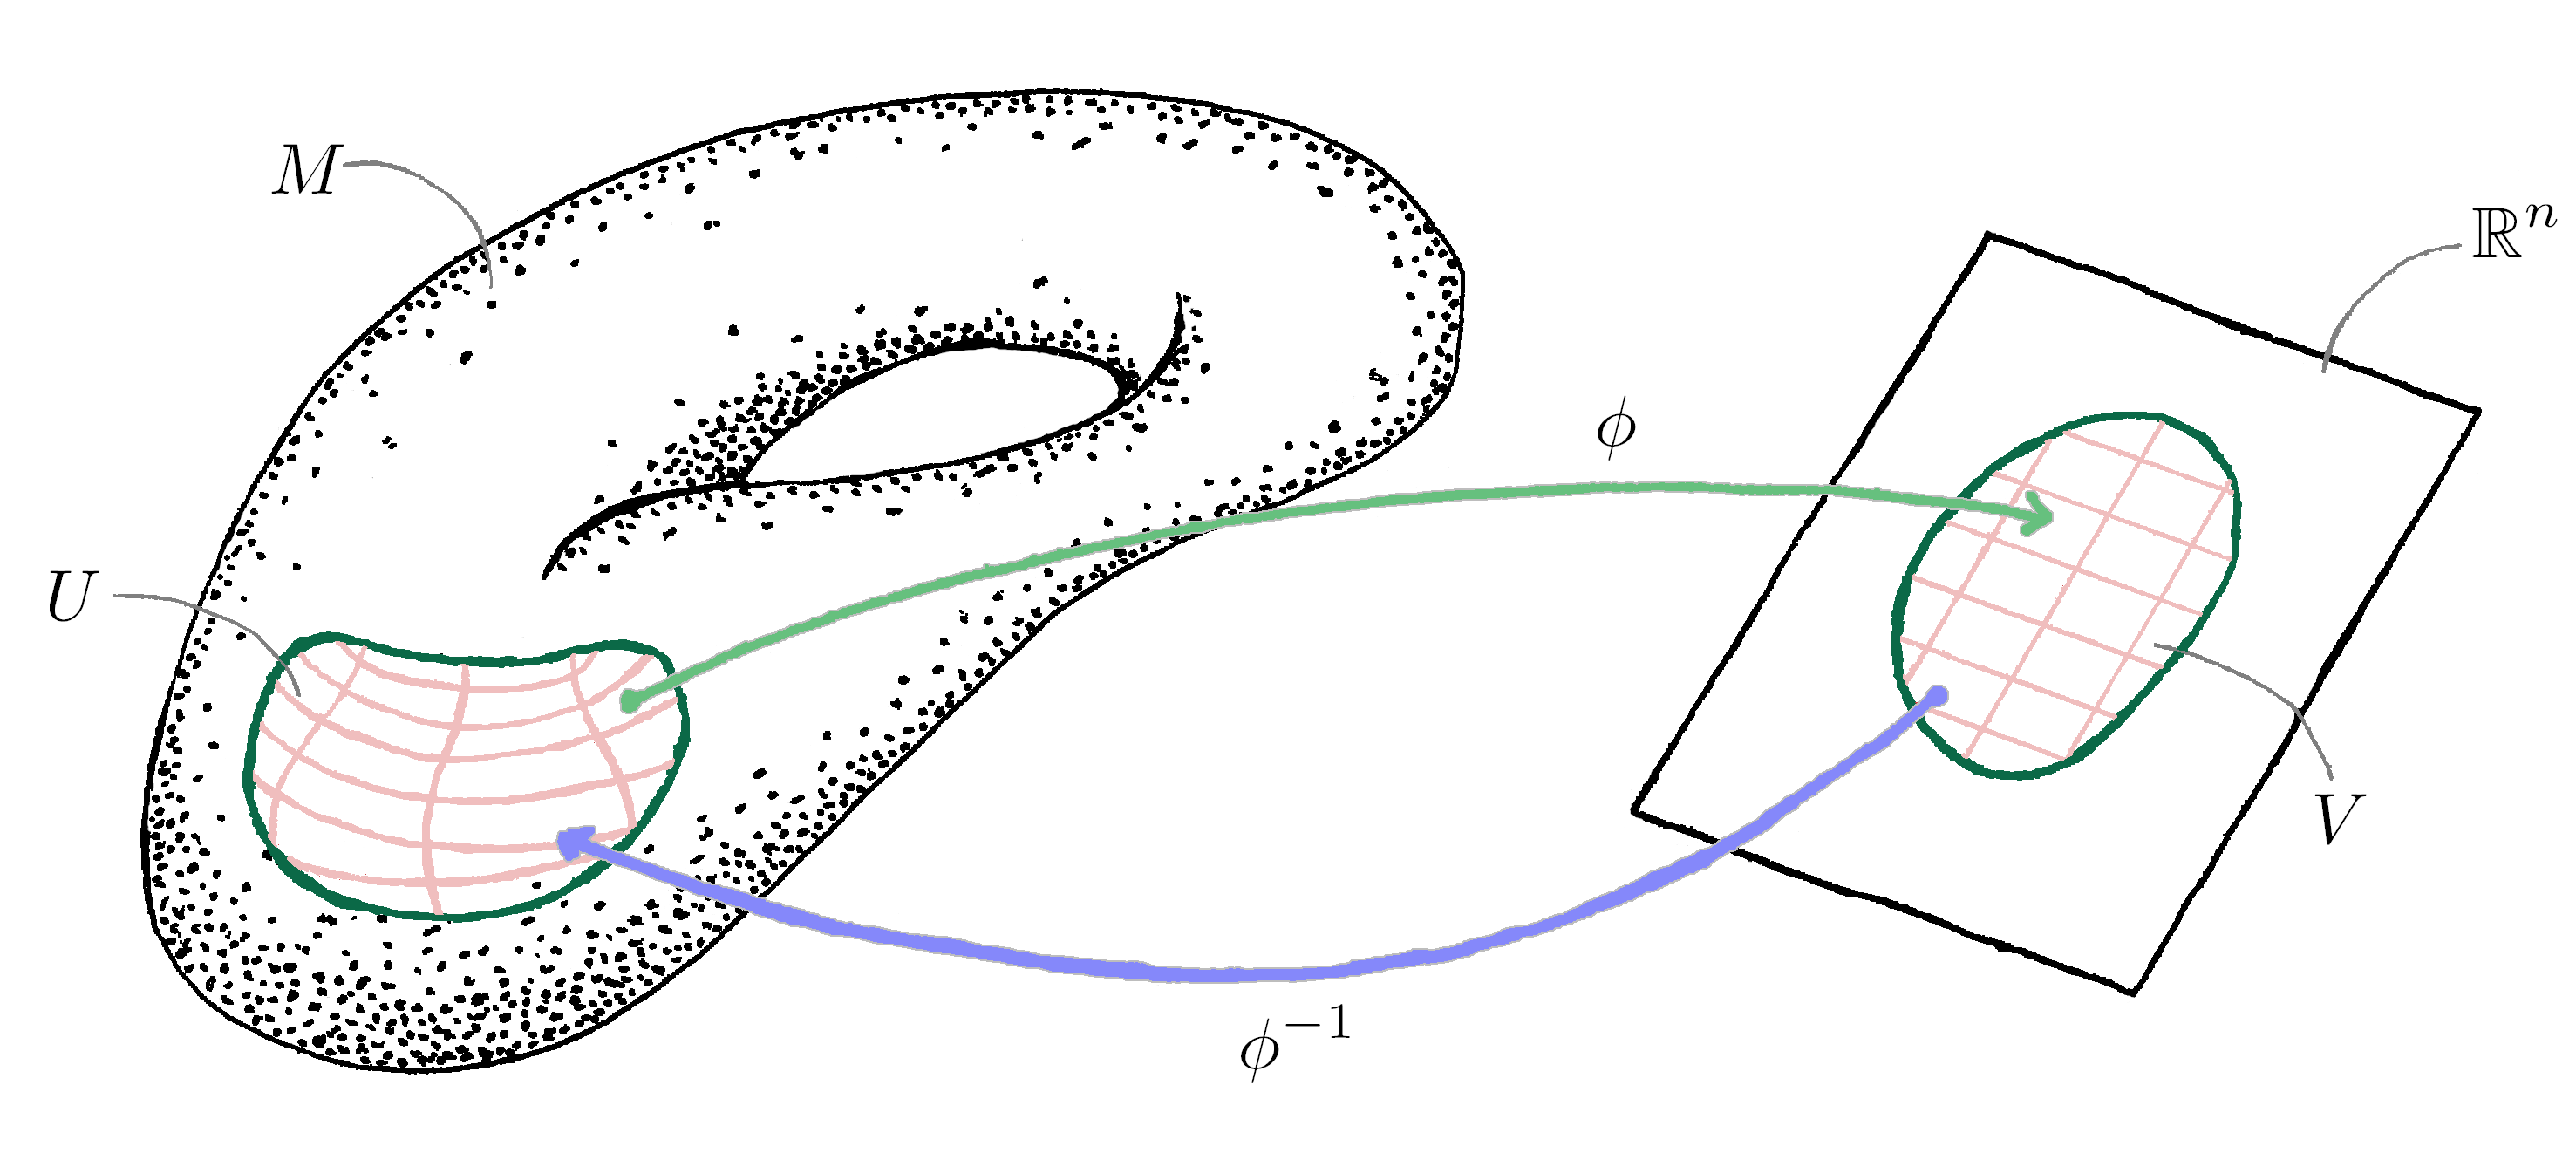
\includegraphics[scale=0.5]{figs/coord_patch/manifold_phi_inv.png}
\caption{The inverse of a chart $\phi$ provides $M$ with a local coordinate system. Coordinate lines in $V \subset \rR^n$ are mapped by $\phi^{-1}$ to continuous curves in $M$ which trace the local coordinate system on $M$.}
\label{coord_patch}
\end{figure}

(today upgrade definition of topological manifold to a smooth one)

We next describe what it means for a manifold to be \ul{smooth}. We use charts to interpret smoothness.

Given charts $\phi: U\to V$, $\theta: U' \to V'$ on $M$, assume $U\cap U' \neq \emptyset $. Then there $\exists h : \phi(U\cap U')\to \theta(U\cap U')$ such that the following diagram commutes

\begin{center}
\begin{tikzcd}[column sep=tiny]
& U\cap U' \ar[dl,"\phi \large|_{U\cap U'}"'] \ar[dr,"\theta \large|_{U\cap U'}"] & \\
\underset{\subset V \subset \rR^n}{\phi(U\cap U')}\ar[rr,"h"'] & & \underset{\subset V' \subset \rR^n}{\theta(U\cap U')}
\end{tikzcd}
\end{center}

$h:=\theta \large|_{U\cap U'}\circ \phi \large|_{U\cap U'}^{-1}$. Observe that $h$ is a homeomorphism between open sets in $\rR^n$. As a map of Euclidean spaces, it makes sense to ask: is $h$ smooth, i.e. infinitely differentiable? $h$ is called a ``transition function''.

\begin{defn}
An atlas $\{\phi_\alpha\}$ is said to be a \ul{smooth atlas} if all transition functions are smooth $(\cinf)$ with smooth inverses.
\end{defn}

(note smooth functions like $x^3$ don't necessarily have smooth inverses everywhere).

Two overlapping charts are said to be ``smoothly compatible'' if the corresponding transition function is smooth. 

Given a smooth atlas, we could expand the atlas by including all possible charts which are smoothly compatible with each other. So any smooth atlas can be expanded to a ``maximal $\cinf$ atlas''.

\begin{defn}
A smooth manifold is a topological manifold equipped with a maximal smooth atlas. Such a maximal atlas is called a ``\cinf structure''
\end{defn}

(question about uniqueness of maximal atlases - 28 different ones for \sph{7}, Milnor came up with an example. Exotic differentiable structures)
 
\ul{Remark} One of the benefits of a smooth structure is that it allows us to define an ambiguous  way whether `objects' defined on the manifold (e.g. functions) are smooth or not.

\ul{Examples} 
\begin{itemize}
\item Dim 0: one-point spaces (or disjoint unions of one point spaces). $\sph{0}=\{1,-1\}$. 
\item Dim 1: \rR or \sph{1}. (other manifolds with boundary but not defining that).
\item \ul{Dim 2} (theorem) Two families
\begin{itemize}
\item the ``orientable'' family, \sph{2}, $\tor{2}=\sph{1}\times \sph{1}$, $\tor{2}\underset{\text{connected sum}}{\#}\tor{2}$,  $\tor{2}\#\tor{2}\# \tor{2}$, $\ldots$ (connected sum is removing a disk from each and joining with a cylinder).
\item the ``non-orientable'' family: $\underbrace{\rpk{2} (\text{real projective space}), K (\text{Klein bottle})}_{\text{these don't live in }\rR^3}$, $\sph{2}$ with $n$ discs removed with $n$ mobius bands glued in.
\end{itemize}
\item In any dimension $\rR^n$ is a manifold with atlas consisting of a single chart $\{\mathrm{id}_{\rR^n}\}$. Ditto $\mnf (\cong \fF^{n^2})$. 
\item We also have an $n$-sphere $\sph{n}\subset \rR^{n+1}$. $\sph{n}=\{(x_1,\ldots,x_{n+1})\mid \sum\limits_{i=1}^{n+1}x_i^2=1\}$.
\end{itemize}

\section{Lecture 14 27/10/23}

To see that \sph{n} is a manifold we describe an atlas involving $2n+2$ charts. Take open hemispheres about the points $\pm e_1, \pm e_2, \ldots,\pm e_{n+1}$. We define a chart for each of these half spheres to $\rR^n = $ space orthogonal to $\pm e_i$ by projection (picture of projection). This is a smooth atlas as the transition functions, which are compositions of projections are clearly smooth maps. (There's also an atlas with just two charts, using stereographic projection from the poles. Messy exercise).

\ul{Exercise} If $M$ and $N$ are manifolds, show that $M\times N$ (with the product topology) is a also a manifold with dimension $\dim M +\dim N$.

\ul{Example} 2-torus $\tor{2}=\sph{1}\times \sph{1}$. 3-torus $\tor{3}=\sph{1}\times \sph{1}\times \sph{1}$, $n$-torus $\tor{n}=\sph{1}\times \ldots \times \sph{1}$. Tori are extremely important in the theory of Lie groups.  (they're abelian groups).

\begin{defn}
If $M^m$ (notation for dimension of a manifold) is a $\cinf$- manifold and $N\subset M$ is a subset equipped with the subspace topology (intersect open sets with subset) then $N$ is a dimension $n(<=m)$ \ul{submanifold} if for every $x\in N$ there is a chart $\phi:U\to V$ \ul{of M} with $x\in U$, such that $\phi(U\cap N)=\phi(U)\cap \left(\underset{\subset \rR^m=\rR^n \times\rR^{m-n}}{\rR^n\times \{0\}}\right)$. The restriction of charts taking this form to $N$ gives an atlas for $N$.
\end{defn}

\ul{Examples} \begin{itemize}
\item[i)] \sph{n} is a submanifold of $\rR^{n+1}$. 
\item [ii)] The equator $\sph{n-1}\subset \sph{n}$ is a submanifold of $\sph{n}$.
\item[iii)] $\sph{1}\times \{p\}\subset \sph{1}\times\sph{1}=\tor{2}$ is a circular submanifold of \tor{2}.
\end{itemize}

\ul{Remark} There are ways of detecting submanifolds which are easier than finding atlases.
 
\begin{thm}
(Whitney embedding theorem) Any smooth $n$-manifold can be $\underset{\text{(diffeomorphic)}}{\text{realised}}$ as a submanifold of $\rR^{2n}$. (No proof included)
\end{thm} 

\ul{Maps between manifolds}

\begin{defn}
A map of smooth manifolds $f:M\to N$ is \ul{smooth} if for every $x\in M$ and every chart $\theta:U'\to V'$ of $N$ with $f(x)\in U'$ and every chart $\phi:U\to V$ for $M$ with $x\in U$ and $f(U)\subset U'$, there is a \ul{smooth} map $\bar{f}$ making the following square commute:
\end{defn}

\begin{center}
\begin{tikzcd}
  U\subset M \arrow{d}{\phi} \arrow{r}{f\big|_U}
    & f(U)\subset N \arrow{d}{\theta\big|_{f(U)}} \\
  V \arrow{r}{\bar{f}}
&\theta(f(U)) \end{tikzcd}
\end{center}

\ul{Idea} $\bar{f}$ is the 'same' as $f$ just viewed through charts. Need to use charts here as smooth only makes sense in Euclidean spaces. 

\begin{defn}
A bijection of smooth manifolds $f:M\to N$ is a \ul{diffeomorphism} if it is smooth with smooth inverse.
\end{defn}

\begin{defn}
A \ul{Lie group} is a group $G$ which is also a smooth manifold for which the multiplication map $G\times G\to G$ and the inverse map $G\to G$ are both smooth.
\end{defn}
 
(Aside: Gromoll Meyer sphere $_{\gspk{1}}\slash ^{\gspk{2}} \backslash _{\gspk{1}}$ biquotient. Exotic sphere with non-negative curved)
 
\section{Lecture 15 06/11/23}

\ul{Previously}

\begin{itemize}
\item Manifold $M^n$ is a topological space locally $\cong \rR^n$. Charts give a way of doing calculus locally on a manifold. Transition functions from a smooth atlas give us a way of making the local calculus global: they guarantee that calculus in one chart agrees with that in any overlapping chart.
\item Smooth functions $f:M \to N$ are those which are smooth when viewed through charts.

\begin{center}
\begin{tikzcd}
  U\subset M \arrow{d}{\phi} \arrow{r}{f\big|_U}
    & f(U)\subset N \arrow{d}{\theta\big|_{f(U)}} \\
 V \arrow{r}{\bar{f}}
&W \end{tikzcd}
\end{center}
i.e. want $\bar{f}$ to be smooth for any suitable choice of charts in $M,N$.
\item Lie groups: this is a group $G$ which is also a $\cinf$ manifold s.t. multiplication $G\times G\to G$ \& inverse $G\to G$ are both \cinf.
\end{itemize} 

Consider a differentiable map $g:\rR^n\to \rR^m$. The derivative of $g$ is described by the Jacobian  matrix. Writing $g=(g_1,g_2,\ldots, g_m)$,

\[\pmqty{\pdv{g_1}{x_1} & \ldots & \pdv{g_1}{x_n}\\ 
\vdots & \ldots & \vdots \\ 
\pdv{g_m}{x_1} & \ldots & \pdv{g_m}{x_n} }\]

At some point $p\in \rR^n$ the Jacobian has "a rank" = max no of linearly independent rows/columns. (A result of linear algebra says that the row and column rank are the same.) For a differentiable map $f:M\to N$ the rank of $f$ at $p\in M$ is the rank of the Jacobian matrix $\bar{f}$ at the point corresponding to $p$ in $\rR^n$. 
\ul{NB} This concept of rank for maps between manifolds is well defined, i.e. is independent of the charts used to define $\bar{f}$. This is a consequence of the smooth atlas definition (smooth transition functions).

\begin{defn}
$f:M^m\to N^n$ a \cinf map, $m\geq n$.
\begin{itemize}
\item[a)] A point $p\in M$ at which (less than maximal) $\rank_{p}{f}<n$ is called a \ul{critical value} of $f$, and $f(p)$ is a \ul{critical value}.
\item[b)] A point $y\in N$ is a \ul{regular value} of $f$ if $\rank_{p}{f}=n$ (i.e. maximal) $\forall p \in f^{-1}(\{y\})$ (preimage of $y$).
\end{itemize}
\ul{Important convention}
Every point of $N$ which is \ul{not} in image of $f$ is declared to be regular.
\end{defn}

\begin{thm}
(The implicit Function Theorem - manifolds version).

If $y\in N$ is a regular value of $f:M^m\to N^n$ ($m\geq n$) a smooth map, then the pre-image $f^{-1}(\{y\})$ is a smooth submanifold of $M$ with dimension $m-n$. 

(No proof)
\end{thm}
 
This is particularly useful when $M=\rR^n$ or $M=\mnf (\cong \fF^{n^2})$.

e.g.

$f:\rR^n \to \rR$ defined by $f(x_1,x_2,\ldots, x_n)=\sum\limits_{i=1}^n x_i^2$. Then $f^{-1}(\{1\})=\sph{n-1}$. We conclude from IFT (2.1.11) that $\sph{n-1}$ is a manifold of dimension $n-1$ provided that $1$ is a regular value of $f$.  $\jac{f}=(\pdv{f}{x_1},\pdv{f}{x_2},\ldots,\pdv{f}{x_n})$ $=(2x_1,2x_2,\ldots,2x_n)$. This has rank $1$ unless $(2x_1,2x_2,\ldots,2x_n)=0$, but $0\not\in f^{-1}(\{1\})$, so this does not occur. So $1$ \ul{is} a regular value of $f$.

\ul{Applications to groups of matrices}

Firstly, since $\mnr\cong \rR^{n^2}$ and $\rR^{n^2}$ is trivially a manifold, $M_n(\rR^n)$ is a manifold. Next, observe that any open subset of a manifold is again a manifold under restriction of the topology and charts.

$\glnr = \{A\in \mnr \mid \det A\neq 0\}$. This is an open subset of $\mnr$ ($\glnr = \det ^{-1}(\rR \setminus \{0\})$. (preimage of an open set under a continuous function is open, $\rR \setminus \{0\}$ is open). $\therefore \glnr$ is a manifold of dim $n^2$. (Similar comments for \glnc and \glnh).

\section{Lecture 16 08/11/23}

Last time:

\begin{itemize}
\item \glnr is a manifold of dimension $n^2$. (because it's an open subset of $\mnr\cong \rR^{n^2}$. Similar comments for \glnc, \glnh .
\item Differentiable map $f:M^n\to N^n$, with $m\geq n$, then the rank of $f$ at $p\in M$ $\underset{\text{defn}}{=}$ rank of Jacobian map of $\bar{f}$ ($f$ viewed through chart, i.e. as a map between open subsets $\rR^m$, resp. $\rR^n$.
\item $y\in N$ is a regular value of $\rank_p f = n$ (maximal!) $\forall p \in f^{-1}(\{y\})$.
\item Implicit function theorem: if $y$ is a regular point, then pre-image $f^{-1}(\{y\})$ is a smooth submanifold of $M$ with dimension $m-n$.
\end{itemize}

\ul{Examples of Lie Groups}
\begin{itemize}
\item[(i)] $\gsln = \{A\in \mnr \mid \det A=1\}$. Consider $\det:\glnr\to \rR$. So $\gsln = \det^{-1}(\{1\})$.  By the IFT we will see that \gsln is a submanifold of \glnr with dimension $n^2-1$ and hence a Lie group since the multiplication and inversion in \gsln are the restrictions of the smooth multiplication and inversion in \glnr. We $\therefore$ need  to show that $1\in \rR$ is a regular value for $\det$, i.e. we need to show that the rank of $\det \neq 0$ at each $A\in \glnr$ with $\det A = 1$, i.e. the derivative at $A$ (in some direction through \glnr is non-zero). Consider the path $p(t)=(1-t)A$. $\det p(t) = (1-t)^n \det A = (1-t)^n$. $p(t)\in \glnr$ for $t$ small. Differentiating $\dv{t} \det \eval{p(t)}_{t=0}=\dv{t}\eval{(1-t)^n}_{t=0}=\eval{n(1-t)^{n-1}}_{t=0}=n\neq 0$.
Thus the rank of the $\det$ is maximal (i.e.$=1$), at every $A\in\gsln$ as required.
\item[(ii)] $\gson=\{A\in\mnr \mid AA^T=I_n\}$. Observe that $AA^T$ is symmetric, i.e. $(AA^T)^T=AA^T$. Let $S_n(\rR)=\{A\in \mnr \mid A \text{ is symmetric i.e. } A^T=A\}$. Notice that $S_n(\rR)\cong \rR^{\frac{1}{2}n(n+1)}$ as any element of $S_n(\rR)$ is determined by its upper/lower triangle of entries. So $S_n(\rR)$ is a manifold! 

Define $f:\underset{\cong \rR^{n^2}}{\mnr} \to \underset{\cong \rR^{\frac{1}{2}n(n+1)}}{S_n(\rR)}$, by $f(A)=AA^T$. ($f ``=" \bar{f}$)) Apply IFT to $f$. 

\ul{Claim} every element of $S_n(\rR)$ in $f^{-1}(\{I_n\})$ is a regular value of $f$. Choose $A,B \in \mnr$ and consider the path $A+tB\in \mnr$. Differentiating $f$ along this path at $t=0$: $df_A(B)$ (Deriv of $f$ at $A$ (i.e. $t=0$) in direction of $B$).
\begin{align*}
df_A(B)&=\dv{t}\eval{f(A+tB)}_{t=0}\\
&=\lim_{t=0} \frac{f(A+tB)-f(A)}{t}\\
&=BA^T+AB^T
\end{align*}
Calculation: exercise. Notice that $BA^T+AB^T$ is also symmetric! Thus $df_A:\mnr\to S_n(\rR)$. The claim follows if we can show $df_A$ is surjective (since $df_A$ is linear) for each $A\in f^{-1}(I_n)$. To see this: for any $C\in S_n(\rR) $ we can easily check that by setting $B=\frac{1}{2}CA$, we obtain $df_A(B)=C$. $\therefore$ by IFT $\gson =f^{-1}(\{I_n\})$ is a manifold of dimension $n^2-\frac{1}{2}n^2-\frac{1}{2}n=\frac{1}{2}n(n-1)$.

\end{itemize}

\section{Lecture 17 10/11/23}
Last time:

Showed \gson is a submanifold of \mnr of dimension $\frac{1}{2}n(n-1)$ using Implicit Function Theorem.

To show that \gson is a Lie group we simply observe that the multiplication and inverse operations agree with those (where defined) in \mnr, and hence are smooth.

\subsubsection{Tangent Spaces}

Consider a submanifold $M^m\subset \rR^n$. Let $p\in M$ and consider a smooth path $\gamma:(-\epsilon,\epsilon)\to M\subset\rR^n$ with $\gamma(0)=p$. (small picture of gamma in manifold, with velocity vector).

The velocity vector $\gamma'(0)$ is  a vector in $\rR^n$. Now consider the set of \ul{all} such paths $\gamma$. From this we get a set of velocity vectors $\subset \rR^n$. Intuitively it is clear that this set is an affine vector space, i.e. a vector space translated to the point $p$.

\begin{defn}
\begin{itemize}
\item[(a)] The \ul{tangent space} to $M\subset\rR^n$ to $p$, \tpm , is the set of velocity vectors to $M$ at $p$.
\end{itemize}
\end{defn}

\ul{Aim}: formulate an intrinsic notion of tangent space, i.e. not depending on a choice of embedding into some $\rR^n$.

\ul{Observation}: Given a path $\gamma$ through $p$ in $M$ \ul{as before}, and a differentiable function $f:M\to \rR$, consider the composition $f\circ \gamma:(-\epsilon,\epsilon)\to \rR$. This is differentiable. We can think of this derivative as a directional derivative of $f$ in the direction of $\gamma'(0)$. We can therefore identify velocity vectors $\gamma'(0)$ at $p$ with directional derivative operations, i.e. with differential operators. The point is that this makes as much sense for abstract manifolds as for submanifolds of $\rR^n$.

Denote the set of all \cinf real-valued functions on $M$ by  \cinfm. 

\begin{defn}
Given a smooth curve $\gamma(t)$ on $M$ with $\gamma(0)=p$, the \ul{tangent vector} to $\gamma$ at $p$ is a map $\gamma'(0):\cinfm \to \rR$ given by $\gamma'(0)(f)=\dv{t}\eval{f\circ \gamma(t)}_{t=0}$.
\end{defn}

Given a chart $\phi:\underset{\subset M}{U}\to \underset{\subset \rR^m}{V}$, we can use the standard coordinates $(x_1,x_2,\ldots, x_m)$ in $V$, $x_i :V\to \rR$, to obtain a local coordinate system in $M$, given by $(x_1\circ \phi, \ldots, x_m\circ \phi)$. For simplicity, we'll call these coordinates on $M$, $(x_1,\ldots, x_m)$.

Assume that $p\in U$ and $\phi(p)=0\in V\subset \rR^m$. In these coordinates we have $\gamma(t)=(\gamma_1(t),\ldots,\gamma_m(t))$, ($\gamma_i :(-\epsilon,\epsilon)\to \rR$) and $\therefore$

\begin{align*}
\dv{t}\eval{f\circ \gamma(t)}_{t=0}&=\dv{t}\eval{f(\gamma_1(t),\ldots,\gamma_m(t))}_{t=0}\\
&\underset{\text{chain rule}}{=}\sum_{i=1}^{m} \pdv{f}{x_i}(p)\gamma_i'(0)\\
&=\left(\sum_{i=1}^{m} \gamma_i'(0)\pdv{x_i}(p)\right) (f)
\end{align*}

where $\pdv{x_i}(p)$ is the tangent vector to the $x_i$ coordinate line at $p$, i.e. $(0,\ldots,0,\underset{i^{th} \text{ place}}{t},0,\ldots,0)$ in coords of U.

$\therefore \gamma'(0) = \sum_{i=1}^{m} \gamma_i'(0)\pdv{x_i}(p)$ $(*)$.

Observe that this only depends on the derivative of $\gamma$ at $p$.

\addtocounter{thm}{-2}
\begin{defn}
\begin{itemize}
\item[(b)] The \ul{tangent space} \tpm for any manifold $M$ is the set of velocity vectors (as defined above) to $M$ at $p$. The following is evident from $(*)$.
\end{itemize}
\end{defn}

\addtocounter{thm}{1}

\begin{lemma}
\tpm is a vector space of dimension $=\dim M$, and given local coordinates system $(x_1,x_2,\ldots, x_m)$ around $p$, a basis for \tpm is given by 
\[\{\pdv{x_1}(p),\ldots, \pdv{x_m}(p) \}\]
\end{lemma}

Notice that \tpm is independent of local coord systems, since tangent vectors themselves are indep. of local coords.

\section{Lecture 18 13/11/23}

Last time:

\begin{itemize}
\item tangent vector to a manifold $M$ at $p\in M$ is a directional differentiation operator at $p$. (Acting on smooth functions $M\to \rR$).
\item Tangent space \tpm is the set of all tangent vectors at $p$.
\item $\tpm = \operatorname{span}\{\pdv{x_1}(p),\ldots, \pdv{x_n}(p) \}$, where $(x_1,x_2,\ldots, x_n)$ is any local coordinate system on $M$ about $p$, and $\pdv{x_i}$ are the usual partial differentiation operations.
\end{itemize}

The collection of all tangent spaces $\bigcup\limits_{p\in M} \tpm^n$ has the structure of a manifold (non-compact!) of dimension $2n$. This is denoted $\tm$ and is called the "tangent bundle".

\ul{Examples}
\begin{itemize}
\item[(i)] $\tqn{p}{\rR^n}\cong \rR^n$. Consider a path $\gamma(t)=p+vt$ for some $v\in \rR^n$, $\gamma'(0)=v$. Thus the corresponding tangent (velocity) vector is $v$. 

Alternatively natively consider $\dv{t}\eval{f(p+vt)}_{t=0}$. If $v=\sum \lambda_i e_i$ then this is 
\begin{align*}
&\sum \pdv{f}{x_i}\lambda_i \quad \text{by the chain rule.}\\
&=\left(\sum \lambda_i \pdv{x_i}\right)(f)
\end{align*}
So $\sum \lambda_i \pdv{x_i}$ is the tangent vector corresp to $v=\sum \lambda_i e_i$. The correspondence $\tqn{p}{\rR^n}\cong \rR^n$ is precisely $\sum \lambda_i \pdv{x_i} \leftrightarrow \sum \lambda_i e_i$.

\item[(ii)] $\tqn{A}{\mnr} \cong \mnr$. (Essentially a special case of (i)). Consider a path $\gamma(t)=A+tB$ for some $B\in \mnr$. Clearly $\gamma'(0)=B$. Alternatively, consider $\dv{t}\eval{f(A+tB)}_{t=0}$. Let $v_{ij}:\mnr \to \rR$ be the function which picks out the $(i,j)^{th}$ entry. Standard coordinates on \mnr.
\begin{align*}
\dv{t}f(A+tB)&\underset{\text{chain rule}}{=}\sum_{i,j} \pdv{f}{v_{ij}}b_{ij}\\
&=\left(\sum_{i,j}\pdv{f}{v_{ij}}b_{ij}\right)(f)
\end{align*}
So $\sum_{i,j}\pdv{f}{v_{ij}}b_{ij}$ is our tangent vector which we can identify with matrix $(b_{ij})=B$.

\item[(iii)]  $S_n(\rR)=\{(\nn) \text{ symmetric matrices }\}\cong \rR^{\frac{1}{2}n(n+1)}$. Same argument as in (ii) shows that $\tqn{A}{S_n(\rR)}\cong \S_n(\rR)$
\item[(iv)]  $\tqn{A}{\glnr}\cong \mnr$. We can see this two ways:
\begin{itemize}
\item[(a)] Since \glnr is an open subset of \mnr
\item[(b)] using same argument as (ii) after noting that for $A\in \glnr, B\in \mnr$, the path $A+tB$ lies in \glnr for $t close to 0$.
\end{itemize}
\end{itemize}

\begin{defn}
Given a differentiable map $f:M^n\to N^n$, the derivative of $f$ at $p\in M$, $\dfp$ is a map $\dfp:\tpm\to\tqn{f(p)}{N}$ given by $\dfp(X)=X(g\circ f) \forall g\in \cinfn{N}, \forall X\in \tpm$.
\end{defn}

\ul{Idea} Given a differentiable path $\gamma(t)$ through $p\in M$, $f(\gamma(t))$ is a differentiable path through $f(p)$ in $N$. If $X\in\tpm$ is the tangent vector $\gamma'(0)$ then $\dfp(X)$ is the tangent vector corresp. to $f(\gamma(t))$ at $f(p)$. (picture of path and image of path, tangent vectors etc)

\begin{lemma}
\dfp is a linear map.
\end{lemma} 
\begin{proof}
Trivial, from definition of \dfp.
\end{proof}

The individual derivatives \dfp can be assembled into a 'total' derivative $\df:\tm\to\tn{N}$ between tangent bundles.

\ul{Remarks}
\begin{enumerate}
\item Given coordinate systems about $p$ and $f(p)$ we obtain bases for \tpm and \tqn{f(p)}{N} and with respect to these bases, \dfp is given by a matrix. This is just the usual Jacobian matrix.
\item We can now re-interpret the notions of regular/critical points in terms of \dfp being surjective/ not surjective.
\item Previously we saw a map $f:\mnr \to S_n(\rR)$, $f(A)=AA^T$ we decided that \dfq{A} is a map $\mnr \to S_n(\rR)$. In reality $\dfq{A}:\underset{\cong\mnr}{\tqn{A}{\mnr}}\to \underset{\cong S_n(\rR)}{\tqn{AA^T}{S_n(\rR)}}$
\end{enumerate}

\ul{Vector Fields}
\begin{defn}
A (tangent) vector field on a smooth manifold $M$ is a choice of tangent vector at each $p\in M$, i.e. a rule which assigns $X(p)\in\tpm$ to each $p\in M$.
\end{defn}

Given a coord system $\xonen$ locally on $U\subset M$. We can express (locally) a vector field on $U$ as $\sum \lambda_i(p)\pdv{x_i}(p)$. Here $\lambda_i:U\to \rR$. We say the vector field is \ul{smooth} if the $\lambda_i$ are all smooth. The vector field is globally smooth (which we will assume from now on) if it is smooth in every chart. This is a well-defined concept, as the notion of smoothness is the same viewed from any charts in a smooth atlas.

\section{Lecture 19 15/11/23}

Last time:

\begin{itemize}
\item A tangent vector field on manifold $M$ is a choice of tangent vector in \tpm for each $p \in M$. This choice is assumed to be smoothly varying with $p$.
\end{itemize}

From now on we will use the term vector field to mean tangent vector field.

\ul{Remark}: A flow on $M$ is a one-parameter, smoothly varying, family of diffeomorphisms $M \to M$. (for example, flow of air around the earth) (TODO: insert figure of flow here). Differentiating a flow gives a vector field. Conversely,  vector field can be integrated to give a flow.

\subsubsection{Lie Algebras}

Let $X, Y$ be vector fields on $M$.

\begin{defn}
The Lie bracket of $X$ and $Y$, denoted $[X, Y]$ is\footnote{multiplication on the R.H.S. makes sense if vector fields are interpreted as differential operators.}
\[ [X, Y] = XY - YX. \]
\end{defn}

\begin{lemma}
$[X, Y]$ is a vector field on $M$. (ie it is a first order differential operator, not second order)
\end{lemma} 

\begin{proof}
Let $f \in \cinfn{M}$. So $XY(f) = X(Yf)$ etc. Note, $Yf \in \cinfn{M}$. With respect to a local coordinate system $(x_1,x_2,\ldots, x_n)$ we have
\[ X = \sum_i \lambda_i \pdv{x_i}, \quad Y = \sum_i \mu_i \pdv{x_i}, \]
for some $\lambda_i , \mu_i \in \cinfn{M}$.

Computing, we have
\begin{align*}
XYf - YXf &=  \sum_{i,j} \left(\lambda_i \pdv{\mu_j}{x_i} \pdv{f}{x_j} 
                       - \mu_j \pdv{\lambda_i}{x_j} \pdv{f}{x_i}\right) \\
          &+ \sum_{i,j} \lambda_j\mu_j\left( \pdv{^2f}{x_i\partial x_j}
           - \pdv{^2f}{x_j\partial x_i} \right).
\end{align*}
But the second partial derivatives commute.
\[ \therefore [X, Y](f) = \sum_{i,j} \left(\lambda_i \pdv{\mu_j}{x_i} \pdv{f}{x_j} 
                       - \mu_j \pdv{\lambda_i}{x_j} \pdv{f}{x_i}\right). \]
\[ \therefore [X, Y] = \sum_{i,j} \left(\lambda_i \pdv{\mu_j}{x_i} \pdv{x_j} 
                       - \mu_j \pdv{\lambda_i}{x_j} \pdv{x_i}\right). \]
\end{proof}

\ul{Remark}: This has a nice interpretation in terms of flows and is sometimes called a Lie derivative. One can define a way to push/pull $Y$ along the flow of $X$ and differentiate it, this gives a notion of differentiating $Y$ with respect to $X$. We won't explore this further here.

\begin{lemma}
The Lie bracket has the following properties:
\begin{enumerate}
\item It is bilinear.
\item It is anti-symmetric (ie $[X, Y] = - [Y, X]$).
\item It satisfies the "Jacobi identity":
\[ [[X, Y], Z] + [[Z, X], Y] + [[Y, Z], X] = 0. \]
\end{enumerate}
\end{lemma}

\begin{proof}
Properties 1 and 2 are trivial. For 3 we can simple write out each term and add. ie
$[[X, Y], Z] = [XY - YX, Z] = XYZ - YXZ - ZXY + ZYX$ etc. (exercise!)
\end{proof}

We now focus on vector fields on Lie groups.

For $g \in G$ ($G$ a Lie group) we have diffeomorphisms $L_g:G\to G$ given by $L_g(h) = gh$ (ie by left multiplication) and $R_g:G\to G$ given by $R_g(h) = hg$. We will concentrate on $L_g$ but everything will hold true for $R_g$ also. We have $dL_g : T_hG \to T_{gh}G$ for any $h \in G$.

\begin{defn}
A vector field $X$ on $G$ is left-invariant if $dL_g(X) = X \,\, \forall g \in G$. ie $dL_g(X_h) = X_{gh} \,\, \forall g, h \in G.$
\end{defn}
A similar definition can be made for right-invariance.

\begin{lemma}
There is a bijection between the set of left invariant vector fields (LIVF) and $T_eG$.
\end{lemma}

\ul{Remark}: Since the set of LIVFs is a vector space (if $X, Y$ are LIVFs then trivally so is $\lambda X + \mu Y$) this bijection is actually a linear ismorphism.

\begin{proof}
For any $v\in T_eG$ we can construct a LIVF by "left propagation". ie let $X_g = dL_g(v) \,\, \forall g\in G$. The resulting field $X$ is left invariant:
\begin{align*}
dL_g(X_h) &= dL_g \circ dL_h(v) & \\
&= d(L_g \circ L_h)(v) & \mbox{(by the chain rule)} \\
&= dL_{gh}(v) &\\
&= X_{gh}.
\end{align*}
This gives a map $T_eG \to \{LIVFs\}$. This map is trivally injective. Observe that there is an inverse map $X \mapsto X_e \in T_eG$. Therefore the map is a bijection.
\end{proof}

\begin{lemma}
If $X, Y$ are LIVFs, then $[X, Y]$ is a LIVF.
\end{lemma}

\begin{proof}
We begin by making the following claim: Let $f\in \cinfn{G}$. $X$ is left invariant $\iff (Xf)\circ L_g = X(f\circ L_g).$

\begin{center}
\begin{tikzcd}
G \ar[dr, "f \circ L_g"] \ar[r, "L_g"] & G \ar[d, "Xf"] \\
& \rR
\end{tikzcd}
\end{center}
To see this, suppose $p(t)$ is a $C^\infty$ path in $G$ with $p(0) = e, p'(0) = X_e.$ Then $X$ is left invariant $\iff X_h = \frac{d}{dt}hp(t)|_{t=0} \,\, \forall h \in G.$
\begin{align*}
\implies (Xf) \circ L_g(h) &= (Xf)(gh) & \\
&= X_{gh}(f) & \mbox{(as $X$ is left invariant)} \\
&= \dfrac{d}{dt}f(ghp(t))|_{t=0}. &
\end{align*}

Compare this with:
\begin{align*}
X(f\circ L_g)(h) &= (X_h)(f\circ L_g) & \\
&= \dfrac{d}{dt} (f\circ L_g)(hp(t))|_{t=0} & \mbox{(as $X$ is left invariant)} \\
&= \dfrac{d}{dt}f(ghp(t))|_{t=0}. &
\end{align*}
as before. So $(Xf)\circ L_g = X(f\circ L_g)$ (To be continued next lecture...)
\end{proof}


\section{Lecture 20 17/11/23}

Last time:

\begin{itemize}
\item A $X$ is a (tangent) vector field on Lie group $G$, then $X$ if left-invariant (LI) if, for all $g \in G$, $dL_g(X) = X$ where $L_g:G\to G$, $L_g(h) = gh$ for all $h\in G$ and $dL_g(X) = X$ means $dL_g(X_h) = X_{gh}$.

\item (2.3.5) There exists a bijection $T_eG\to $\{{LIVFs on G}\} given by "left propagation", ie for $v\in T_eG$ $X_h := dL_h(v) \,\, \forall h \in G$.

\item (2.3.6) If $X, Y$ are LI then so is $[X, Y]$.
\end{itemize}

\begin{proof} (2.3.6 continued)
Previously, we had made the following claim: For $f\in \cinfn{G}$, $X$ is left invariant if and only iff the following holds:
\[ (Xf)\circ L_g = X(f\circ L_g). \label{claim2.3.6} \tag{$\circledast$} \]

($\Longrightarrow$) was prove lasted time.

($\Longleftarrow$) Assume $(Xf)\circ L_g = X(f\circ L_g)$ holds. Then for any $h\in G$,
\[ (Xf)\circ L_g(h) = (Xf)(gh) = X_{gh}f. \]
Therefore, $X_{gh}f = X_h(f\circ L_g)$. By definition of the derivative map (2.2.4) we have
\[ X_h(f\circ L_g) = dL_g(X_h)(f). \]
Therefore,
\[ X_{gh}f = dL_g(X_h)(f), \quad \forall f \in \cinfn{G}. \]
Hence, $X_{gh} = dL_g(X_h)$, ie $X$ is LI. This proves the claim.

Now to prove 2.3.6, consider the following:
\begin{align*}
([X, Y]f)\circ L_g &= (X(Yf) - Y(Xf))\circ L_g, & \\
&= X(Yf)\circ L_g - Y(Xf)\circ L_g, & \mbox{(trivially)} \\
&= X((Yf)\circ L_g) - Y((Xf)\circ L_g) & \mbox{(by \ref{claim2.3.6})} \\
&= X(Y(f\circ L_g)) - Y(X(f\circ L_g)) & \mbox{(by \ref{claim2.3.6})} \\
&= (XY)(f\circ L_g) - (YX)(f\circ L_g) \\
&= [X, Y](f\circ L_g)
\end{align*}
Hence, $([X, Y]f)\circ L_g = [X, Y](f\circ L_g)$ and so, by the claim made at the start of the proof, we conclude that $[X, Y]$ is LI.
\end{proof}

Combining (2.3.5) nd (2.3.6) we immediately deduce:

\begin{cor}
Restricting the Lie bracket operation from \{LIVFs on $G$\} to $T_eG$ gives a map
\[ [\cdot , \cdot]: T_eG \cross T_eG \to T_eG, \]
which is bilinear, anti-symmetric and satisfies the Jacobi identity.
\end{cor}

\begin{defn}
\begin{enumerate}
\item A Lie algebra consists of a vector space $V$ over a field \fF, together with an operation $[\cdot , \cdot]:V\cross V \to V$ which is bilinear, anti-symmetric and satisfies the Jacobi identity.

\item The Lie algebra $\mathfrak{g}$ of a Lie group $G$ is $T_eG$ equipped with the operation $[\cdot , \cdot]$ from 2.3.7.
\end{enumerate}
\end{defn}

\ul{Remark:} The Lie bracket captures, in an infinitesimal and nonobvious way, the group structure of $G$.

\begin{obs}
In general, the ``multiplication" map $[\cdot ,\cdot]$ in a Lie algebra is not associative.
\end{obs}

If $[\cdot ,\cdot]$ was associative then $[[X, Y], Z] = [X, [Y, Z]]$. Then, by anti-symmetry we have $[[X, Y], Z] + [[Y, Z], X] = 0$. But the Jacobi identity tells us that
\[ [[X, Y], Z] + [[Y, Z], X] = -[[Z, X], Y] \]
which is non-zero in general.

\subsection*{Examples of a Lie algebras}

\begin{enumerate}
\item Let $V$ be any vector space and set $[v, w] = 0$ for all $v, w \in V$. Then $(V, [\cdot, \cdot])$ is a Lie algebra. Note, in this special case $[\cdot, \cdot]$ is associative.

\item On $M_n(\fF)$ define the commutator $[A, B] = AB - BA$. Then $(M_n(\fF), [\cdot, \cdot])$ is a Lie algebra.

\item Let $M$ be a smooth manifold and let $\Gamma (M)$ be the (real) vector space of all (tangent) vector fields on $M$. The Lie bracket $[X, Y] = XY - YX$ makes $\Gamma (M)$ into a Lie algebra. Note that this object is infinite dimensional.
\end{enumerate}

We have seen that $T_eGL_n(\rR) \cong M_n(\rR)$. Therefore, as a vector space, $\mathfrak{gl}_n(\rR) \cong M_n(\rR)$. What is the Lie bracket in this case?

\begin{thm}
The Lie bracket operation on $\mathfrak{gl}_n(\rR)$ is just $[A, B] = AB - BA \in M_n(\rR)$.
\end{thm}

\begin{proof}
See moodle! Here is the main idea:

Corresponding to $A$ and $B$ we have paths through $\cin$ in $GL_n(\rR)$, parameterised by $s$ and $t$ respectively. By left translation $(L_g)$ by elements close to $\cin$, we can create a ``mesh" of paths surrounding "\cin" by translating one of these paths along the other. This gives us a local 2-dimensional ``slice" around $\cin$ parameterised by $(s, t)$. We can compute second derivatives of $f\in \cinfn{GL_n(\rR)}$ with respect to the parameters. This allows us to identify the Lie bracket operation. (TODO: insert figure of coordinate patch construction around identity)
\end{proof}

\section{Lecture 21 20/11/23}
\ul{Last time}:
\begin{itemize}
\item Lie algebra is a vector space $V$ equipped with an operation $\comm{\cdot}{\cdot}$, $\comm{\cdot}{\cdot}:V\times V\to V$ s.t. $\comm{\cdot}{\cdot}$ is 
\begin{enumerate}
\item[i)] bilinear
\item[ii)] antisymmetric
\item[iii)] satisfies the Jacobi identity
\end{enumerate}


( In general $\comm{\cdot}{\cdot}$ is not associative) 

e.g. $\{\cinf $ vector fields on a manifold $\}$ is a Lie algebra under standard Lie bracket operation. 

e.g. $G$ a Lie group, then $\{LIVF\}$ is a Lie bracket under standard Lie bracket. This restricts to give a map $\comm{\cdot}{\cdot}:\tqn{e}{G}\times \tqn{e}{G}\to \tqn{e}{G}$, $(\tqn{e}{G}, \comm{\cdot}{\cdot})$ is the Lie algebra of $G$.

\item The general linear group $\glnr$ has Lie algebra $(\underset{=\tqn{e}{\glnr}}{\mnr}, \ecomm)$ where $\comm{A}{B}=\underbrace{AB-BA}_{\text{difference of matrix products}}$ for any $A,B\in \mnr$.

Same argument for \glnc or \glnh.

(an aside - if we think of \glnh as an abstract object, not as linear maps, we don't have to worry about the left/right multiplication issue, we can do left or right multiplication of matrices)
\end{itemize}

\begin{cor}
The Lie bracket operation for the other matrix groups (which are all Lie subgroups of \glnff) is just the restriction of that for $\glnr$ to the appropriate space of matrices, i.e. the Lie bracket of matrix groups is just the matrix commutator.
\end{cor}

\begin{thm}
The Lie algebra of \gon is 

\[\left(\underbrace{\{A\in \mnr \mid \underset{\text{skew-symmetric matrices}}{A^T=-A}\}}_{=\tqn{e}{\gon}}, \ecomm\}\right)\]
\end{thm}
\begin{proof}
Consider a \cinf path $A(t)$ in \gon with $A(0)=I_n$. We have $A(t)A^T(t)=I_n$ (by orthogonality).

$\therefore \dv{t}AA^T\underset{\text{product rule}}{=} A'A^T+AA'^T=0$.

At $t=0$ we obtain $A' + A'^T=0$, i.e. $A'^T=-A'$. So $A'\in \underset{\text{skew-symmetric matrices}}{\operatorname{SSym}_n(\rR)}$, i.e. $\lgon=\tqn{e}{\gon}\subset \operatorname{SSym}_n(\rR)$.

Conversely, $E_{ij}$ be the $(\nn)-$matrix with $1$ in position $(i,j)$ and $0$s elsewhere.

Observe that $\{E_{ij}-E_{ji}\}_{i\neq j}$ is a basis for $\operatorname{SSym}_n(\rR)$.

It suffices to find a path for each $(i,j)$, $i\neq j$ in \gon through $I_n$ with derivative $E_{ij}-E_{ji}$ at $I_n$.

Set $\gamma_{ij}=I_n+\sin(t)(E_{ij}-E_{ji})+(-1+\cos(t))(E_{ii}-E_{jj})$. Notice that $\gamma'_{ij}(0)=E_{ij}-E_{ji}$.

To see that $\gamma_{ij}(t)\in \gon$ (actually $\in \gson$ since \gon has two components, and we're in the identity component), we re-write in matrix form 

% without any indices this is fine
%\[\pmqty{\dmat{
%\dmat{1,1,\ddots,1},
%\mqty{\cos(t) & & & &\sin(t)\\
% & 1 & & & \\
%  &  &\ddots & & \\
%   &  & & 1 & \\
%   -\sin(t) & & & &\cos(t)
%},
%\dmat{1,1,\ddots,1}
%}
%}.\]

% this is a bit of a hack job - there's probably a more sensible way to do this
\[\mqty{
\mqty{i\\ {}\\ {}  \\ {}  \\ j} &
\pmqty{
\mqty{\dmat{1,1,\ddots,1}} & &\\
{}& \mqty{\cos(t) & & & &\sin(t)\\
 & 1 & & & \\
  &  &\ddots & & \\
   &  & & 1 & \\
   -\sin(t) & & & &\cos(t)
} &{}\\
{}&{} & \mqty{\dmat{1,1,\ddots,1}}
} \\
& \mqty{\quad i & \quad & \quad & \quad & \quad j}
}.\]

Since the rows of this matrix form an orthonormal set, we see by 1.2.5 that this matrix is orthogonal $\forall t$. (Actually this matrix represents a rotation in the plane $\mbox{Span}\{e_i,e_{j}\}$ through angle $t$.) 
\end{proof}

Similar arguments show:

\begin{thm}
The Lie algebra of \gun is 
\[\lgun = \{A\in \mnc \mid \underset{"skew Hermitian"}{\bar{A}^T=-A}\},\] 
and the Lie algebra of \gspn is 
\[\lgspn = \{A\in \mnh \mid \bar{A}^T=-A\},\]
both with matrix commutator as Lie bracket.
\end{thm}

\begin{cor}
\begin{align*}
& \dim \gon = \frac{1}{2}n(n-1)\\
& \dim \gun = n^2\\
& \dim \gspn = 2n^2+n
\end{align*}
\end{cor}

\begin{proof}
$\dim \gon = \dim \lgon = \dim \operatorname{SSym}_n(\rR)$.

A skew symmetric matrix is determined by the entries above the diagonal. There are 
\[\frac{1}{2}\left(\underset{\text{total no. of entries}}{n^2}- \underset{\text{no. of entries on diagonal}}{n^2}\right)\]
(all diag entries $=0$)

For \lgun, the diagonal entries must be pure imaginary. Off the diagonal, each entry determines two real nos. Overall we have 

\[\frac{1}{2}\left(\underset{\text{if diagonal entries } = 0}{2n^2-2n}\right) + \underset{\text{add back } n \text{for imaginary entries on diagonal}}{n}\]

$=n^2-n+n=n^2$.

In symplectic case, we have four real numbers for each entry, but diagonal entries must be pure imaginary (determined by three real nos) 
$\therefore \dim\lgspn= \frac{4n^2-4n}{2}+\underset{\text{diagonal entries}}{3n}=2n^2-2n+3n=2n^2+n $
\end{proof}

\section{Lecture 22 22/11/23}
\ul{Previously}:

\begin{itemize}
\item Lie bracket of matrix groups is the matrix commutator. $\comm{A}{B}=AB-BA$. So identifying the Lie algebra just requires identifying the tangent space at the identity \teg.
\item \glnr has Lie algebra $\lglnr=(\mnr, \ecomm)$, $\lgon=\{\text{skew symmetric matrices}, \ecomm\}$, $\lgun=(\{A\in\mnc \mid \bar{A}^T=-A \},\ecomm)$, $\lgspn=\ldots$. This leaves \gsln and \gsun. (As $\gon\underset{\text{topologically}}{\cong} \gson \amalg \gson$, we get $\lgson=\lgon$
\end{itemize}

For \gsln and \gsun we need a lemma:

\begin{lemma}
Suppose $A(t)$ is a \cinf path of matrices in \mnf such that $A(0)=I_n$. Then $\dv{t}\eval{\det A(t)}_{t=0}=\tr A'(0)$.
\end{lemma}

\begin{proof}
Recall that 
\[\det A = \sum_{\sigma\in S_n} \operatorname{sign}(\sigma) \prod_{i=1}^n a_{i \sigma(i)} \]
($S_n=$ symmetric group, i.e. permutations of $\{1,\ldots,n\}$, $A=(a_{ij})$)

Each term of sum, when differentiated gives an expression (product rule)
\[a'_{1\sigma(1)}a_{2\sigma(2)}\cdots a_{n\sigma(n)}+a_{1\sigma(1)}a'_{2\sigma(2)}\cdots a_{n\sigma(n)}+\ldots +a_{1\sigma(1)}a_{2\sigma(2)}\cdots a'_{n\sigma(n)}\]
At $I_n$, $a_{ij}=\delta_{ij}$, so this gives 
\[\dv{t}\eval{\det A(t)}_{t=0}=a'_{11}+a'_{22}+\ldots +a'_{nn} =\tr A'(0) \]
as all terms $a_{ij}$ with $i\neq j$ vanish. 
\end{proof}

\begin{thm}
As vectors spaces 
\begin{align*}
\lgslnr & =\{A\in \mnr \mid \tr A=0\}\\
\lgsun & =\{A\in \lgun \mid \tr A=0\}=\{A\in\mnc \mid \bar{A}^T=-A, \tr A=0\}.
\end{align*}
\end{thm}

\begin{proof}
The condition $\det A=1$ in the definitions of both \gsln and \gsun differentiate at $I_n$ to give $\tr A=0$ (by 2.3.15).
\end{proof}

A linear map of Lie algebras $f:\mathfrak{g}\to \mathfrak{h}$ is a \ul{Lie algebra homomorphism} if $f(\commg{u}{v})=\comml{f(u)}{f(v)}{h}$, $\forall u,v \in \mathfrak{g}$.

\begin{thm}
A smooth homomorphism of Lie Groups $\theta:G\to H$ induces a Lie algebra homomorphism $\dgq{\theta}{e}:\mathfrak{g}\to \mathfrak{h}$.
\end{thm}

\begin{proof}
Consider $u,v \in \mathfrak{g}$ and corresponding paths $\theta(t)$, $\psi(s)$ s.t. $\phi'(0)=u$, $\psi'(0)=v$. (picture).

Let $f\in \cinfn{H}$, so $f\circ \theta \in \cinfn{G}$. If $U$ and $V$ extend $u,v$ to LIVFs we have 
\[\dgq{\theta}{e} (V_g) (f) = \dv{s} \eval{f(\theta \circ \L_g \circ \psi(s))}_{s=0}\] 
by the definition of derivatives (2.2.4).

Then 
\begin{align*}
\eval{\dg{\theta}(U) \dg{\theta}(V) (f)}_{e_H}&=\dv{t}\eval{\dgq{\theta}{\phi(t)} (V_{\phi(t)}) (f)}_{t=0}\\
&=\pdv{}{t}{s}\eval{f(\theta\circ L_{\phi(t)}\circ \psi(s))}_{s=t=0}\\
&=\pdv{}{t}{s}\eval{f(\theta(\phi(t)\psi(s)))}_{s=t=0}
\end{align*}
So 
\[\commp{\dg{\theta}(U)}{\dg{\theta}(V)}{e_H}(f)=\pdv{}{t}{s}\eval{\left[f\circ\theta(\phi(t)\psi(s))-f\circ\theta(\psi(s)\phi(t))\right]}_{s=t=0}\]
Compare 
\[V_g(f\circ\theta)=\dv{s}\eval{f\circ\theta(g\psi(s))}_{s=0}\]
to 
\[\eval{UV(f\circ\theta)}_{e_G}=\pdv{}{t}{s}\eval{f\circ\theta(\phi(t)\psi(s))}_{s=t=0}\]

\begin{align*}
\therefore \eval{\dg{\theta}(\comm{U}{V})(f)}_{e_H} &=\eval{\comm{U}{V}(f\circ\theta)}_{e_H} \\
&= \eval{UV(f\circ\theta)}_{e_G}-\eval{VU(f\circ\theta)}_{e_G}\\
&= \pdv{}{t}{s}\eval{\left[f\circ\theta(\phi(t)\psi(s))-f\circ\theta(\psi(s)\phi(t))\right]}_{s=t=0}\\
&= \commp{\dg{\theta}(U)}{\dg{\theta}(V)}{e_H}(f) \quad \text{from above}
\end{align*}
\end{proof}

A \ul{Lie group isomorphism} is an isomorphism of Lie Groups which is a $\cinf$ diffeomorphism. 

\begin{cor}
A Lie Group isomorphism induces an isomorphism of Lie algebras.
\end{cor}

\ul{Question}: To what extent is the reverse true, i.e. If $G$ and $H$ have isomorphic Lie algebras, is $G \cong H$?
(If yes, this would mean we could classify Lie groups via linear algebra)
\ul{Answer} No!

Simple counter examples 
\begin{itemize}
\item $\gon \not \cong \gson$ but $\lgon =\lgson$.
\item $\gsuk{2}\not \cong \gsok{3}$ but $\mathfrak{su}(2) \cong \mathfrak{so}(3) = \mathfrak{o}(3)$.
\end{itemize}

But

\begin{thm}
(Lie - very hard!) Simply - connected Lie groups are $\cong \iff$ their Lie algebras are $\cong$, (Simply - connected: loops can be contracted to a point).
\end{thm}

\section{Lecture 23 24/11/23}
\subsection{One-parameter subgroups and the exponential map}
\subsubsection{One-parameter subgroups}
$G$ is always a Lie group.

\begin{defn}
A one-parameter subgroup (1psg) in $G$ is a smooth homomorphism $f:\rR\to G$.
\end{defn}

\ul{Remark} The fact that $f$ is a homomorphism means $f(t+s)=f(t)f(s) \forall t,s \in \rR$.

\begin{thm}
Every LIVF $X$ on $G$ gives rise to a 1psg $\phi$ with the property that $\dgq{\phi}{t}\left(\dv{t}\right)=X_{\phi(t)}$.
\end{thm}
(picture showing vector d/dt mapping to tangent vector on G)

\ul{Remarks}
\begin{enumerate}
\item Given a vector field $Y$ on a manifold $M$, and a differentiable curve $\gamma:(-\epsilon,\epsilon)\to M$ with the property that $\dgq{\gamma}{t}=Y_{\gamma(t)} \forall t\in (-\epsilon,\epsilon)$, then $\gamma$ is said to be an \ul{integral curve} of $Y$.
\item A classical ODE result tells us that for any vector field $Y$ on $M$ and any $p\in M$, there is a \ul{unique} integral curve $\gamma:(-\epsilon,\epsilon)\to M$ for some $\gamma>0$ such that $\gamma(0)=p$. (two curves would agree on the intersection) (Picard Lindel\"of theorem transfers to manifold as it's a local result - manifolds are locally euclidean)
 \end{enumerate}
\begin{proof}
By the ODE result above $\exists \epsilon>0$ and a unique integral curve $\gamma:(-\epsilon,\epsilon)\to G$ such that $\gamma(0)=e$ and $\dgq{\gamma}{t}\left(\dv{t}\right)=Y_{\gamma(t)} \forall t \in (-\epsilon,\epsilon)$.

(show homomorphism property) 
Consider any $s,t \in (-\epsilon,\epsilon)$ such that $s+t\in (-\epsilon,\epsilon)$. Fix $s$ and let $t$ vary subject to $t\in (-\epsilon,\epsilon)$ and $s+t \in (-\epsilon,\epsilon)$.

Let $f_1(t)=\gamma(s+t)$, and $f_2(t)=\gamma(s)\gamma(t)=L_{\gamma(s)}\gamma(t)$.

Differentiating gives the following 
\[\dgq{f_1}{t}\left(\dv{t}\right)=\dgq{\gamma}{s+t}\left(\dv{t}\right)=X_{\gamma(s+t)}=X_{f_1(t)}\]
and
\begin{align*}
\dgq{f_2}{t}\left(\dv{t}\right)=\dgq{L}{\gamma(s)}\circ\dgq{\gamma}{t}\left(\dv{t}\right)&=\dgq{L}{\gamma(s)}\left(X_{\gamma(t)}\right)\\
&\underset{X\text{ is LI}}{=}X_{\gamma(s)\gamma(t)}\\
&= X_{f_2(t)}.
\end{align*}
$\therefore$ Both $f_1$ and $f_2$ are integral curves of $X$. Since $f_1(0)=\gamma(s)=f_2(0)$, by uniqueness we see that $f_1(t)=f_2(t)$, i.e. $\gamma(s+t)=\gamma(s)\gamma(t)$. So $\gamma$ behaves like a homomorphism near $0\in (-\epsilon,\epsilon)$.

Next, we extend $\gamma$ to a map $\phi:\rR \to G$. For $t\in (-\epsilon,\epsilon)$, set $\phi(t)=\gamma(t)$. More generally, for $t\in \rR$, $\exists N\in \nN$ s.t. $\frac{t}{N}\in (-\epsilon,\epsilon)$. Set $\phi(t)=\phi\left(\frac{t}{N}\right)^N (=\gamma\left(\frac{t}{N}\right)^N)$.

\ul{Claim 1} This $(\phi)$ is well-defined, i.e. $\phi(t)$ is unambiguous in the sense that it does \ul{not} depend on the particular choice of $N$, provided $\frac{t}{N}\in  (-\epsilon,\epsilon)$. We need to check that 
\[\phi\left(\frac{t}{N}\right)^N=\phi\left(\frac{t}{M}\right)^M\]
Observe that $\frac{t}{NM}\in (-\epsilon,\epsilon)$
\begin{align*}
\phi\left(\frac{t}{NM}\right)^{NM}&=\underbrace{\phi\left(\frac{t}{NM}\right)\cdots \phi\left(\frac{t}{NM}\right)}_{NM \text{ times}}\\
&=\underbrace{\underbrace{\left[\phi\left(\frac{t}{NM}\right)\cdots \phi\left(\frac{t}{NM}\right)\right]}_{M \text{ terms}}\cdots \left[\phi\left(\frac{t}{NM}\right)\cdots \phi\left(\frac{t}{NM}\right)\right]}_{N \text{ terms}}\\
&=\left[\phi\left(\underbrace{\frac{t}{NM}+\cdots+\frac{t}{NM}}_{M \text{ terms}}\right)\right]\cdots \left[\phi\left(\frac{t}{NM}+\cdots+\frac{t}{NM}\right)\right] \\
\shortintertext{\raggedleft by local homom property}
&=\underbrace{\phi\left(\frac{t}{N}\right)\cdots \phi\left(\frac{t}{N}\right)}_{N \text{ terms}} = \phi\left(\frac{t}{N}\right)^N.
\end{align*}
Same argument (breaking original product up in a different way) shows $\phi\left(\frac{t}{NM}\right)^{NM}=\phi\left(\frac{t}{M}\right)^M$. So $\phi\left(\frac{t}{N}\right)^N=\phi\left(\frac{t}{M}\right)^M$ as required.

\ul{Claim 2} $\phi$ is a 1psg, i.e. $\forall s,t \in \rR$, $\phi(s+t)=\phi(s)\phi(t)$. 

Proof of claim: $\exists N, M\in \nN$ s.t. $\frac{t}{N}, \frac{s}{M}\in (-\epsilon,\epsilon)$ and $\frac{t}{NM}, \frac{s}{NM}, \frac{t+s}{NM}\in (-\epsilon,\epsilon)$.
Then 
\begin{align*}
\phi(s+t)&=\phi\left(\frac{s+t}{NM}\right)^{NM}\\
\phi(t)&=\phi\left(\frac{t}{N}\right)^{N}=\phi\left(\frac{t}{NM}\right)^{NM}\\
\phi(s)&=\phi\left(\frac{s}{M}\right)^{M}=\phi\left(\frac{s}{NM}\right)^{NM}
\end{align*}

\begin{align*}
\therefore \phi(s+t)=\phi\left(\frac{s+t}{NM}\right)^{NM}&=\phi\left(\frac{s}{NM}+\frac{t}{NM}\right)^{NM}\\
&=\left[\phi\left(\frac{s}{NM}\right)\phi\left(\frac{t}{NM}\right)\right]^{NM}\\
\shortintertext{\raggedleft by local homom property (*)}
\end{align*}
But
\[\phi\left(\frac{s}{NM}\right)\phi\left(\frac{t}{NM}\right)=\phi\left(\frac{s+t}{NM}\right)=\phi\left(\frac{t+s}{NM}\right)=\phi\left(\frac{t}{NM}\right)\phi\left(\frac{s}{NM}\right)\]
\begin{align*}
\therefore \phi(s+t)&\underset{(*)}{=}\phi\left(\frac{s}{NM}\right)^{NM}\phi\left(\frac{t}{NM}\right)^{NM}\\
&=\phi(s)\phi(t) && \text{as required.}
\end{align*}
(proof to be continued next lecture)
\end{proof}
\section{Lecture 24 27/11/23}
Lie subgroup - subgroup of a Lie group that is both a submanifold and subgroup of the Lie group, taking the restrictions of each of the structures - useful for the assignment 3.

\ul{Previously} 
\begin{itemize}
\item A 1psg is a smooth homomorphism $\phi:\rR\to G$.
\item \ul{Thm 3.1.2} If $X$ is a LIVF then there is a 1psg $\phi$ s.t. $\dgq{\phi}{t}\left(\dv{t}\right)=X_{\phi(t)}$.
\end{itemize}

\ul{Proof so far} 
\begin{itemize}
\item Showed $\exists \gamma :(-\epsilon,\epsilon)\to G$ an integral curve for $X$ with $\gamma(0)=e$, s.t. $\gamma(s+t)=\gamma(s)\gamma(t)$ for $s,t,s+t\in(-\epsilon,\epsilon)$
\item Extended to $\phi:\rR\to G$ by setting $\phi(t)=\gamma\left(\frac{t}{N}\right)$ where $N\in\nN$ is s.t. $\frac{t}{N}\in (-\epsilon,\epsilon)$.
We showed this 
\begin{itemize}
\item[a)] is well defined, i.e. does \ul{not} depend on choice of $N$.
\item[b)] is a homomorphism.
\end{itemize}
It remains to show $\dgq{\phi}{t}\left(\dv{t}\right)=X_{\phi(t)} \forall t\in \rR$.
\end{itemize}

\begin{proof}
\ul{Proof continued}
For any $s\in \rR$ and $t\in (-\epsilon,\epsilon)$
\[\phi(s+t)=\phi(s)\phi(t)=L_{\phi(s)}\phi(t)\]
\begin{align*}
\therefore \dgq{\phi}{s+t}\left(\dv{t}\right)&=\dgq{L}{\phi(s)}\circ \dgq{\phi}{t}\left(\dv{t}\right)\\
&=\dgq{L}{\phi(s)}\left(X_{\phi(t)}\right)\\
\shortintertext{as $\phi(t)=\gamma(t)$ is an integral curve of X, $t\in (-\epsilon,\epsilon)$}
&=X_{\phi(s)\phi(t)} &&\text{by left invariance of } X
\end{align*}
$\therefore$ at $t=0$ we have $\dgq{\phi}{s}\left(\dv{t}\right)=X_{\phi(s)} \forall s\in \rR$ as required.
\end{proof}

As a sort of converse we have 
\begin{lemma}
Given a 1psg $\phi(t)$, with $\underset{(\text{at } 0 \in \rR)}{\dgq{\phi}{0}}\left(\dv{t}\right)=v\in \lalg$, $\phi(t)$ is an integral curve for the LIVF which $v$ generates (i.e. $X_g:=\dgq{L}{g}(v) \forall g\in G$).
\end{lemma}
\begin{proof}
$L_{\phi(t)}\phi(s)=\phi(t)\phi(s)=\phi(t+s)$.
$\therefore \dgq{L}{\phi(t)}\circ \dgq{\phi}{s}\left(\dv{t}\right)=\dgq{\phi}{t+s}\left(\dv{t}\right)$.
Now set $s=0$ to obtain
\[ \dgq{L}{\phi(t)}\circ \dgq{\phi}{0}\left(\dv{t}\right)=\dgq{\phi}{t}\left(\dv{t}\right)\]
i.e $\dgq{L}{\phi(t)}(v)=\dgq{\phi}{t}\left(\dv{t}\right)$,
i.e  $X_{\phi(t)}=\dgq{\phi}{t}\left(\dv{t}\right)$.

So for every $t\in \rR$, the derivative of our 1psg agrees with the LIVF $X$, so is an integral curve of $X$.
\end{proof}
\begin{cor}
There is a one-to-one correspondence between 1psgs of $G$ and the Lie algebra \lalg.
\end{cor}
\begin{proof}
By 3.1.3 every 1psg gives an element in \lalg, namely $\dgq{\phi}{0}\left(\dv{t}\right)$ and a LIVF (by left propagation) which $\phi$ is an integral curve for. Conversely, every $v\in\lalg$ gives a LIVF and by 3.1.2 a 1psg. Clearly these operations are inverses of each other.
\end{proof}

\begin{lemma}
Suppose $\phi^v$ is the 1psg of $G$ corresp. to $v\in \lalg$, and let $\lambda \in \rR$. Then $\phi^{\lambda v}(t) = \phi^v(\lambda t) \forall t\in \rR$, where  $\phi^{\lambda v}$ is 1psg corresp. to $\lambda v \in \lalg$.
\end{lemma}
\begin{proof}
\begin{align*}
\dgq{\left[\phi^{v}(\lambda t)\right]}{t_0}&\underset{\text{chain rule}}{=}\lambda \dgq{\phi^v}{\lambda t_0}\\
&\underset{\phantom{chain rule}}{=}\lambda X_{\phi^v(\lambda t_0)}, && \text{where } X \text{is the LIVF generated by } v.
\end{align*}
This tells us that $\phi^v(\lambda t)$ is an integral curve of $\lambda X$. But $\phi^{\lambda v}(t)$ is also an integral curve of $\lambda X$.
As these two integral curves agree at $t=0$, by uniqueness we obtain $\phi^{\lambda v}(t)=\phi^v (\lambda t)$.
\end{proof}
\ul{Remark} A Lie group $G$ can be equipped with a natural geometry which makes the 1psgs into geodesics, i.e. length minimising curves.
\subsubsection{The exponential map}
If $v\in \lalg$, let $\phi^v(t)$ the 1psg corresp to $v$.
\begin{defn}
The \ul{exponential map} $\exp:\lalg\to G$ is $\exp(v)=\phi^v(1)$. (i.e. evaluate $\phi^v(t)$ at $t=1$)
\end{defn}
\ul{Remark} Using 3.1.5 we see that $\phi^v(t)=\exp(tv)$, so we can always view 1psgs as exponentials.
As \lalg is a Euclidean space, we can identify $\tqn{v}{\lalg}$ with \lalg itself.

$\therefore \underset{\text{deriv. at } 0 \in\lalg}{\dgq{\exp}{0}}:\tqn{0}{\lalg}\to \underset{\text{since} \exp(0)=e}{\tqn{e}{G}}$.
$\therefore \dgq{\exp}{0}:\lalg\to \lalg.$
\begin{lemma}
$ \dgq{\exp}{0}=id_{\lalg}$. (next time)
\end{lemma}

\section{Lecture 25 29/11/23}
%\addtocounter{thm}{-1}
Previously:
\begin{itemize}
\item 1psg: smooth homomorphism $\rR\to G$
\item 1psgs are in bijection with elements of \lalg, i.e. $v\in \lalg \leftrightarrow \phi^v(t)$ where $\dv{t}\eval{\phi^v(t)}_{t=0}=v$.
\item $\exp:\lalg\to G$, $\exp(v)=\phi^v(\underset{t=1}{1})$
\item $\phi^{\lambda v}(t)=\phi^v(\lambda t)$
\item $\dgq{\exp}{0}:\tqn{0}{\lalg}\to \tqn{e}{G}$, i.e. $\dgq{\exp}{0}:\lalg\to \lalg$
\end{itemize}
\addtocounter{thm}{-1}
\begin{lemma}
$ \dgq{\exp}{0}=id_{\lalg}$.
\end{lemma}
\begin{proof}
For $v\in \lalg$, consider the path $\gamma(t)=tv$ in \lalg $\gamma(0)=0$, $\gamma'(0)$.
\begin{align*}
\therefore \dgq{\exp}{0}(v)&=\dv{t}\eval{\exp(tv)}_{t=0}\\
&= \dv{t}\eval{\phi^{tv}(1)}_{t=0}\\
&\underset{3.1.5}{=} \dv{t}\eval{\phi^{v}(t)}_{t=0}=v.
\end{align*}
\end{proof}

Recall for a smooth map $f:M\to N$, if at some point $p\in M$ $\dfp:\tpm\to \tqn{f(p)}{N}$ is an isomorphism, then $\exists U\ni p$ and $\exists U\ni f(p)$, open sets in $M$ resp. N such that $\eval{f}_{U}:U\to V$ is a diffeomorphism. This is the "Inverse Function Theorem".

\begin{cor}
$\exists$ nbhds $U$ of $0$ in \lalg and $V$ of $e$ in $G$ s.t. $\exp:U\to V$ is a diffeomorphism. (picture)
\end{cor}

\ul{Remark} This tells us that $\exp$ determines a chart about $e\in G$. By left-translation $L_g$ we can similarly obtain a chart about any $g\in G$. i.e. $\exp$ results in an algebraically defined atlas for $G$.

\begin{defn}
Given a matrix $A\in\mnf$, let 
\[e^A:=I_n+A+\frac{A^2}{2!}+\frac{A^3}{3!}+\ldots +\frac{A^n}{n!}+\ldots\]
\end{defn}
\begin{lemma}
$e^A$ converges $\forall A\in \mnf$. (here convergence can be taken to mean that the $ij^{th}$ terms $P_{ij}(m)$ of the partial sums $p(m)=I_n+A+\ldots \frac{A^m}{m!}$ converge in the usual $\rR $ sense)
\end{lemma}
\begin{proof}
checking exercise - see moodle.
\end{proof}
\begin{lemma}
For $A,B\in \mnf$ if $AB=BA$ then $e^A e^B=e^(A+B)$.
\end{lemma}
\begin{proof}
\[e^Ae^B=\left(I+A+\frac{A^2}{2!}+\ldots\right)\left(I+B+\frac{B^2}{2!}+\ldots\right)\]
\begin{align*}
&\text{The order }0 \text{term is }&& I\\
&\text{The order }1 \text{term is } &&A+B\\
&\text{The order }2 \text{term is } &&\frac{A^2}{2!}+AB+\frac{B^2}{2!}\\
& &&=\frac{1}{2}(A^2+AB+BA+B^2) \text{ if } AB=BA\\
& &&=\frac{1}{2}(A+B)^2\\
&\text{The order }n \text{term is } &&\frac{A^n}{n!}+\frac{A^{n-1}B}{(n-1)!}+ \frac{A^{n-2}B^2}{(n-2)!2!}+\ldots + \frac{A^{n-k}B^k}{(n-k)!k!}+\ldots +\frac{B^n}{n!}\\
& &&\underset{\text{Binomial thm \&} AB=BA}{=} \frac{1}{n!}(A+B)^n\\
\end{align*}
Thus 
\[e^Ae^B=I+(A+B) +\frac{1}{2!}(A+B)^2+\ldots +\frac{1}{n!}(A+B)^n+\ldots =e^{A+B}\]
\end{proof}

\begin{cor}
\begin{itemize}
\item[a)] For every $A\in \mnf$, $e^A\in \glnff$.
\item[b)] $\phi(t):=\exp(tA)$ is a 1psg of $\glnff$.
\end{itemize}
\end{cor}
\begin{proof}
\begin{itemize}
\item[a)] By 3.2.6 $e^A e^{-A}=e^{A-A}=e^0=I_n$. $\therefore e^A$ is invertible, so $e^A\in \glnff$.
\item[b)] Clearly $\phi(0)=e^0=I$. $\phi(s+t)=e^{(s+t)A}=e^{sA+tA}\underset{3.2.6}{=}e^{sA}e^{tA}=\phi(s)\phi(t)$. 

$\phi(-t)=e^{-tA}\underset{\text{by a)}}{=}\left(e^{tA}\right)^{-1}=\phi(t)^{-1}$
\end{itemize}
\end{proof}

\begin{thm}
On \lglnf, $\exp(A)=e^A$.
\end{thm}
\begin{proof}
By 3.2.7(b), $e^{tA}$ is a 1psg of \glnff.
\begin{align*}
\dv{t}\eval{e^{tA}}_{t=0}&=\dv{t}\eval{\left(I+tA+\frac{t^2A^2}{2!}+\ldots\right)}_{t=0}\\
&=\eval{\left(A+tA^2+\frac{t^2A^3}{2!}\ldots\right)}_{t=0}\\
&=A.
\end{align*}
So for any $A\in \lglnf$, the 1psg $\phi^A(t)$ corresponding to $A$ is $e^{tA}$. $\therefore \exp(A)=\phi^A(1)=\eval{e^{tA}}_{t=1}=e^A$.
\end{proof}
\begin{lemma}
For $A\in\mnf$, $\left(e^A\right)^*=e^{A^*}$, where $^*$ indicates conjugate transpose.
\end{lemma}
\ul{Remark} We will need this result to understand the exponential map on orthogonal groups.
\begin{proof}
Let $c:\mnf \to \mnf$ be the conjugate transpose map. Clearly this is real-linear and continuous. Let $P_m(A)$ be the partial sums of $e^A$. By \rR - linearity we have $c(P_m(A))=P_m(A^*)$. As $P_m(A)\underset{m\to \infty}{\to} e^A$, by continuity we have $P_m(A^*)\to c(P_m(A))\underset{m\to \infty}{\to} c(e^A) $. But $P_m(A^*)\underset{m\to \infty}{\to} e^{A^*}$. 

$\therefore \underset{=\left(e^{A}\right)^*}{c(e^A)}=e^{A^*}$
\end{proof}

\section{Lecture 26 01/12/23}
Previously
\begin{itemize}
\item $\exp(\underset{\text{elt of }\lalg}{v}):=\underset{\text{1psg corresp to} v}{\phi^v}(1)$
\item 3.1.5 showed $\exp(tv)=\phi^v(t)$
\item $e^A=1+A+\frac{A^2}{2!}+\ldots +\frac{A^n}{n!}+\ldots$, $(A\in \mnf)$
\item On \lglnf, $\exp(A)=e^A$.
\item 3.2.9 $\left(e^A\right)^*=e^{(A^*)}$, $^*=$ complex conjugate
\end{itemize}

\begin{thm}
On \lgon, \lgun, \lgspn, $\exp(A)=e^A$.
\end{thm}
\begin{proof}
For \lgon, recall that 
\[\lgon=\{A \in \mnr \mid A^T=-A\}\]
By 3.2.9 we have for $A\in \lgon$ $\left(e^A\right)^T=e^{(A^T)}=e^{-A}\underset{3.2.7}{=}\left(e^A\right)^{-1}$.
Thus $e^A\in \gon$. Ditto $e^{tA}$. So $e^{tA}$ is a 1psg of  \gon. As $\dv{t}\eval{e^{tA}}_{t=0}=A$, we see that $e^{tA}$ is the 1psg corresponding to $A\in \lgon$. But $\exp(tA)$ is the 1psg corresp to $A$. 

$\therefore e^{tA}=\exp(tA)$, so when $t=1$, $e^A=\exp(A)$. Same argument for \lgun, \lgspn .
\end{proof}

In order to handle the 'special' groups we need a lemma.
\begin{lemma}
For $\fF=\rR, \cC$, $\det \exp(A)=\exp(\tr(A))$.
\end{lemma}
\begin{proof}
Let $f(t)=\det(e^{tA})$ ($A\in\mnf$). We compute 
\begin{align*}
f'(t)&=\lim_{\delta\to 0}\frac{\det\left(e^{(t+\delta)A}\right)-\det\left(e^{tA}\right)}{\delta}\\
&=\lim_{\delta\to 0}\frac{\det\left(e^{tA}e^{\delta A}\right)-\det\left(e^{tA}\right)}{\delta}\\
&=\det\left(e^{tA}\right)\lim_{\delta\to 0}\frac{\det\left(e^{\delta A}\right)-1}{\delta}\\
&=\det\left(e^{tA}\right)\dv{t}\eval{\det\left(e^{tA}\right)}_{t=0}.
\end{align*}
By Lemma 2.3.15, $\dv{t}$, $\dv{t}\eval{\det\left(e^{tA}\right)}_{t=0}=\eval{\tr\left(\dv{t}e^{tA}\right)}_{t=0}=\tr A$.

$\therefore f'(t)=\det\left(e^{tA}\right)\tr A=f(t)\tr A$. We also have $f(0)=1$.

It is easy to check that setting $f(t)=e^{t\tr A}$ is the unique solution to the initial value problem $f'=f \tr A$, $f(0)=1$, i.e. $\det\left(e^{t A}\right)=e^{t\tr A}$, so at $t=1$, we have $\det\left(e^A\right)=e^{\tr A}$ as required.
\end{proof}
\begin{thm}
For $A\in \lgslnf$, ($\fF=\rR, \cC$), or $A\in \lgsun$ or $A\in \lgspn$, $\exp A=e^A$.
\end{thm}
\begin{proof}
Consider $A\in \lgsun$. Other cases are similar.
\[\lgsun=\{A\in \mnc \mid \bar{A}^T=-A, \tr A=0\}\]
For $A\in \lgsun$, 3.2.11 gives $\det\left(e^{tA}\right)=e^{t\tr A}=e^0=1$. By 3.2.10 we know $e^{tA}$ is a path in $\gun$ and also (by above) it has $\det=1\,\forall t$, so is actually a path in \gsun. By similar arguments to those used previously (e.g. in 3.2.10) we deduce that $\exp(A)=e^A$. 
\end{proof}
\begin{lemma}
Exp is 'natural' in the sense that the following square commutes, where $\alpha:G\to H$ is a Lie group homomorphism:
\begin{center}
\begin{tikzcd}
\lalg \arrow{d}{\exp_G} \arrow{r}{\dgq{\alpha}{e}}
& \lall{h} \arrow{d}{\exp_H} \\
G \arrow{r}{\alpha} & H
\end{tikzcd}
\end{center}
\end{lemma}

\begin{proof}
Let $\phi^v$ be the 1psg corresp to $v\in \lalg$. Then $\alpha \phi^v$ is a 1psg of $H$. Since (by 3.1.5) we have $\phi^v(t)=\exp(tv)$ we know that
\[\alpha\circ \exp_G(tv)=\exp_H(tw), \quad \text{for some } w\in \lall{h}\]
By 3.2.2 
\begin{align*}
w&= \left(\dgq{\exp}{H}(w)\right)\\
&= \dv{t}\eval{\exp_H(tw)}_{t=0}\\
&= \dv{t}\eval{\alpha\circ\exp_G(tv)}_{t=0}\\
&\underset{\text{chain rule}}{=}\dg{\alpha}\circ \dv{t}\eval{\exp_G(tv)}_{t=0}\\
&=\dg{\alpha}(v)
\end{align*}
In particular
\[\alpha \left(\exp_G(v)\right)\underset{t=1 \text{ case}}{=} \exp_H(w)=\exp_H(\dg{\alpha}(v))\]
as required.
\end{proof}
Exp is a local diffeo between a neighbourhood of $0$ in \lalg and a nbhd of $e\in G$. Nbhds of $e\in G$ are significant because of 
\begin{lemma}
If $G$ is a connected Lie group, then $G$ is a generated by any neighbourhood of $e$.
\end{lemma}
\ul{Remark} '$U\ni e$ generates $G$' means that every $g\in G$ can be expressed as a product of elements in $U$.
\begin{proof}
(Proof on Moodle)
\end{proof}
\section{Lecture 27 04/12/23}
\begin{lemma}
Suppose $\lalg=V_1 \oplus V_2$ (vector space decomposition), and define $\psi:\lalg \to G$ by $\psi(v)=\exp(v_1)\exp(v_2)$, where $v=v_1\oplus v_2$. Then $\psi$ is a local diffeomorphism between a nbhd of $0\in \lalg$ and a nbhd of $e\in G$.
\end{lemma}
\begin{proof}
Obverse that $\psi$ is a composition $V_1\oplus V_2\underset{\eval{\exp}_{v_1}\times \eval{\exp}_{v_1}}{\to} G\times G \underset{m}{\to} G$ where $m$ is the multiplication in $G$.

Since $\eval{\psi}_{v_1}(v\oplus 0) = \exp(v)\exp(0)=\exp(1)$. By 3.2.2 $\dgq{\exp}{0}=id_{\lalg}$, 

$\therefore \eval{\dg{\psi}}_{V_1}(v\oplus 0)=v$, i.e $\eval{\dg{\psi}}_{V_i}:V_i\to \lalg$, ($i=1,2$). is just inclusion.

$\therefore \dg{\psi}= \eval{\dg{\psi}}_{V_1}\oplus  \eval{\dg{\psi}}_{V_2}=id_{\lalg}$.

By the Inverse Function Theorem, it follows that $\psi$ is a local diffeomorphism.
\end{proof}

\subsubsection{The Campbell-Baker-Hausdorff Formula}
The CBH formula describes the relationship between the group structure of a Lie group and the structure of its Lie algebra.

\begin{thm}
(CBH) Given $X,Y\in \lalg$, $\exists \epsilon>0$ s.t. $\forall t\in (-\epsilon,\epsilon)$ we can write 
\[\exp(tX)\exp(tY)=\exp(Z(t))\]
for some path $Z(t)$ in $\lalg$, given by 
\[Z(t)=\sum_{m=1}^{N}t^m Z_m(X,Y)+O(t^{N+1})\]
($N\geq 2$), where $Z_m(X,Y)\in \lalg$ and
\begin{align*}
Z_1(X,Y)&=X+Y\\
Z_2(X,Y)&=\frac{1}{2}\comm{X}{Y}
\end{align*}
\ul{Remarks}
\begin{enumerate}
\item $O(t^{N+1})$ means that the error term in the CBH formula goes to $0$ as $t\to 0$ at least as fast as $t^{N+1}$.
\item It turns out that $Z_{m+1}(X,Y)$ $m\geq 2$ is an "$m^{th}$ order Lie bracket", e.g. 
\[Z_3(X,Y)=\frac{1}{12}\comm{\comm{X}{Y}}{Y}-\frac{1}{12}\comm{\comm{X}{Y}}{X}\]
\item In fact $Z(t)=\sum_{m=1}^{\infty}t^m Z_m(X,Y)$ for small $t$. (We won't prove this!). This series converges if $t$ is small enough.
\item CBH shows is that in general
\[\exp(X)\exp(Y)\neq \exp(X+Y)\]
\end{enumerate}
\end{thm}
Before being able to prove CBH we make the following observations:

Let $\tilde{X}$ be the LIVF corresp to $X\in \lalg$. By 3.1.3, $\exp(tX)$ is the 1psg corresponding to $\overset{(\sim)}{X}$ and 
\[\dv{t}\eval{\exp(tX)}_{t=t_0}=\tilde{X}_{\exp(t_0 X)}.\]
Thus $\tilde{X}_{\exp(t_0 X)}f=\dv{t}\eval{f(\exp(tX))}_{t=t_0}$, $(f\in \cinfn{G})$.

More generally 
\begin{align*}
\tilde{X}_{\exp(t_0 X)}^2 f:&=\tilde{X}_{\exp(t_0 X)}\left(\underset{\rR \text{valued function along } \exp(tX)}{\tilde{X}_{\exp(t X)}f}\right)\\
&= \dv{t}\eval{\left(\underset{\rR \text{valued function along } \exp(tX)}{\dv{t}f(\exp(tX))}\right)}_{t=t_0}\\
&= \dv{t}{2}\eval{f(\exp(tX))}_{t=t_0}.
\end{align*}
Inductively, 
\[\tilde{X}_{\exp(t_0 X)}^m f= \dv[m]{t}\eval{f(\exp(tX))}_{t=t_0}.\]
If $t$ is small enough $\exp(tX)\exp(tY)$ will lie in a nbhd of $e\in G$ on which $\exp^{-1} (=\log)$ exists (Since $\exp$ is a local diffeo). Thus $Z(t)$ exists for small $t$, i.e.
\[Z(t)=\exp^{-1}(\exp(tX)\exp(tY))\]
Next, for a test function $f\in \cinfn{G}$, compute a Taylor expansion of $f(\exp(Z(t)))$ and then compute a Taylor expansion for $f(\exp(tX)\exp(tY))$. Setting $t=r$ in the latter expansion and comparing coefficients with the first Taylor expansion then yields the forumla for $Z_1$ and $Z_2$.
\begin{proof}
Full details on Moodle.
\end{proof}

\section{Lecture 28 6/12/23}
\ul{Last time:} CBH For $t$ sufficiently small
\[\exp(tX)\exp(tY)=\exp(t(X+Y)+\frac{1}{2}\comm{X}{Y}t^2+O(t^3))\]
\ul{Remark} A Lie algebra is said to be \ul{abelian} if $\comm{X}{Y}, \forall X,Y \in \lalg$. As $\ecomm$ is alternating, this is equivalent to $\ecomm \equiv 0$.

\begin{cor}
If  $G$ is abelian, then so is \lalg
\end{cor}
\begin{proof}
\begin{align*}
\exp(tX)\exp(tY)&\underset{CBH}{=}\exp(t(X+Y)+\frac{1}{2}\comm{X}{Y}t^2+O(t^3))\\
\exp(tY)\exp(tX)&\underset{CBH}{=}\exp(t(Y+X)+\frac{1}{2}\comm{Y}{X}t^2+O(t^3)) \qq G \text{abelian}\\
\end{align*}

As $\exp$ is a diffeomorphism (1-1) close to $O\in \lalg$, for $t$ small we must have
\[t(X+Y)+\frac{1}{2}\comm{X}{Y}t^2+O(t^3)=t(Y+X)+\frac{1}{2}\comm{Y}{X}t^2+O(t^3)\]

$\therefore \frac{1}{2}t^2\comm{X}{Y}-\frac{1}{2}t^2\comm{Y}{X}+O(t^3)=0$
Scaling by $\frac{2}{t^2}$ gives $\comm{X}{Y}-\comm{Y}{X}=O(t)$.

Notice that LHS is independent of $t$, RHS $\to 0$ as $t\to 0$ so we must have RHS$=0$, i.e. $\comm{X}{Y}=\comm{Y}{X}$ as required.

[$f(t)=O(t)$ means $\lim\limits_{t\to 0}\frac{f(t)}{t^n}=\text{constant}$. ]

\end{proof}
\ul{Remark} The converse to 3.3.2 is also true. To prove this we would also need to know that the higher order terms in the CBH formula are iterated Lie brackets. This means that if $\ecomm\equiv 0$, then $\exp(tX)\exp(tY)=\exp(t(X+Y))$ from which it follows that $G$ is abelian.

\begin{thm}
The only connected abelian Lie groups are $\tor{n}\times \rR^m (n,m\geq 0)$ where $\tor{n}=\underbrace{\sph{1}\times \cdots \times \sph{1}}_{n \text{copies}}$. In particular, a compact connected Lie group is a torus.
\end{thm}

Before proving this we will need

\begin{lemma}
If $G$ is abelian, $\exp$ is a homomorphism.
\end{lemma}
\begin{proof}
\begin{align*}
\exp(X)\exp(Y)=&\exp(\frac{X}{N})^N\exp(\frac{Y}{N})^N\\
\shortintertext{for some } N\in \nN \shortintertext{ by the 1psg property of } \exp(tX)\\
\underset{G \text{Abelian}}{=}&\left[\exp(\frac{X}{N})\exp(\frac{Y}{N})\right]^N\\
\shortintertext{If $N$ is big enough:}
\underset{CBH}{=}& \left[\exp(\frac{X}{N}+\frac{Y}{N}+O(\frac{1}{N^2}))\right]^N\\
\underset{1psg}{=}& \left[\exp(N\left(\frac{X}{N}+\frac{Y}{N}+O(\frac{1}{N^2})\right))\right]\\
=& \left[\exp(X+Y+O(\frac{1}{N}))\right]
\end{align*}
As $N\to \infty$, $O(\frac{1}{N})\to 0$ and RHS$\to\exp(X+Y)$. As LHS is independent of $N$, we obtain $\exp(X)\exp(Y)=\exp(X+Y)$ as required.
\end{proof}

\begin{proof}
(of 3.3.3) Let $\lall{k}=\ker(\exp)\subset\lalg$. As $\exp$ is a diffeomorphism in a nbhd of $0\in \lalg$, we see that $\lall{k}$ must be discrete (come back to this).

Moreover, since $\exp$ is a homomorphism (3.3.4), $\lall{k}$ must be a subgroup of \lalg. But a discrete subgroup of a vector space is a free abelian group with linearly independent generates $v_1,\ldots, v_r$.

Extend this to a basis $v_1,\ldots, v_n$ for \lalg. Then w.r.t to this basis $\lall{k}=\{(n_1,\ldots, n_r, 0, \ldots, 0)\mid n\in \zZ\}$, i.e. \lall{k} is a lattice in \lalg.

$\therefore$ by the $1^{st}$ isomorphism theorem for groups 
\[\large G\cong \quot{\lalg}{\lall{k}}\cong \quot{\rR^n}{\{(n_1,\ldots,n_r,0,\ldots,0)\}}\cong \tor{r}\times \rR^{n-r}\].
\end{proof}

\section{Lecture 29 8/12/23}
\ul{Question} (From proof of 3.3.3): Why is $\ker(\exp)$ discrete? (in the case where $\exp$ is a homomorphism)?

\ul{Answer} As $\exp$ is a local diffeomorphism, from a nbhd $0\in U\subset \lalg$ to a nbhd $e\in V\subset G$. We see $\exists U\subset \lalg$ as above s.t. $\ker(\exp)\cap U=\{e\}$.

Now let $v\in \ker(\exp), v\neq 0$. Suppose $\not \exists U'\ni v $ s.t. $\ker(\exp)\cap U'=\{v\}$.  Then $\exists$ sequence $\{v_n\}\subset \ker(\exp)$ with $v_n \underset{n\to \infty}{\to}v$. Then $v_n-v\in \ker(\exp) \forall n$. But $v_n-v \underset{n\to \infty}{\to}0$, thus $0$ is not an isolated element of $\ker(\exp)$. Contradiction! Hence the claim.

\begin{thm}
If $H$ is a closed subgroup of a Lie group $G$, then $H$ is a Lie subgroup.
\end{thm}
\ul{Remarks} 
\begin{enumerate}
\item A Lie subgroup is a submanifold of a Lie group which is itself a group under the restricted operation.
\item Recall that a Matrix group is a closed subgroup of \glnff. From 3.3.5 we see all matrix groups are Lie Groups. 
\end{enumerate}

\begin{proof}
All we have to do is show $H$ is a submanifold (as the smoothness of the group operations is automatic). First we show that
\[\lall{h}=\{X\in \lalg\mid \exp(tX)\in H \forall t \in \rR\}\]
is a vector space (turns out to be a lie subalgebra but we won't show it as it's not needed). As closure under scaling is trivial, we just have to show \lall{h} is closed under addition.

As in proof of 3.3.4, for $X,Y \in \lall{h}$ and any $t\in \rR$ we have
\[\left(\exp(\frac{tX}{N})\exp(\frac{tY}{N})\right)^N\underset{CBH}{=}\exp(t(X+Y)+O(\frac{1}{N}))\in H\]
As $N\to \infty$, we see that 
\[\left(\exp(\frac{tX}{N})\exp(\frac{tY}{N})\right)^N\to \exp(t(X+Y))\]
As $H$ is closed, the limit of the above sequence $\in H$, i.e. $\exp(t(X+Y))\in H \forall t \in \rR$. 
$\therefore X+Y\in \lall{h}$ as required.

Next pick any (vector) subspace $\lall{m}\subset \lalg$, s.t. $\lalg=\lall{h}\oplus \lall{m}$.

\ul{Claim} $\exists$ nbhd $U$ of $0$ in $\lall{m}$ s.t. $X\in U\implies \exp(X)\not\in H$.

\ul{Proof of claim}: Suppose otherwise. Then $\exists$ sequence of non-zero vectors $\{X_n\}$ in \lall{m} s.t. $X_n\to 0$ and $\exp(X_n)\in H \forall n$. 
Given any Euclidean norm (i.e. norm from an inner product) on $\lall{m}$, consider the sequence $\frac{X_n}{\norm{X_n}}$. This sequence lies on the (compact) unit sphere in \lall{m}. 

By compactness this has a convergent subsequence. By relabelling if necessary, call the convergent sequence $\frac{X_n}{\norm{X_n}}$.

Suppose $\lim\limits_{n\to\infty}\frac{X_n}{\norm{X_n}}=:X$. As $\lall{m}$ is closed in \lalg, $X\in \lall{m}$.

Given any $t\in \rR$ $\exists$ sequence $i_n\in \zZ$ s.t. $\lim\limits_{n\to \infty}i_n\norm{X_n}=t$. (To see this, set $i_n=\operatorname{lub}\{m\in \zZ\mid m\norm{X_n}\leq t\}$. Then $t-i_n\norm{X_n}\in \left[0,\norm{X_n}\right]$. But $\norm{X_n}\to 0$ as $n\to \infty$.)

Then 
\begin{align*}
exp(tX)&=\exp(\left(\lim\limits_{n\to\infty} i_n\norm{X_n}\right) \left(\lim\limits_{n\to\infty} \frac{X_n}{\norm{X_n}}\right))\\
&=\exp(\left(\lim\limits_{n\to\infty} \frac{i_n\norm{X_n}X_n}{\norm{X_n}}\right))\\
&=\exp(\lim_{n\to\infty} i_nX_n)\\
&=\lim_{n\to\infty} \exp(i_n X_n) \quad \text{by continuity of exp}\\
&= \lim_{n\to \infty}\left[\exp(X_n)\right]^{i_n}.
\end{align*}
By assumption, this is a sequence of elements in $H$, and as $H$ is closed we see the limit $\in H$ also, i.e. $\exp(tX)\in H \forall t\in \rR \implies X\in \lall{h}$ Contradiction!. So claim is true.

To complete the proof, recall the map $\psi:\lalg = \lall{h}\oplus \lall{m}\to G$ in Lemma 3.2.15 given by $\psi(u,v)=\exp(u)\exp(v)$. This was shown to be a local diffeomorphism near $0$. Thus we can choose nbhds $U\subset \lall{h}$, $V\subset \lall{m}$ about $0$ s.t. $\psi:U\times V\to G$ is a local diffeomorphism. If $\psi(u,v)\in H$ then since $\exp(u)\in H$ we must have $v=0$, else $\exp(v)=\exp(-u)\psi(u,v)\in H$ contradicts the claim (assuming $V$ has the property described by the claim)

$\therefore \psi$ maps $U\times \{0\}$ diffeomorphically onto a nbhd of $e\in H$, i.e. $\eval{\psi}_{U\times \{0\}}$ is a chart for $H$. Composing this chart with left-translation in $H$ gives charts around all points of $H$, and hence an atlas. As these charts are restrictions of charts (given by $\psi$ and its translations) on $G$, we conclude that $H$ is a submanifold.
\end{proof}

\section{Lecture 30 11/12/23}
\ul{Last time}:
\addtocounter{thm}{-1}
\begin{thm}
If $H$ is a closed subgroup of a Lie group $G$, then $H$ is a submanifold of $G$, and hence a Lie group.
\end{thm}

\ul{Remarks}: (following on from proof of 3.3.5)
\begin{enumerate}
\item The vector space 
\[\lall{h}=\{X\in \lalg\mid \exp(tX)\in H \forall t \in \rR\}\]
is actually a Lie subalgebra, namely the Lie algebra of $H$.
\item The proof also works if $\lall{h}=\{0\}$. In this case we deduce $H$ is a discrete group.
\end{enumerate}
\begin{cor}
A zero-dimensional subgroup of a compact Lie group is finite.
\end{cor}
\ul{Remark:} It is common to use a wider definition of the term "Lie subgroup" to the one we previously adopted. This wider definition involves "immersed submanifolds" as opposed to submanifolds, in order to get a nice relationship between "Lie subgroups" and Lie subalgebras.
\subsection{Adjoint Representation}
\renewcommand{\thethm}{\arabic{subsection}.\arabic{thm}}
A representation of a group $G$ is a homomorphism $G\to \operatorname{Aut}(V)$ where $V$ is a vector space, and the automorphism group $\operatorname{Aut}(V)$ is a group of invertible linear maps $V\to V$.

(familiar ideas $\guk{1}=\{(e^{i\theta})\}$ take $\cC\to \cC$ rotations, $\glnr$ takes $\rR^n\to \rR^n$)
(If $V$ is finite dimensional, then picking a basis gives us a map $G\to \glnr$)

For a Lie group $G$, if $g\in G$ we can consider conjugation $\sigma:G\to G$, $h\mapsto ghg^{-1}$. This map is \cinf and fixes $e\in G$, so we can differentiate at $e$.
\begin{defn}
The \ul{adjoint representation} of $G$ (on \lalg) is 
\[\Ad:G\to \operatorname{Aut}(\lalg)\]
given by $\Ad(g)=\left(\dg{\sigma_g}\right)_e$. (We'll often write $\Adg$)
\end{defn}
Since \lalg is a finite dimensional vector space, after choosing a basis we have a resulting isomorphism $\operatorname{Aut}(\lalg)\cong \glnff$. Thus $\operatorname{Aut}(\lalg)$ is itself a Lie group. Moreover, \Ad is a (smooth) homomorphism.

(Exercise: show that \Ad is a homomorphism. Hint: write $\sigma_g$ as a composition $L_g \circ R_{g^{-1}}$. Thus $\sigma_{gh}=L_g L_h R_{g^{-1}} R_{h^{-1}}$. Observe that Left and Right actions commute. Now differentiate and use chain rule.)

Note: $\tqn{\mathrm{id}_\lalg}{\operatorname{Aut}(\lalg)}=\operatorname{End}(\lalg)$, space of endomorphisms of \lalg, i.e linear maps $\lalg\to\lalg$ (not necessarily invertible!) $\underset{\text{pick a basis}}{=}\mnf$.

\begin{thm}
The derivative of \Ad at $e\in G$, $\left(\dg{\Ad}\right)_e:\lalg\to \operatorname{End}(\lalg)$, is given by 
\[\left(\dg{\Ad}\right)_e(X)=\comm{X}{-}\]
where $X\in \lalg$, and $\comm{X}{-}:\lalg\to \lalg$ denotes the map $Y\mapsto \comm{X}{Y}$.
\end{thm}

\begin{defn}
The \ul{adjoint representation} of $\lalg$ is 
\[\ad(X)(Y)=\comm{X}{Y}, \quad \forall X,Y\in \lalg\]
(To simplify notation we'll write \adx instead of $\ad(X)$.)
\end{defn}
\begin{proof}(of 4.2)
Recall by Lemma 3.2.13, for any homomorphism $\alpha:G\to H$ we have a commutative square 
\begin{center}
\begin{tikzcd}
\lalg \arrow{d}{\exp_G} \arrow{r}{\dgq{\alpha}{e}}
& \lall{h} \arrow{d}{\exp_H} \\
G \arrow{r}{\alpha} & H
\end{tikzcd}
\end{center}
In the case that $G=H$ and $\alpha=\sigma_{\exp(tX)}$ (for some small $t\in \rR$ and $X\in \lalg$) we obtain
\begin{center}
\begin{tikzcd}
\lalg \arrow{d}{\exp} \arrow{r}{\Adh{\exp(tX)}}
& \lall{g} \arrow{d}{\exp} \\
G \arrow{r}{\sigma_{\exp(tX)}} & G
\end{tikzcd}
\end{center}
Suppose we start with $tY$ in upper left corner. Commutativity gives
\begin{align*}
\exp(\Adh{\exp(tX)}(tY))&=\sigma_{\exp(tX)}(\exp(tY))\\
&=\exp(tX)\exp(tY)\underset{=\exp(tX)^{-1}}{\exp(-tX)}\\
&\underset{CBH}{=}? (\text{coming soon!})
\end{align*}
\end{proof}
\section{Lecture 31 13/12/23}
\ul{Last time:}
\begin{itemize}
\item Adjoint representation of Lie group $G$. $\Ad:G\to \operatorname{Aut}(\lalg)$, defined by 
\[\Ad(g)=\qty(\dg{\sigma_g})_e,\]
where $\sigma_g:h\mapsto ghg^{-1}$, i.e. conjugation by $g\in G$.
\item Adjoint representation of Lie algebra \lalg, $\ad:\lalg\to \operatorname{End}(\lalg)$ given by 
\[\adx:\comm{X}{-}.\]
\end{itemize}
\addtocounter{thm}{-2}
\begin{thm}
\[\qty(\dg{\Ad})_e=\ad\]
\end{thm}
\begin{proof}
Last time we showed that 
\begin{align*}
\exp(\Adh{\exp(tX)}(tY))&=\exp(tX)\exp(tY)\exp(-tX)\\
&\underset{CBH}{=} \exp(t(X+Y)+\frac{1}{2}t^2\comm{X}{Y}+O(t^3))\exp(-tX)\\
&\underset{CBH}{=} \exp(t(X+Y)+\frac{1}{2}t^2\comm{X}{Y} - tX +\frac{1}{2}t^2\comm{X+Y}{-X}+O(t^3))\\
&= \exp(tY+\frac{1}{2}t^2\qty(\comm{X}{Y} - \comm{X}{X}-\comm{Y}{X})+O(t^3))\\
&= \exp(tY+t^2\comm{X}{Y}+O(t^3))
\end{align*}
But $\exp$ here is injective for small $t$ so 
\[\Adh{\exp(tX)}(tY)=tY+t^2\comm{X}{Y}+O(t^3)\]
By the linearity of $\Adh{\exp(tX)}$ we can scale both sides by $\frac{1}{t}$:
\[\Adh{\exp(tX)}(Y)=Y+t\comm{X}{Y}+O(t^2) (*)\]
By Lemma 3.2.13, we have a commutative square
\begin{center}
\begin{tikzcd}
\lalg \arrow{d}{\exp_G} \arrow{r}{\qty(\dg{\Ad})_e}
& \operatorname{End}(\lalg) \arrow{d}{\exp_{\operatorname{Aut}(\lalg)}} \\
G \arrow{r}{\Ad} & \operatorname{Aut}(\lalg)
\end{tikzcd}
\end{center}
So
\[\Adh{\exp(tX)}=\exp_{\operatorname{Aut}(\lalg)}\qty(\dg{\Ad})_e (tX), \quad \text{for any } X\in \lalg.\]
In particular, 
\begin{align*}
\Adh{\exp(tX)}(Y)&=\exp_{\operatorname{Aut}(\lalg)}\qty(\dg{\Ad})_e (tX)(Y)\\
&\underset{*}{=}Y+t\comm{X}{Y}+O(t^2)
\end{align*}
Differentiating w.r.t and evaluating at $t=0$ gives
\[\dv{t}\eval{\exp_{\operatorname{Aut}(\lalg)}\qty(\dg{\Ad})_e (tX)(Y)}_{t=0}=\comm{X}{Y}\]
i.e. 
\[\dv{t}\eval{\exp_{\operatorname{Aut}(\lalg)}\qty(\dg{\Ad})_e (tX)}_{t=0}(Y)=\comm{X}{Y}\]
Now notice that $\qty(\dg{\Ad})_e (tX)$ is a path in $\operatorname{End}(\lalg)$. The image of this under $\exp_{\operatorname{Aut}(\lalg)}$ is then a 1psg of $\operatorname{Aut}(\lalg)$. The derivative of this 1psg is the 'generating vector', i.e. $\qty(\dg{\Ad})_e(X)$. But equally, this is 
\[\dv{t}\eval{\exp_{\operatorname{Aut}(\lalg)}\qty(\dg{\Ad})_e (tX)}_{t=0}.\]
\begin{align*}
\therefore \qty(\dg{\Ad})_e (X)(Y)&=\comm{X}{Y}\\
\text{i.e. }  \qty(\dg{\Ad})_e (X)&=\comm{X}{-}\\
&\underset{\text{defn}}{=}\adx.
\end{align*}
True for all $X$, so $\qty(\dg{\Ad})_e=\ad$.
\end{proof}
\addtocounter{thm}{1}
\begin{thm}
For any matrix group $G$ and any $X\in \lalg$, 
\[\Adh{e^X}=e^{\adx}\]
\end{thm}
\begin{proof}
$\Ad:G\to \operatorname{Aut}(\lalg)$. Notice that the automorphism group is itself a matrix group (essentially \glnff).

As $G$ is a matrix group, $e^{tX}$ is a 1psg for any $X\in \lalg$.

As $\Ad$ is a smooth homomorphism $\Adh{e^{tX}}$ is a 1psg of $\operatorname{Aut}(\lalg)$. Like all 1psgs, $\Adh{e^{tX}}$ is determined by its derivative at the identity. But
\begin{align*}
\dv{t}\eval{\Adh{e^{tX}}}_{t=0}&=\qty(\dg{\Ad})_e (X) \quad \text{(by definition of derivative)}\\
&\underset{4.2}{=}\adx
\end{align*}
$\therefore$ 1psg of $\operatorname{Aut}(\lalg)$ determined by $\adx$, $e^{t\adx}$, is same as 1psg $\Adh{e^{tX}}$, i.e. $\Adh{e^{tX}}=e^{t\adx}$. 

At $t=1$: $\Adh{e^X}=e^{\adx}$.
\end{proof}

\section{Lecture 32 15/12/23}
(Need to parachute some ideas in from elsewhere, without time for proofs in order to look at structure theory - some proofs will show the idea rather than the full proof)
\begin{thm}
If $G$ is a \ul{compact} Lie group with Lie algebra \lalg, then \lalg admits an $\Ad$-invariant inner product i.e. $\ipm{-}{-}$ s.t. $\forall g \in G, \forall X,Y \in \lalg$
\[\ipm{\Adg(X)}{\Adg(Y)}=\ipm{X}{Y}.\]
\end{thm}
\begin{proof}
(idea) Start with any inner product $I(\cdot,\cdot)$ on \lalg. Set $I_g(X,Y)=I(\Adg(X),\Adg(Y))$. This is an inner product $\forall g\in G$.

Now average the $I_g$ by integrating, and set 
\[\ipm{X}{Y}=\int_{g\in G} I_g(X,Y)\dg{g}.\]

By construction, $\ipm{\cdot}{\cdot}$ is $\Ad$-invariant. Here $\dg{g}$ is the "Haar measure" on $G$. This is a b-invariant measure (i.e. both left and right invariant) which always exists if $G$ is compact.
\end{proof}
\begin{cor}
For a compact Lie group $\Adg$ is an orthogonal transformation (w.r.t an $\Ad$-invariant inner product).
\end{cor}
\begin{thm}
If $G$ is compact, $\exp:\lalg\to G$ is surjective.
\end{thm}
\begin{proof}
(idea) Use the $\Ad$-invariant inner product to create a "Riemannian metric" on $G$ by left translation. (Riemannian metric = smoothly varying choice of inner product on each tangent space), which gives $G$ a geometry). The geodesics in this geometry (analogue of straight lines - shortest paths) starting at $e$ are precisely the 1psgs. By the Hopf-Rinow Theorem, any two points in $G$ can be joined by a geodesic.
 
$\therefore$ any point in $G$ can be joined to $e$ by a 1psg. But 1psg take form $\exp(tX)$. So $\exp$ is surjective.
\end{proof}
\begin{lemma}
If $\ipm{-}{-}$ is an $Ad$-invariant I.P. on $\lalg$, then $\forall X, Y, Z \in \lalg$,
\[\ipm{\comm{Z}{X}}{Y}+\ipm{X}{\comm{Z}{Y}}=0.\]
\end{lemma}
\begin{proof}
Let $\gamma(t)$ be a path in $G$ s.t. $\gamma'(0)=Z$. Then using the product rule
\begin{align*}
\dv{t}\eval{\ipm{\Adh{\gamma(t)}(X)}{\Adh{\gamma(t)}(Y)}}_{t=0}&=\ipm{\dv{t}\eval{\Adh{\gamma(t)}(X)}_{t=0}}{\eval{\Adh{\gamma(t)}(Y)}_{t=0}}\\
&+\ipm{\eval{\Adh{\gamma(t)}(X)}_{t=0}}{\dv{t}\eval{\Adh{\gamma(t)}(Y)}_{t=0}}\\
&\underset{4.2}{=}\ipm{\ady{Z}(X)}{Y}+\ipm{X}{\ady{Z}(Y)}\\
&=\ipm{\comm{Z}{X}}{Y}+\ipm{X}{\comm{Z}{Y}}\\
\shortintertext{By Ad-invariance of  $\ipm{-}{-}$}\\
\ipm{\Adh{\gamma(t)}(X)}{\Adh{\gamma(t)}(Y)}&=\ipm{X}{Y}\quad\forall t\\
\therefore \dv{t}\eval{\ipm{\Adh{\gamma(t)}(X)}{\Adh{\gamma(t)}(Y)}}_{t=0}&=0,
\end{align*}
which gives the result.
\end{proof}
\begin{defn}
For a Lie algebra \lalg, a vector subspace $\lall{n}\subset \lalg$ is an \ul{ideal} of  \lalg if $\forall X\in \lall{n}$ and $\forall Y\in \lalg$, $\comm{X}{Y}\in \lall{n}$. Write as $\lall{n} \lhd \lalg$.
\end{defn}
\ul{Observation} An ideal of a Lie is trivially a Lie subalgebra.
\begin{lemma}
If $\lalg$ is the Lie algebra of a compact group $G$, and $\lall{n}\lhd \lalg$, then the complementary subspace $\lall{n}^{\perp}$ w.r.t any $\Ad$-invariant I.P. on $\lalg$ is also an ideal.
\end{lemma}
\begin{proof}
If $X\in \lall{n}^{\perp}, Y\in \lall{n}$, and $Z\in \lalg$, then by 4.8 we have 
\[\ipm{\comm{Z}{X}}{Y}=-\ipm{X}{\comm{Z}{Y}}.\]
As $Y\in \lall{n}$, $\comm{Z}{Y}\in \lall{n}$, and since $X\in \lall{n}^{\perp}$, $\ipm{X}{\comm{Z}{Y}}=0$.

$\therefore \ipm{\comm{Z}{X}}{Y}=0 \forall Y\in \lall{n}$, so $\comm{Z}{X}\in \lall{n}^{\perp}$. But this is true $\forall Z \in \lalg$, $\forall \lall{n}^{\perp}$ is also an ideal.
\end{proof}
\begin{defn}
A Lie algebra $\lalg$ admits a \ul{direct sum decomposition} if 
\[\lalg=\lalg_1\oplus \lalg_2\oplus \ldots \oplus \lalg_n\]
as vector spaces, and $\lall{g}_i\lhd \lalg \forall i$.
\end{defn}
\begin{lemma}
In a direct sum decomposition of a Lie algebra 
\[\lalg=\lalg_1\oplus \lalg_2\oplus \ldots \oplus \lalg_n\]
$\comm{X}{Y}=0$ whenever $X\in \lalg_i, Y\in \lalg_j$ and $i\neq j$.
\end{lemma}
\begin{proof}
As $\lalg_i, \lalg_j$ are both ideals, then $\comm{X}{Y}\in \lalg_i$ and $\comm{X}{Y}\in \lalg_j$.

$\therefore \comm{X}{Y}\in \lalg_i \cap \lalg_j=\{0\}$ as we have a direct sum decomposition of vector spaces.
\end{proof}
\begin{cor}
For any ideal $\lall{n}\subset \lalg$, where $\lalg$ is the Lie algebra of a compact Lie group, w.r.t an $\Ad$-invariant inner product we have a direct sum decomposition of Lie algebras $\lalg=\lall{n}\oplus \lall{n}^{\perp}$.
\end{cor}

\section{Lecture 33 18/12/23}
\ul{Last time}
\begin{itemize}
\item Ideal of a Lie algebra $\lall{n}\lhd \lalg$ satisfies $\forall X\in \lall{n}, \forall Y\in \lalg, \comm{X}{Y}\in \lall{n}$.
\item Direct sum decomposition of $\lalg$: 
\[\lalg=\lalg_1\oplus \lalg_2\oplus \ldots \oplus \lalg_n \quad\text{as vector space}\]
where $\lalg_i\lhd \lalg \forall i$.
\[\implies \comm{X}{Y}=0 \text{ if } X\in \lalg_i, Y\in \lalg_j, i\neq j.\]
\item If $G$ is compact $\exists$ an Ad-invariant inner product on $\lalg$, i.e. $\ipm{X}{Y}=\ipm{\Adg(X)}{\Adg(Y)}, \forall g\in G$.
\item If $\ipm{-}{-}$ is an Ad-invariant inner product on $\lalg$, and $\lall{n}\lhd \lalg$, then $\lall{n}^{\perp}$ is also an ideal!
\end{itemize}

Recall that the center of $G$, $\zg$ is $\{g\in G\mid gh=hg \forall h\in G\}$.

Similarly, the center $\zlg$ of a Lie algebra $\lalg$ is $\zlg=\{X\in \lalg\mid \comm{X}{Y}=0, \forall Y\in \lalg\}$.

Since $\comm{X}{Y}=\comm{Y}{X}\underset{\text{antisymmetry}}{\iff} \comm{X}{Y}=0$.

The following is clear from the definitions:
\begin{lemma}
\begin{itemize}
\item[(i)] $\zg \lhd G$,
\item[(i)] $\zlg \lhd \lalg$,
\end{itemize}
\end{lemma}
\begin{defn}
A Lie algebra is \ul{simple} if it is non-abelian and the only ideals are $0$ and $\lalg$.
\end{defn}

\ul{Remark} Sometimes the above definition is given without the non-abelian condition. The formulation in 4.15 means that $\rR$ is not considered simple.

\begin{thm}
If $G$ is a compact Lie group, there is a direct sum decomposition of the Lie algebra
\[\lalg=\zlg\oplus\lalg_1\oplus \ldots \oplus \lalg_n\]
where $\lalg_i$ are simple $\forall i$.
\end{thm}
\begin{proof}
Follows via 4.14 from repeated applications of 4.13.
\end{proof}
\begin{defn}
A Lie algebra is \ul{semisimple} if it admits a direct sum decomposition into a sum of simple ideals.
\end{defn}
\begin{obs}
If $\lalg$ is semisimple then $\zlg=0$.
\end{obs}
\begin{lemma}
Let $N\lhd G$ be a closed normal subgroup of a Lie group $G$, with Lie algebra $\lall{n}$. Then $\forall g\in G$, $\eval{\Adg}_{\lall{n}}:\lall{n}\to\lall{n}$.
\end{lemma}
\begin{proof}
For any $X\in \lall{n}$ choose a path $\gamma(t)$ in $N$ s.t. $\gamma'(0)=X$. Then by definition, $\Adg(X)=\dv{t}\eval{g\gamma(t)g^{-1}}_{t=0}$. But since $N\lhd G$, $g\gamma(t)g^{-1}$ is a path in $N$, so its derivative $\Adg(X)\in\lall{n}$ also.
\end{proof}
\begin{cor}
For $N\lhd G$ with $G$ Lie and $N$ closed, then $\lall{n}\lhd \lalg$.
\end{cor}
\begin{proof}
For any $X\in \lall{n}$ and any $Y\in \lalg$, choose a path $\mu(t)$ in $G$ with $\mu'(0)=Y$. Then 
\begin{align*}
\comm{Y}{X}&=:\ady{Y}(X)\\
&\underset{4.2}{=}\dv{t}\eval{\Adh{\mu(t)}}_{t=0}(X)\\
&=\dv{t}\eval{\Adh{\mu(t)}(X)}_{t=0}.
\end{align*}
By 4.19, $\Adh{\mu(t)}(X)$ is a path in $\lall{n}$. $\therefore$ its derivative at $t=0$, $\comm{Y}{X}$ also belongs to $\lall{n}$. As this is true $\forall Y\in \lalg$, $\lall{n}\lhd \lalg$.
\end{proof}
\begin{defn}
A connected Lie group is \ul{simple} if it has no proper closed normal subgroups of $dim>0$.
\end{defn}
The following is immediate from 4.20:
\begin{cor}
Let $G$ be a connected Lie group with Lie algebra $\lalg$. Then $\lalg$ is simple, so is $G$.
\end{cor}
\ul{Remark} The converse to 4.22 also holds, but is \ul{much} more difficult!
\begin{defn}
A connected Lie group $G$ is \ul{semisimple} if its Lie algebra is semisimple.
\end{defn}
\begin{thm}
The centre of a semisimple Lie group is discrete, and finite if $G$ is compact.
\end{thm}
\begin{proof}
(sketch) By Observation 4.18, $\zlg=0$. It's not difficult to see that $\tqn{e}{\zg}\subset\zlg$, so $\tqn{e}{\zg}=0$. It's also not difficult to see that $\zg$ is closed in $G$, so $\zg$ is itself a Lie group. $\therefore \zg$ has dimension $0$, so it is discrete.
\end{proof}
\begin{thm}
Let $G$ be a compact semisimple Lie group with $\zg=1$. Then $G\cong G_1\times \ldots \times G_n$ with $G_i$ simple Lie groups $\forall i$, and $G_i\lhd G$.
\end{thm}

\section{Lecture 34 20/12/23}
Last time:
\begin{itemize}
\item $\lalg$ is simple if it is non-abelian and only ideals are $0$ and $\lalg$.
\item $\lalg$ is semisimple if $\lalg=\lalg_1\oplus \lalg_2\oplus \ldots \oplus \lalg_n$ is a direct sum decomposition with each $\lalg_i$ being simple.
\item A connected Lie group is simple if it has no non-proper closed normal subgroups of dim $>0$.
\item A connected Lie group is semisimple if $g$ is semisimple.
\item 4.25 $G$ compact, connected semisimple Lie group. If $\zg=1$, then $G\cong G_1\times \ldots \times G_n$ with $G_i$ simple, $G_i\lhd G$.
\end{itemize}
\begin{proof}
(idea) Use the decomposition of the Lie algebra $\lalg=\lalg_1\oplus \lalg_2\oplus \ldots \oplus \lalg_n$. Use $\exp$ on each $\lalg_i$ to obtain $G_i$. Show that $G_i$ and $G_j$ commute if $i\neq j$ (Uses CBH), it follows that $G_i \lhd G$, and $\exp(X)=\exp(X_1)\cdots \exp(X_n)$ where $X\in \lalg$, and $X_i$ is component of $X$ in $\lalg_i$.

Isomorphim is 
\begin{align*}
G_1\times\ldots \times G_n&\to G\\
(h_1,\ldots,h_n)&\mapsto h_1\cdots h_n.
\end{align*}
The injectivity of this requires $\zg=1$.
\end{proof}
\begin{cor}
If $G$ is compact, connected, semisimple Lie group, then $G$ has a finite quotient which splits as a product of simple Lie groups.
\end{cor}
\begin{proof}
(idea) $\zg$ is finite, and $\zh{^{G}/_{\zg}}=1$, so previous result applies to the finite quotient ${^{G}/_{\zg}}$.
\end{proof}
\ul{Examples}
\begin{itemize}
\item The following groups are simple \gson, \gsun, \gspn (for $n\neq 2$).
\item \gun is neither simple nor semisimple $\zh{\gun}\cong \sph{1}$.
\item In the non-compact case, $SL_n(\rR)$, $SL_n(\cC)$, are simple if $n\geq 3$.
\item But \glnff is neither simple nor semisimple.
\end{itemize}
\ul{Final perspectives}

With some algebraic topology we can extend previous results to
\begin{thm}
Every compact, simply-connected Lie group is $\cong$ to a product of compact, simple, simply-connected Lie groups.
\end{thm}
\begin{thm}
A compact, simple, simply-connected Lie group either belongs to one of the families 
\begin{itemize}
\item \gsun , $n\geq 2$,
\item \gspn, $n\geq 2$,
\item $\operatorname{Spin}(n)$, $n\geq 3$,
\item or is an `exceptional' Lie group: $G_2$, $F_4$, $E_6$, $E_7$, $E_8$.
\end{itemize}
\end{thm}

\ul{Remarks}
\begin{enumerate}
\item $\operatorname{Spin}(n)$ is closely related to $\gson$. $\operatorname{Spin}(n)$ is the "universal covering group" of $\gson$. There is a smooth 2-to-1 homomorphism $\operatorname{Spin}(n)\to \gson$.
\item The above classification follows from the classification of simple Lie algebras.
\end{enumerate}
More generally:
\begin{thm}
Every connected compact Lie group is a finite quotient of a Lie group $H\times \tor{n}$, where $H$ is a connected compact, simply-connected group and $\tor{n}=\sph{1}\times \ldots \times \sph{1}$.
\end{thm}

\subsection{Matrix Groups vs Lie groups}
\begin{thm}
(Ado's Theorem) Every finite dimensional Lie algebra admits a faithful representation into a matrix algebra.
\end{thm}
This means: Every finite dimensional Lie algebra is (Lie algebra) isomorphic to a matrix algebra! (vector space and Lie bracket preserving)
\begin{thm}
Every \ul{compact} Lie group is $\cong$ matrix group.
\end{thm}
In the non-compact case this is not always the case. 

\ul{Example} The Heisenberg group is a non-compact Lie group which is not a matrix group. 

Let $N=\qty{\pmqty{1 & 0 & n \\ 0 & 1 & 0 \\ 0 & 0 & 1}\Bigg| n\in \zZ}\subset \operatorname{SUT}_3(\rR)=\qty{\pmqty{1 & x & y \\ 0 & 1 & z \\ 0 & 0 & 1}\Bigg| x,y,z \in \rR}$

$N\lhd \operatorname{SUT}_3(\rR)$, and Heisenberg group $H:=^{\operatorname{SUT}_3(\rR)}/_{N}$.

The failure of $H$ to be a matrix group can be seen by studying Fourier Series!
\end{document}